\documentclass[10pt, b5paper, titlepage, twoside, openright]{report}


\linespread{1.15}

\usepackage[T1]{fontenc}
\usepackage[utf8]{inputenc}  

\usepackage[usenames,dvipsnames]{xcolor}
\usepackage{gensymb}
\usepackage{tikz}
\usetikzlibrary{shapes.multipart}
\usepackage[toc,acronyms]{glossaries}
\usepackage{fancyhdr}
%\usepackage{setspace}
%\usepackage[pdftex]{graphics}
\usepackage{graphicx}
\usepackage{subcaption}
\usepackage{amssymb}
%\usepackage{amsthm}
\usepackage{amsmath}
\usepackage{amsfonts}
\usepackage{units}
\usepackage{mathrsfs}
\usepackage{mathtools}
\usepackage{empheq}
\usepackage{color}
\usepackage{todonotes}
\usepackage{filecontents}
\usepackage{parskip}    % skip the indent of a new paragraph.
\usepackage{comment}
\usepackage[export]{adjustbox}
\usepackage{wrapfig}
\usepackage[font=small,labelfont=bf]{caption}
\usepackage[section]{placeins}
\usepackage{float}
\usepackage{verbatim}
\usepackage{listings}
\usepackage[pass]{geometry} 	%Sentrere Forside og tittelside
\usepackage{pgfplots}
\usepackage{wasysym}

\usepackage[capitalise,noabbrev]{cleveref} 

%\usepackage{csvsimple}  % for simple table reading and display
\usepackage{url}
\usepackage{booktabs}
\usepackage{gnuplottex} %miktex option if using miktex on windows
\usepackage{rotating}
\usepackage[numbers]{natbib} % for Vancover numbers in bibliography
\usepackage{epstopdf}
\usepackage{nomencl}
\usepackage[toc,page]{appendix}

%LOAD LAST
\usepackage[pdftex,bookmarks=true]{hyperref}

\newcommand{\HRule}{\rule{\linewidth}{0.5mm}}
\renewcommand*\contentsname{Table of Contents}

\restylefloat{figure}
\pgfkeys{/pgf/number format/.cd, 1000 sep={\,}, min exponent for 1000 sep=4}

\definecolor{mygreen}{rgb}{0,0.5,0.05}
\definecolor{darkgreen}{rgb}{0,0.5,0}
\definecolor{darkred}{rgb}{0.5,0.0,0}

\lstset{language=Matlab, frame=single, breaklines=true,numbers=left, keywordstyle=\color{blue},rulecolor=\color{black},commentstyle=\color{mygreen}}

\newcommand\m[1]{\begin{bmatrix}#1\end{bmatrix}}
\def\bm#1{\mathbf{#1}}



%
%\newcommand\databar[3][gray!20]{%
%  \FPeval\result{round(#3/#2:4)}%
%  \rlap{\textcolor{#1}{\hspace*{\dimexpr-\tabcolsep+.5\arrayrulewidth}%
%        \rule[-.05\ht\strutbox]{\result\maxbarlen}{.95\ht\strutbox}}}%
%  \makebox[\dimexpr\maxbarlen-2\tabcolsep+\arrayrulewidth][r]{#3}}


%\newcommand{\com}[1]{{\color{red}#1}} 
\renewcommand{\todo}[1]{{\color{darkgreen}#1}}
\newcommand{\n}[1]{{\color{blue}#1}}
\newcommand{\dn}[1]{}



\newcommand{\q}[1]{\leavevmode\marginpar{\small\em #1}}
\renewcommand{\q}[1]{}

%Title page

\newcommand{\MyAuthor}{Heidi-Irene Harvey Sollie}
\newcommand{\MyTitle}{Linear Model Predictive Control of Quanser's 3 DOF Helicopter}
\newcommand{\MyHeader}{\MyTitle}
\newcommand{\MyCat}{Master thesis}
\newcommand{\MySupervisor}{Supervisor: Prof. Lars Imsland}
\newcommand{\MyDepartment}{Department of Engineering Cybernetics}


\hypersetup{
    colorlinks = true,%
    citecolor=black,%
    filecolor=black,%
    linkcolor=black,%
    urlcolor=black
}

\makenomenclature
\makeglossaries

\newcommand{\appendixpagenumbering}{
  \break
  \pagenumbering{arabic}
  \renewcommand{\thepage}{\thesection-\arabic{page}}
}

\pagenumbering{roman}


\newacronym{mpc}{MPC}{Model Predictive Control}

\newacronym{rhc}{RHC}{Receding Horizon Control}

\newacronym{lqr}{LQR}{Linear Quadratic Regulator}

\newacronym{dare}{DARE}{Discrete-time Algebraic Riccati Equation}

\newacronym{dof}{DOF}{Degrees of Freedom}

\newacronym{qp}{QP}{Quadratic Programming}

\newacronym{admm}{ADMM}{Alternating Direction Method of Multipliers}

\newacronym{pd}{PD}{Proportional-Derivative}

\newacronym{pid}{PID}{Proportional–Integral–Derivative}

\newacronym{fpga}{FPGA}{Field-Programmable Gate Arrays}

\newacronym{cpu}{CPU}{Central Processing Unit}

\newacronym{nmpc}{NMPC}{Nonlinear Model Predictive Control}

\newacronym{empc}{EMPC}{Explicit Model Predictive Control}


%BEGIN DOCUMENT -----------------------
\begin{document}

%TITLE PAGE
\newgeometry{margin=2cm}
\begin{titlepage}
\thispagestyle{empty}
\centering
\textsc{\MyDepartment} \\[3cm]
\textsc{\Huge \MyTitle{}} \\[1cm]
\textsc{by} \\
\textsc{\MyAuthor{}} \\[1cm]
\textsc{\MyCat{}} \\[1cm]
\textsc{\MySupervisor{}} \\ [1cm]
\textsc{\large \today}


\begin{flushbottom}
\vfill

\includegraphics{ntnuthesis/hovedlogo_eng.eps} \\[.5cm]
\textsc{\small Norwegian University of Science and Technology}
\end{flushbottom}
\end{titlepage}

%PREFACE
\clearpage
				
\setcounter{page}{1}

\chapter*{Preface}
\addcontentsline{toc}{chapter}{Preface}	

The work presented in the thesis has been carried out at the Department of Engineering Cybernetics at the Norwegian University of Science and Technology. This thesis concerns the application of model predictive control to embedded systems, in particular a helicopter simulator at the university, mostly used in the lab work of students taking the subject TTK4135 Optimization and Control.

The initial plan for my thesis was a different, more theoretical idea researching a specific variation of MPC and simulating it. However, after a month of researching this and struggling, my advisor and I came to the conclusion that it was a more difficult task than originally assumed. So six weeks after the beginning of the masters, the scope and goal of the thesis shifted drastically. 

The new idea was to use the work from the previous semester, involving simulating a system with tube MPC, and add a practical twist, which was applying this method to the helicopter. However, after a few weeks, I quickly realized due to the number of states of the system and the computational complexity of the implementation of the tube MPC, this would not be possible. 

So the result, as seen in this thesis, is controlling the helicopter using both nominal and stable MPC.

The motivation for choosing this project was mostly wanting to apply my work from the previous semester to a practical example. In addition, having taken the course TTK4135, finding a way to include MPC, which is a large part of the curriculum, into the lab work required in this class could have a very positive outcome of the learning experience of future students.

All work is carried out at NTNU, in the helicopter lab.

The reader is assumed  to have some understanding of embedded systems, optimization, Simulink, MATLAB and MPC.

The work discussed in this report is conducted within [...]. It is also based off the work conducted by the author in [...].

The basis for the MATLAB simulation was developed in \cite{prosjekt_oppgave} last semester. It has been changed to include the \acrshort{qp}-solver OSQP.

The work has been conducted with MATLAB R2015b and Simulink.

First and foremost, I would like to thank my advisor, Professor Lars Imsland, for being as excited about the work done as I was. I would also like to thank Joakim Rostrup Andersen for [...]. 

Most importantly, I would like to thank my family for having supported me throughout these five years. Though not every subject and every issue has been understood, I have always gotten the motivation and support I've needed from you all.




%ABSTRACT
\clearpage
				


\chapter*{Abstract}
\addcontentsline{toc}{chapter}{Abstract}



"Two motors drive the helicopter, whose degrees of freedom are pitch (roll), travel (yaw) and elevation (vertical). More degrees of freedom then actuators, this is an under-actuated system". 


This thesis presents linear model predictive control of a 3 DOF model of a Tandem rotor helicopter, using QUARC, Simulink, and the QP-solver OSQP - both the MATLAB interface and the code generation software package. Both stable and nominal MPC are implemented in Simulink using S-Functions and the aforementioned QP-solver. This is the higher-level of control, the lower level being a PD-controller for the pitch and a PID-controller for the elevation.

Further, a known constant drift in the helicopter is modelled and a state estimator is implemented to try to remove this disturbance. In addition slack variables are added to avoid the  hard constraints on pitch. 

A discussion regarding model inaccuracy in MPC, sampling time selection, and the effects of terminal cost and constraint are taken. The results, both from a MATLAB simulation and the actual performance of the helicopter are presented, along with an analysis of the OSQP-performance online. Conclusively, the work done in this thesis provides the foundation for model predictive control of 3 DOF helicopters. 


%SUMMARY

\chapter*{Summary}

\textbf{\Large{English}}

This thesis presents linear model predictive control of a 3 \acrshort{dof} model of a Tandem rotor helicopter, using QUARC, Simulink, and the \acrshort{qp}-solver OSQP - both the MATLAB interface and the code generation software package. Both stable and nominal \acrshort{mpc} are implemented in Simulink using S-Functions and the aforementioned \acrshort{qp}-solver. This is the higher-level of control, the lower level being a \acrshort{pd}-controller for the pitch and a \acrshort{pid}-controller for the elevation.

Further, a known constant drift in the helicopter is modelled and a state estimator is implemented to try to remove this disturbance. In addition slack variables are added to avoid the  hard constraints on pitch. 

A discussion regarding model inaccuracy in \acrshort{mpc} and the effects of terminal cost and constraint are taken. In addition, the selection of the frequency of the higher level of control in comparison to the rest of the system is done. The results, both from a MATLAB simulation and the actual performance of the helicopter are presented, along with an analysis of the OSQP-performance online. Conclusively, the work done in this thesis provides the foundation for \acrlong{mpc} of 3 DOF helicopters.  \\



\textbf{\Large{Norsk}}

Denne oppgaven presenterer lineær Modell-Prediktiv Regulering (MPR) av et Tandem rotor helikopter med tre frihetsgrader, med bruk av QUARC, Simulink og QP-løseren OSQP - både MATLAB grensesnittet og kodegenereringsprogramvarepakken. Både stabil og nominell MPR var implementert i Simulink ved bruk av S-Funksjoner og den ovennevnte QP-løseren. Dette er det høyeste laget av regulering, mens det lavere nivået er en PD-regulator for pitch-vinkelen og en PID-regulator for hevings-vinkelen. 

Videre, en kjent konstant drift i bevegelsen av helikoptere er modellert og en tilstandsestimator er implementert for å fjerne avviket. I tillegg er slakkvariabler lagt til for å unngå harde beskrankninger på pitch-vinkelen.

En diskusjon angående model unøyaktighet i MPR og effekten av terminal kost og terminal beskrankning er tatt. I tillegg til valg av frekvens for det øverste nivået av regulering, i forhold til resten av systemet. Resultatene, både fra en MATLAB simulasjon og regulering på det faktisk systemet er presentert, i tillegg til en analyse av ytelsen til OSQP under kjøringen ("online"). Arbeidet presentert her legger grunnlaget for Modell-Prediktiv Regulering for helikopteret med 3 frihetsgrader.

%TABLE OF CONTENTS
\tableofcontents

\hypersetup{pageanchor=true}

%LISTS
\listoffigures
\lstlistoflistings

%NOMENCLATURE



\nomenclature{$A \in \mathbb{R}^{n\times m}$}{A is a matrix with ($n \times m)$-dimensions}

\nomenclature{$\mathbb{Z}_{0:N}$}{ The set of all integers between $0$ and $N$ }

\nomenclature{$A^{\text{row}_n}$}{The n-th row if matrix A}

\nomenclature{$A^{\text{col}_n}$}{The n-th column if matrix A}

\nomenclature{$\bm u$}{ $\m{u_0 & u_1 & \hdots & u_{N-1}}^\top$ }

\nomenclature{$\bm x$}{ $\m{x_1 & x_2 & \hdots & x_{N}}^\top$ }

\printnomenclature
\pagenumbering{arabic}

%INTRODUCTION
%===================================== CHAP 1 =================================

\chapter{Introduction}


\section{Background}


Talk about propeller-actuated systems, and the under-actuated nature of this specific system. Then talk about how this makes it considerably interesting for research, because something.

Then talk about the control of MPC, the rising popularity, MPC in embedded and try to find something about \acrshort{mpc} on under-actuated systems.

(https://hal.laas.fr/hal-01711135/document)


 MPC being classified as the only advanced control technique with a substantial impact on industrial control [6]
 
\acrlong{mpc} is a repetitive optimization based control method that optimizes the constrained state trajectory over a finite horizon, and applies the first control input to the system at every time step.

With this methods rising popularity across all industries and all most types of processes, and the rising demand for faster and smaller electronic devices, the desire for \acrshort{mpc} to run on miniature devices was only inevitable. 

\acrshort{mpc} in the embedded world has some challenges, mainly the complexity of the method. 


\section{Motivation}

The motivation for this project was mainly based on the work done in \cite{prosjektoppgave} where a MATLAB simulation of a specific \acrshort{mpc} method was implemented. Applying this work to an actual system seemed to have potential. In addition, this work may aid in the learning of the practical aspects of the subject "Optimization and Control". The subject of \acrshort{mpc} is a large portion of the curriculum, however since using \acrshort{mpc} to control the helicopters in the lab has not been trivial, it is not a part of the lab work in this course. 


\section{Outline}

First, the hardware and the system model used will be presented. Second, a study of the model predictive control method, as well as the different versions, will be done. Further, a demonstration of the implementation of the method in MATLAB and Simulink, as well as a few code snippets. Then, the results from both a simulation run in MATLAB and the actual helicopter performance will be shown. The performance of the QP-solver will also be presented here. Then a discussion of the performance, as well as potential improvements that can be made, before the eventual conclusion. 

%LITERATURE REVIEW
\chapter{Literature Review}
% HEI <3 Jeg elsker deg 

\section{Quanser's 3 DOF Helicopter}

The helicopter Quanser supplies is a bench top model of a Tandem rotor helicopter, with 3 \acrfull{dof}. Figure \ref{fig:pic_heli}, taken from their website \cite{quanser_heli}, shows a picture of this. 

\begin{figure}[h!]
    \centering
    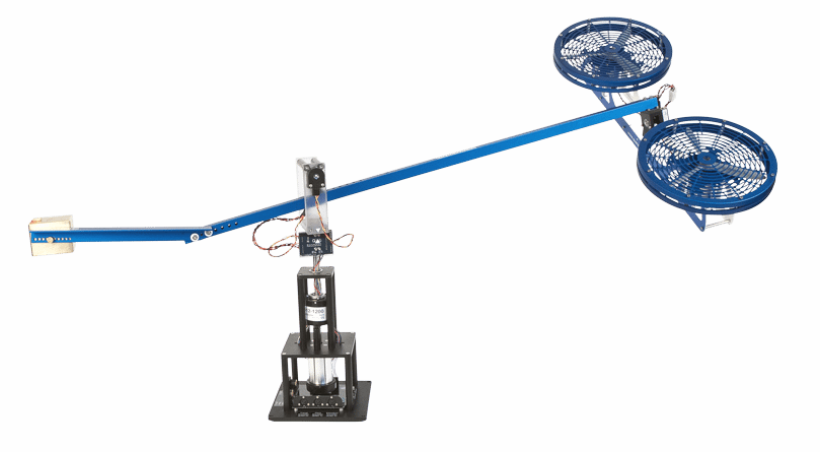
\includegraphics[scale=0.5]{fig/helicopter.png}
    \caption{Picture of Quanser's 3 DOF Helicopter}
    \label{fig:pic_heli}
\end{figure}

In addition, the helicopter comes with a Q8-USB 8 Channel USB Data Acquisition Board and the VoltPAQ-X2 2 Channel Linear Voltage Amplifier, also from Quanser. For Simulink use, it comes with the software package, QUARC.


Since this hardware is designed for testing and developing control laws for systems with similar dynamics, there is a lot of research done on this helicopter.

\cite{veeraboina_2018}: A simplified nonlinear model with LQR, LQR based PID, IO Feedback Linearizing and a Direct Adaptive Fuzzy Controller has been implemented on an Arduino Mega. 

\cite{arican_2018}: State-Dependent Riccati Equation based optimal control for a nonlinear system. Linear control method for nonlinear control is inconsistent. 

\cite{kocagil_2017}: Design methods for nonlinear systems. Review of State Dependent Riccati Equation based optimal control, Model Reference Adaptive Control and Sliding Mode Control. 

\cite{jafri_2017}: Design and apply a fuzzy logic controller. Fuzzy logic controller is a type of control based on fuzzy logic where logical variables take on continuous values between 0 and 1. This is an advantage when dealing with a complex, or "expensive" process model. Compared with a PID, it is concluded that the proposed controller performs better.

\cite{yang_2019}: Multiple helicopters, a fault-tolerant robust adaptive control algorithm is proposed that synchronizes multiple helicopters with actuator faults.

However, none of the existing control suggestion are very equipped for constraint handling. This is the advantage of \acrshort{mpc}. Some \acrshort{mpc}-implementations have been presented.

\cite{Zhai2010}: Nonlinear Model Predictive Control to control elevation and travel using successive linearization to approximate the internal model of the system, and performance is compared to linear \acrshort{mpc}.

Using \acrshort{nmpc} for the helicopter is not feasible given its fast dynamics. Helicopter control is 10 Hz, which is nearly impossible for microcontrollers to run at that speed using \acrlong{nmpc}.

\cite{Tondel2002}: Explicit piecewise linear state feedback solutions to constrained \acrshort{mpc} gives larger offline complexity. Paper studies two approaches to complexity reduction, input trajectory parametrization and search tree that allows PWL function to be implemented in real time. However, this deals with explicit \acrshort{mpc}. 

\cite{ju_2014}: \acrfull{empc} of the helicopter is presented in simulation and semi-physical simulation. Proves feasibility and performance of \acrshort{empc}-algorithm. 

\cite{cheng_2016}: \acrfull{empc} for attitude regulation and tracking, compared with a \acrshort{pid}-controller. 


\acrfull{empc} is a version of \acrshort{mpc} that reduces the online computational cost of the control by moving all those calculations offline. This entails providing an explicit optimal control law  by calculating all possible optimal input trajectories in the operating region of the system. 

This is not feasible because



The closest research to what is presented in this thesis:
\cite{Zhai2013}: An observer based \acrshort{mpc} with successive linearization, which uses the current state of the system to linearize a nonlinear process model about that point and use the linear model in the \acrshort{mpc}, online. This paper focuses on a performance comparison between the use of unscented Kalman filter and other filters, like linear filter and extended Kalman filter. The \acrshort{qp}-problem used in the \acrshort{mpc} is without a terminal constraint or cost.

The work presented in this thesis has a larger focus on the concept of \textit{stable} \acrlong{mpc} - the effects of adding a terminal cost and constraint.



\section{Embedded Optimization}


Embedded optimization is the concept of continuously solving an optimization problem where the data is update real-time from a system the evolves over time. Naturally, the exact evolution of the system can only be predicted to a certain degree, and the optimization should be dynamic, as in a function of time and the process. Embedded optimization is complex, mainly because of the close relationship between the solver, the hardware and the process \cite{embedded_optimization}.

In the late 1970s, \acrlong{mpc} was introduced as a combination of feedback control theory and numerical optimization \cite{mpc_early}, and quickly gained traction as a constraint handling control method, mostly used in the petrochemical and process industry. As the computer was introduced and popularized a few decades later, optimization methods on embedded hardware was introduced to address needs such as cost effectiveness and efficient energy use. Now the technology mostly used in a specific industry could be applied to areas such as robotics, aerospace and automotive. With this development challenges related to algorithms and their implementations, as well as the computing hardware arises. 

The concept of embedded \acrshort{mpc} arises from this development. Thirty years ago, this algorithm was run on computers at low frequencies, as slow as calculations once a minute \cite{qin_badgwell}. 

Over the last thirty years, a lot of \acrshort{mpc} implementations have been introduced, mostly solving the \acrshort{qp}-problem on a computer at a low frequency. However, more recently, solving these optimization problems on embedded hardware has been done for \acrfull{cpu}s, digital signal processors, programmable logic controllers and \acrfull{fpga}s \cite{embedded_optimization_control}.

The topic of embedded \acrshort{mpc} is an increasingly en popular one, as it is being proposed for smaller and smaller systems. \acrshort{mpc} has become an increasingly popular control method, given it can solve problems with physical constraints. The demand for this technology to work in embedded systems is only natural. An obstacle in this is the computational cost, and therefore time requirement. This is where, for example OSQP comes in, a \acrshort{qp}-solver perfectly suited for \acrshort{mpc} in embedded.

A few examples are using MPC for controlling a hovercraft, and a path following MPC for serial-link robot manipulators \cite{embedded_optimization_control}. 


The existing control solutions for embedded systems, \acrshort{pid}-controller, Kalman filter, \acrshort{lqr}, needs a lot of tuning to cope with constraints and nonlinearities. Introduction \acrshort{mpc} removes this problem. However, problems arise when considering the online computational cost of \acrlong{mpc}, therefore this concept warrants extra attention. 




%MPC THEORY





\chapter{Model Predictive Control Theory} \label{sec:MPC}



\section{QP-problem}

\acrfull{mpc}, also called \acrfull{rhc}, is a control strategy that implements an implicit control law by solving a constrained optimal control problem over a finite time horizon.

The basic idea behind \acrlong{mpc} is optimizing the systems state trajectory and resulting control input, given a finite-horizon cost function, for every time step and applying the first optimal control input to the system.

\acrshort{mpc} is one of the most attractive feedback strategies utilized, especially for constrained linear systems. 

The three main stages of the algorithm are
\begin{enumerate}
    \item Measuring the current state of the system
    \item Solving the given optimization problem
    \item Applying the first control input to the system, while the others are rejected
\end{enumerate}


Legg inn figure av MPC men bruk ekte tall fra systemet.
Altså ta 4 tidssteg av en tilstand pluss en optimal trajectory og optimal control input. 


If a nonlinear process model is used in the prediction, it is referred to as \acrfull{nmpc}, while a linear model is just \acrfull{mpc}. The advantages to using \acrlong{nmpc} are beyond the scope of this thesis, but in short the advantage is a more accurate process model leading to a more accurate prediction, but at the cost of computational cost and run-time. 

Even though a software framework for embedded \acrlong{nmpc} has been suggested, with sampling times in the millisecond range \cite{Englert2019}, this implementation relies on the software being compatible with QUARC. 

%Try to find the downside in this. You need at least one good reason for why you didn't do this. 

Linear \acrshort{mpc} is by far the most heavily used. It is less complex - in best case it can be a convex \acrshort{qp}-problem - and the feedback mechanism of \acrshort{mpc} can account for differences between the model and the actual system, which are certain to exist since a linear model will never be completely accurate in an actual process. It is used in this project, mainly because keeping the complexity of the optimization problem minimal is important as it will be running on an embedded system, with limited capacity. In addition the framework already written for this project in \cite{prosjekt_oppgave}, was made for a linear system model and the whole process becomes more complicated if \acrlong{nmpc} is used instead.

The basic formulation for the optimization problem solved in \acrshort{mpc} problem is,

\begin{equation}\label{eq:MPC_unstable}
    \begin{split}
        \mathbb{P}_n (x_0) \: = \: \min_{\bm x, \bm u} & \: \: \frac{1}{2} \sum_{j=0}^{{N-1}}(x_{n+1}^\top Q x_{n+1 } + u_{n}^\top R u_n) \: \: , \\
        \text{s.t. }    & x_{i+1} = Ax_i + Bu_i \: \forall \: i \in \mathbb{Z}_{[0:N-1]},\\
                        & x_i \in \mathbb{X} \: \forall \: i \in \mathbb{Z}_{[1:N]}  \: \: , \\
                        & u_i \in \mathbb{U} \: \forall \: i \in \mathbb{Z}_{[0:N-1]}    \: \: , \\
    \end{split}
\end{equation}
with 
\begin{equation}\label{eq:MPC_unstable_desc}
    \begin{split}
        x_i, \mathbb{X} &\in \mathbb{R}^n \: \: , \\
        u_i, \mathbb{U} &\in \mathbb{R}^m \: \: , \\
       Q, A &\in \mathbb{R}^{n\times n}, \: B \in \mathbb{R}^{n\times m} \: \: , \\
       R &\in \mathbb{R}^{m \times m} \: \: .
    \end{split}        
\end{equation}

The matrices $A$ and $B$ are the matrices for the state space model for the given system.

In addition, a few conditions to ensure nominal stability: the matrices $Q$ and $R$ must be real and symmetric, $Q$ must be positive semidefinite, and $R$ must be positive definite.

This problem formulation is used in a number of \acrshort{mpc} implementations, and can be shown to nominally stable %\cite{something}.

To keep this stable, one has to choose a rather large horizon $N$, which in turn increases the complexity of the problem. This trait is highly unwanted in embedded systems.


However, an extension to this problem can be made that has been proven ot [...]. 

Note that this problem optimizes the $N$-horizon constrained state and input trajectory based in the system dynamics and the current state of the system $x_0$. This takes place instead of the infinite-horizon optimization, because of constraint handling. However, adding the infinite-horizon trajectory to the cost function would be equivalent to optimizing on a infinite-trajectory where constraint-handling takes place in the first $N$-steps, and an LQR regulator is present after this, for $x_{N+1}, x_{N+2}, \hdots. $ 

This is just an abstract explanation of how the \acrshort{mpc} calculates the optimal trajectory and control input for each time-step. The control input applied to the actual system for each time step, considers the constraints.

Consider the potential infinite horizon cost function, but with the control law $u_k = Kx_{k}$,

\begin{equation}\label{eq:cost_inf_horizon}
    \begin{split}
        &\sum_{k=0}^{\infty} x_k^\top (Q + K^\top R K) x_k \: \: ,
    \end{split}
\end{equation}
and the state feedback matrix 
\begin{equation}\label{eq:feedback_matrix}
    K = -(R + B^\top P B)^{-1} B^\top P A \: \: ,
\end{equation}
where $P$ is the solution to the \acrfull{dare},
\begin{equation}\label{eq:DARE}
    A^\top P A - P + Q - A^\top PB(R + B^\top PB)^{-1}B^\top PA = 0 \: \: . \\
\end{equation}

Given equation \eqref{eq:feedback_matrix}, this can be written as,


\begin{equation}\label{eq:new_DARE}
    A_K^\top P A_K - P + Q + K^\top R K = 0\: \: ,
\end{equation}
with $A_K = A + B K $ being the new system matrix for 
\begin{equation}
    x^+ = A x + B u 
\end{equation}
with feedback control law $u = Kx$.

Inserting the revised equation \eqref{eq:new_DARE} into the infinite horizon cost function \eqref{eq:cost_inf_horizon}, but only considering the cost beyond the horizon $N$, yields
\begin{equation}
    \begin{split}
    &\sum_{k=N}^{\infty} x_k^\top (P - A_K^\top P A_K) x_k \\
    = &\sum_{k=N}^{\infty} x_k^\top P x_k - \sum_{k=0}^{\infty} x_{k+1}^\top P x_{k+1} \\
    = & x_N^\top P x_N \: \: .
    \end{split}
\end{equation}

This requires $(A, B)$ to be controllable, such that a solution to the \acrshort{dare} $P$ is positive definite and the eigenvalues of $(A-BK)$ is asymptotically stable.

Adding this term to the original \acrshort{mpc} problem adds a terminal cost such that the optimization considers a control law beyond the horizon, which results in a more stable control of the system.

This implies that the optimal state and control trajectory calculated at each time step, accounts for the fact that beyond the horizon the system will be controlled by an \acrshort{lqr}.

This result shows that it is possible to optimize on an infinite horizon, with a finite sum in the objective function. It is useful to note that the \textit{so called control} beyond the horizon will not ensure constraint satisfaction.

The idea is that the control input for the finite horizon handles the constraints so the \acrshort{lqr} controller is optimal for the rest of the horizon. \cite{optreg}
 
Rawlings and Mayne points out that, in light of this proof, it has been shown that there exists a set of initial states for which \acrshort{mpc} is actually optimal for the infinite horizon constrained optimal problem. 
 
These conditions are sufficient for \textit{nominal stability} of the control law. Meaning, in the absence of any disturbance, the above problem formulation is a stable version of \acrshort{mpc}. However, for most systems, disturbance is a reality and therefore one extra measure can be added to the problem to ensure stability. 

This is a terminal constraint on the last state, $x_N \in \mathbb{X}_f$ in an attempt to control the state trajectory past the horizon. 

"A detailed proof of the stability of nominal \acrshort{mpc} is outside the scope of this paper. However, the above derivations have hopefully given the reader an intuitive understanding of the contribution the terminal constraint set and terminal cost has to the stability of the \acrshort{mpc}."
    
Finally, consider the revised optimal control problem,

\begin{equation}\label{eq:MPC_stable}
    \begin{split}
        \mathbb{P}_s(x_0) \: = \: \min_{\bm x, \bm u}& \: \: \frac{1}{2} \sum_{j=0}^{{N-1}}(x_{j}^\top Q x_{j} + u_{j}^\top R u_j) + x_N^\top P x_N \: \: , \\
        \text{s.t. }    & x_{i+1} = Ax_i + Bu_i \: \forall \: i \in [0, N-1],\\
                        &  {x_{lb}}_i \leq x_i \leq  {x_{ub}}_i \: \forall \: i \in [1, N]  \: \: , \\
                        &  {u_{lb}}_i \leq u_i \leq  {u_{ub}}_i \: \forall \: i \in [0, N-1]    \: \: , \\
                        x_N \in \mathbb{X}_f \: \: ,
    \end{split}
\end{equation}
where the previous assumptions in \eqref{eq:MPC_unstable_desc} still applies, in addition to 
\begin{equation}\label{eq:MPC_stable_desc}
    \begin{split}
       P &\in \mathbb{R}^{n\times n}, \: B \in \mathbb{R}^{n\times m} \: \: , \\
    \end{split}        
\end{equation}

and $P$ has to be positive semi-definite. This is to ensure that a solution to the \acrlong{dare} exists.

This is a more stable version of the original \acrshort{mpc} description.
    
The revised cost function now includes the term $x_0^\top Q x_0$. This is merely because it makes the formulation easier, and this constant term will not effect the optimal solution.

For both formulations, the quadratic program is solved at every time step and the first control action $u_0$ is applied to the system.

\section{Reference tracking}

Another feature \acrshort{mpc} handles very well is reference tracking.
This is partially utilized in this project. If one aims for steering the helicopter from $\lambda = \lambda_{int}$ to $\lambda = 0$, the equilibrium point, then the $x^{\text{ref}}$ term disappears. And adding a constant term $\lambda_int$ to the $\lambda$ measurement in Simulink gives  the initial point that is wanted. 


\begin{equation}
    \sum (x_n - (x^{\text{ref}}_n)^\top Q (x_n - (x^{\text{ref}}_n) + u_n^\top R u_n \: \: .
\end{equation}

Another version of this is trajectory tracking, 

\section{Terminal constraint}\label{sec:terminal_constraint}

The selection of the terminal constraint is very important.

The idea is too select the largest feasible control invariant set possible.

This entails inserting the LQR controller $u = Kx$ into the system equation
\begin{equation}
    \begin{split}
        x^+ = A x + B u \: \: , \\
        C x + D u \leq e \: \: ,
    \end{split}
\end{equation}
to get
\begin{equation}
    \begin{split}
        x^+ = A_K x \: \: , \\
        C_K x \leq e \: \: .
    \end{split}        
\end{equation}

Then calculating the \textit{maximal positive invariant set} under these conditions. Requiring the last state of the optimal state trajectory to be in this set ensures stability past the horizon. 

Figure


One drawback of enforcing the terminal constraint, especially a constant terminal constraint calculated offline, is that starting out far from a equilibrium point with a short horizon, the problem becomes infeasible very easily. 

For example consider the helicopter starting out at $\lambda = 180 deg$ with N = 15. This initial point is infeasible, so \acrshort{mpc} control from this point is impossible.

A solution to this problem is moving terminal constraint, calculated online, which considers the current state of the system. This requires running on a system with enough computational power to calculate such things. This will be discussed in more detail later on. 


A concept known as \textit{recursive feasiblity}, described in Rawlings and Mayne \cite{Rawlings&Mayne}, implies that given the feasible region $X_n$ as a subset of $\mathbb{R}^n$, then for any initial state $x_0 \in X_n$, all subsequent states under the system model $x^+ = Ax + Bu$ also lie in $X_n$. However, as mentioned earlier, this only applies to the nominal system and for most systems with a disturbance, something can cause the state to become infeasible. This leads to the optimal control problem not having a solution, and the controller fails.

Choosing the terminal constraint to be the \textit{maximal invariant constraint admissible set} for $x^+ = (A + BK) x.$ This is the largest set W, such that $W \subset \{ x \in \mathbb{X} | Kx \in \mathbb{U} \}$ and $x \in W \rightarrow x_i = A_K^i x \in W$. Given this definition the terminal constraint set $\mathbb{X}_f$ is control invariant. If the initial state is in the terminal constraint set, the controller $u = Kx$ ensures the state trajectory stays in the set, under state and control constraints for all future time. 


\begin{equation}
    \mathbb{X}_f \subset \mathbb{X}, K \mathbb{X}_f \subset \mathbb{U} \: \: .
\end{equation}


The terminal constraints $\mathbb{X}_f$ is the set of states such that the evolution of the state trajectory stays in the set and satisfies the constraints, when $\bar{u} = K \bar{x}$. Chapter 2.6 in \cite{Rawlings&Mayne} addresses the necessity of the terminal constraint. 

"Addition of the terminal cost does not materially affect the optimal control problem"

The terminal constraint should have the property that for every $x \in \mathbb{X}_f$, there exists a feasible control input such that $x^+ = Ax + Bu \in \mathbb{X}_f$, $V_f(x^+) - V_f(x) \leq -l(x,u)$.


Terminal set: $\mathbb{X}_f = \{ x \in \mathbb{R}^n | V_f(x) \leq \alpha \}$ with $\alpha$ chosen by the designer such that $x \in \mathbb{X}, Kx \in \mathbb{U}.$

Another method is not enforcing the terminal constraint but just verified a-posteriori and increasing N if not satisfied. 

Useful lemma 2.40, page 145:
Given the optimal control trajectory for the terminally unconstrained optimal problem, the associated optimal state trajectory will not be in the terminal constraint set if the last state $x_N$ is not in the terminal constraint set. 


Even though the terminal constraint set is not always necessary, especially if there are no hard state constraints in the problem from before, it is deemed necessary for the control of the system discussed in this project. 



"If it is desired that the feasible sets are nested (ensuring recursive feasibility), it is necessary to include a terminal constraint. "



\section{Integral action in MPC}

\cite{Rawlings&Mayne} chapter 1.5.2 discusses this topic.
And chapter 5.
\cite{merging_opt_control} discusses this approach. 

Observe that the \acrshort{mpc}-controller behaves similar to a \acrshort{pd}-controller, in the sense that [...]. As a parallel, these controllers don't have integral action, so removing residual errors can be a challenge. There are many ways for embedding integral action into \acrlong{mpc}. 

\cite{Rawlings&Mayne} (ch.1.5.2) discusses the concept of constructing an \acrshort{mpc}-controller to achieve zero offset. They state that this method is "similar to what one achieves when using the integral mode in \acrshort{pid}-control of an unconstrained system". \cite{Rawlings&Mayne} (page 49).

Most methods aimed at zero offset use the same approach. Firstly, model the disturbance. Secondly, use the actual measurements and model to estimate the disturbance. Lastly, find the inputs that minimize the effect of the disturbance. 

The approach discussed in \cite{merging_opt_control} will be presented here. 


The helicopter simulation used in the practical aspect of this thesis and described in detail in section \ref{sec:helicopter} has an unfortunate flaw in its design. The two propellers spin in the same direction, which causes a constant torque around the travel axis and therefore a constant drift in the travel. 

This can be noted in the initial simulations of the helicopter presented in chapter \ref{ch:results}. Obviously, this constant deviation is problematic if this system and this controller is to be of any practical use. 

A simple solution to this constant deviation is modeling the constant disturbance to the travel as a state to the state space model. Then, by adding implementing a state estimator to estimate its value, the optimization, and therefore the current control action, will account for the disturbance. This method is described in \cite{merging_opt_control}, as well as below. 

Adding a \textit{Luenberger observer}.

The error dynamics, defined by 
\begin{equation}
    e^+ = (A - LC) e \: \: ,
\end{equation}
converges to zero if one selects the estimator gain $L$ such that $(A-LC)$ has all the eigenvalues inside the unit circle.


Augmenting the state space model yields,
\begin{equation}
    \begin{split}
        \m{ x^+ \\  d^+} &= \m{A & A_d \\ 0 & 1} \m{ x \\  d} + \m{B \\ 0} u \: \:, \\
        y &= \m{C & C_d} \m{x \\ d} \: \: .
        \end{split}
\end{equation}

For simplicity sake, in this section $x^+ = Ax + Bu, \: y = Cx$ will be used to describe the augmented system dynamics.

The state observer,
\begin{equation}
    \begin{split}
        \hat x &= A \hat x + B u + L^\top ( y - \hat y) \: \: , \\
        \hat y &= C \hat x \: \: ,
    \end{split}
\end{equation}
gives the error dynamics $e = x - \hat x$,
\begin{equation}
    \begin{split}
        e^+ = (A - LC) e \: \: .
    \end{split}
\end{equation}

This observer, \textit{the prediction observer}, predicts the state in the next time step based solely on past measurements. It does not depend on the most current measurement, which causes the observer to perform worse.

Check this out
 This needs to be checked out. In simulink it looks like this isn't the case
An alternative observer, \textit{the current observer}, is suggested,
\begin{equation}
    \begin{split}
        \bar x^+ = \hat A \hat x + \hat B u \: \: , \\
        \hat x = \bar x + L(x - \bar x) \: \: ,
    \end{split}
\end{equation}
which yields the error dynamics,
\begin{equation}
    e^+ = (A - LA) e \: \: .
\end{equation}

The optimal solution is using a kalman filter, otherwise referred to as \textit{a linear quadratic estimator (LQE)}. The kalman filter assumes the system model is 
\begin{equation}
    \begin{split}
        \tilde x^+ = \hat A \tilde x + \hat Bu + \hat Ew \: \: , \\
        y = \hat C \tilde x + v \: \: ,
    \end{split}
\end{equation}

where $w$ is a disturbance on the system and $v$ is measurement noise. These are assumed to be white Gaussian noise with zero mean and zero correlation and a given covariance. With this knowledge, the kalman filter calculates an observer gain matrix $K_f$ that minimizes the variance of the estimation error $e$. However, this observer requires that the covariance of the process and measurement noise be known, which isn't always the case. In addition, this observer is better suited for systems with a lot of dynamic disturbance. It is already established that the disturbance present in the helicopter system is constant and easy to model.



\section{Slack variables}
A common issue when implementing \acrshort{mpc} as a controller, is the possibility that the system enters into a state which makes the optimization problem infeasible. This is common when there is a disturbance in the system, such that the system dynamics varies slightly from the prediction of the \acrshort{mpc} controller.

In this case, a slack variable $\epsilon_p$ is added to the constraint on the pitch and to the cost function as $s \epsilon_p^2$. This was found to be necessary mainly because this constraints is not a hard constraint. It is implemented primarily to attempt to keep the system as close to the equilibrium point as possible, so the linearized model stays relatively accurate.

There is also a question of how many slack variables and whether to have different ones for the upper and lower constraint, and different variables for each time step. 



Having the same variable over a horizon saves a lot in regards to complexity but it comes at a cost. When the slack variable is the same for the whole horizon, any constraint violation at any point will allow for constraint violation over the whole horizon without any extra cost. Therefore, this will lead to a much less stable control of the system. 

If the lower and upper constraints are weighted separately, consider having a different slack variable for each one. 


\section{Stability of MPC}


This section will talk about the stability of MPC. Stability criteria, and some proofs.

\section{Robustness of MPC}
A nominal stability analysis is out of the scope of this thesis. However, analysing the potential robustness of the method is seen as useful.

Demonstrating robustness for an uncertain system is important, especially when the disturbance is not known. 

[Talk about robustness here]



A way to ensure robustness is using tube-based model predictive control, a version of model predictive control that ensures that the state trajectory will always be contained in a tube with the nominal state trajectory, given the assumptions on the disturbance hold, by tightening the state and control constraints. 

The resulting control problem when attempting to control the given system using this model and the given implementation is too complex so this idea was abandoned quite early in the process.

However, there are ways to ensure robustness, even when the system disturbance is unknown. 

Robust control of this system has been attempted in [], however no literature on robust \acrshort{mpc} has been publically available.





\section{Pre-stabilization}


Given the optimal control problem for \acrshort{mpc} described in equation \eqref{eq:MPC_stable}, there is a slight adjustment to the algorithm that can reduce the complexity of the problem. 

Define a new optimal control trajectory $\bm c = \m{c_0 & c_1 & \hdots & c_{N-1}}^\top,$ and a new control law, 

\begin{equation}\label{eq:mpc_feedback_control_law}
    u_k = c_k + K x_k \text{, for  } k \in \mathbb{Z}_{[0:N-1]} \: \: .
\end{equation}

This in turn leads to an augmented control problem, where this variation in control input is taken into consideration.

For this, the problem formulation presented in equation \eqref{eq:MPC_stable}, is used as the starting point. Replacing the control input $u_k$ with $c_k$ using equation \eqref{eq:mpc_feedback_control_law}, results in,


\begin{equation}\label{eq:MPC_stable}
    \begin{split}
        \min_{\bm x, \bm c}& \: \: \frac{1}{2} \sum_{n=0}^{{N-1}}(x_{n}^\top \tilde Q x_{n} + c_n^\top R c_n + 2 c_n^\top R^\top K x_n ) + x_N^\top P x_N \: \: , \\
        \text{s.t. }        & x_0 \text{ given} \: \: , \\
                            & x_{i+1} = A_k x_i + Bc_i \: \forall \: i \in [0, N-1],\\
                            &  {x_{lb}}_i \leq x_i \leq  {x_{ub}}_i \: \forall \: i \in [1, N]  \: \: , \\
                            &  {u_{lb}}_i \leq c_i + Kx_i \leq  {u_{ub}}_i \: \forall \: i \in [0, N-1]    \: \: , \\
                           & x_N \in \mathbb{X}_f \: \: ,
    \end{split}
\end{equation}
where
\begin{equation}
  \tilde Q = (Q + K^\top R K) \:, A_K = A + BK \: \: .
\end{equation}

This new formulation gives an identical performance as the other \acrshort{mpc}. However, it also gives a guaranteed asymptotically stable system matrix $A_K$, because $K$ is chosen by the designer. This method, known as \textit{pre-stabilization}, reduces the complexity of the calculations made when removing the equality constraints, shown in section \ref{sec:remove_eq_constr}. When $A_K$ is asymptotically stable, calculating $A_K^i$ does not increase as $i$ increases. The system described in this project has an asymptotically stable system matrix, so this method is not necessary.  


\section{Removing equality constraints}\label{sec:remove_eq_constr}
 
The standard \acrshort{mpc} problem, described in previous works, will be reformulated to fit the \acrshort{qp}-problem used in the implementation of OSQP. 
It is recognized that another possibility is just letting $lb$ = $ub$. However, there are more benefits to removing equality constraints altogether, as will become evident.

A reformulation will be used that optimizes over the same function with only inequality constraints. The benefits of this will become clear (it involves a lower triangular matrix). 

The problem solves in OSQP is presented below, 

 \begin{equation}
 \begin{split}
\min \: &\frac{1}{2} z^\top P z + q^\top z \: \: , \\
\text{subject to } l &\leq Az \leq u \: \: .
\end{split}
 \end{equation}


Starting with the discrete system equation, 
\begin{equation}
    x^+ = A x + B u \: \: ,
\end{equation}
one can note the following development.
 
 \begin{equation}
     \begin{split}
         x_1 &= A x_0 + B u_0 \\
         x_2 &= Ax_1 + Bu_1 \\
             &= A(Ax_0 + Bu_0) + Bu_1 \\
             &= A^2 x_0 + AB u_0 + Bu_1\\
        x_3 &= Ax_2 + Bu_2 \\
            &= A(A^2 x_0 + ABu_0 + Bu_1) + Bu_2 \\
            &= A^3 x_0 + A^2Bu_0 + ABu_1 + Bu_2 \\
             & \: \vdots \\
        x_k &= A^{k-1}B u_{0} + A^{k-2} Bu_{1} + \hdots + B u_2 + A^k x_0
     \end{split}
 \end{equation}
 \begin{equation}
 \begin{split}
     \m{x_1 \\ x_2 \\ \vdots \\ x_N } &= \m{B & 0 & \hdots & 0 & 0 \\ AB & B & \hdots & 0 & 0 \\  & & \vdots & \\ A^{N-1} B & A^{N-2} B & \hdots & AB & B} \m{u_0 \\ u_1 \\ \vdots \\ u_{N-1}} + \m{A \\ A^2 \\ \vdots \\ A^N} x_0  \\
\end{split}     
\end{equation}
One can write this as 
\begin{equation}\label{eq:xSuSx}
    \bm x = S_u \bm u + S_x x_0 
\end{equation}
with
\begin{equation}
    \bm x = \m{x_1 \\ x_2 \\ \vdots \\ x_N} \text{ and } \bm u = \m{u_0 \\ u_1 \\ \vdots \\ u_{N- 1}}.
\end{equation}
Inserting equation \eqref{eq:xSuSx} into the objective function gives the following development,
\begin{equation}
\begin{split}
    \phi &= ( \sum_{n=0}^{N-1} x_{n+1}^\top Q_{n+1}
    x_{n+1} + u_n R_n u_n ) + x_N^\top P x_N \\
    &= \bm x^\top \bar{Q} \bm x + \bm u^\top \bar{R} \bm u \\
    &= (S_u \bm u + S_x x_0)^\top \bar{Q} (S_u \bm u + S_x x_0) + \bm u^\top \bar{R} \bm u \\
    &= \bm u^\top S_u^\top \bar{Q} S_u \bm u + x_0^\top S_x^\top \bar{Q} S_x x_0 + \bm u^\top S_u^\top \bar{Q} S_x x_0 + x_0^\top S_x^\top \bar{Q} S_u \bm u + \bm u^\top \bar{R} \bm u \\
    &= \bm u^\top ( S_u^\top \bar{Q} S_u + \bar{R} ) \bm u + 2 x_0^\top S_x^\top \bar{Q} S_u \bm u + x_0^\top S_x^\top \bar Q S_x x_0 \: \: ,
    \end{split}
\end{equation}
with 
\begin{equation}
    \bar Q = \m{Q_1 & & & \\
               & Q_2 & & \\
               & & \ddots \\
               & & & Q_{N-1} \\
               & & & & P}, \: \: \bar R = \m{R_0 & & \\
               & R_1 & \\
               & & \ddots \\
               & & & R_{N-1}} \: \: . \\
\end{equation}

Noting that a constant sum of the objective function is redundant to the solution of the \acrshort{qp}-problem, the objective function for OSQP becomes
\begin{equation}
    \phi = \frac{1}{2} z^\top P z + q^\top z \: \: ,
\end{equation}
with
\begin{equation}
    P = 2 S_u^\top \bar{Q} S_u + \bar{R}, \: \:  q = 2 S_u^\top \bar{Q} S_x x_0 , \: \: z = \bm u \: \: .
\end{equation}

The problem can now be formulated as,

\begin{equation}\label{eq:prob_no_eq_constr}
    \begin{split}
    \min_{z}  & \: \:  \phi \: \: , \\
    \text{subject to } & \: \: S_u z + S_x x_0 \in \mathbb{X} \: \: , \\
                       & \: \: z \in \mathbb{U} \: \: , \\ 
                       & \: \: {S_u}^{\text{row}_N} z + {S_x}^{\text{row}_N} x_0 \in \mathbb{X}_f  \: \: .     
    \end{split}
\end{equation}

 

                                                        


%MODELL

\chapter{Developing a process model}


\section{Helicopter Model}\label{sec:helicopter}

A figure of the helicopter simulation can be seen in figure \ref{fig:heli_1}. An actual photograph is shown on the front page of this thesis.

\begin{figure}
    \centering
    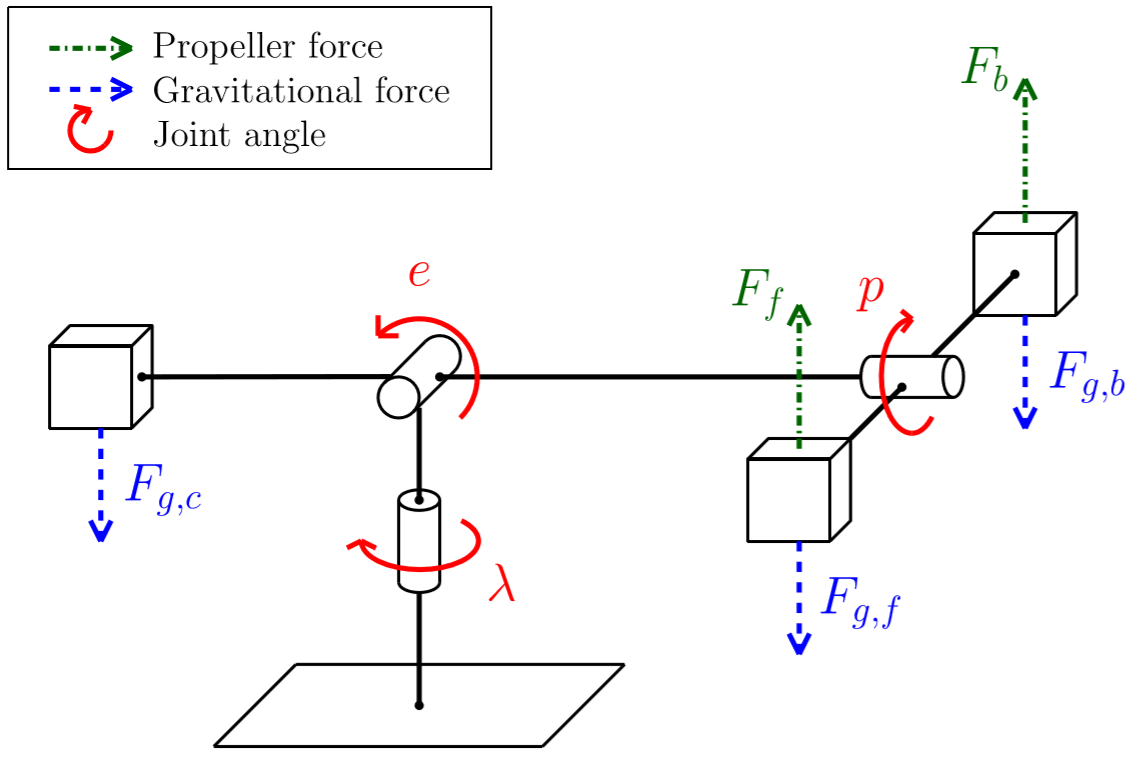
\includegraphics[scale=0.5]{fig/heli_fig_1.png}
    \caption{Figure of helicopter forces}
    \label{fig:heli_1}
\end{figure}

Starting with Newton's second law of rotation for the three system states travel $\lambda$, pitch $p$ and elevation $e$, which states that the net external torque equals the product of the moment of inertia and the angular acceleration,
\begin{equation}
    \begin{split}
        J_{\lambda} \ddot{\lambda} &= \sum{\tau_{\lambda}} \\
        J_p \ddot{p} &= \sum{\tau_p} \\
        J_e \ddot{e} &= \sum{\tau_e} \: \: .
    \end{split}
\end{equation}

Note that all friction, both aerodynamic drag and friction in the joints is neglected.

It is assumed that the the forces generated by the propellers is proportional to the voltages applied,
\begin{equation}
    \begin{split}
        F_f = K_f V_f \: \: ,\\
        F_b = K_b V_b \: \: ,
        \end{split}
\end{equation}
where $K_f$and $K_b$ are the proportionality constants.

Starting with the travel $\lambda$, the net external torque will  
\begin{equation}
    J_{\lambda} \ddot{\lambda} = (V_b - V_f) l_h \cos{e} \sin{p} \: \: .
\end{equation}

For the pitch $p$, the contributions are the propellers force, such that 
\begin{equation}
    J_{p} \ddot{p} = F_f l_p  - F_b l_p  \: \: .
\end{equation}

For elevation $e$, the contributions are the propellers affected by the angle of the pitch as well as the weight of both arms, such that 
\begin{equation}
    J_{e} \ddot{e} = (F_f + F_b)l_h \cos{p} -2 m_p g l_h  \cos{e} + m_c g l_c \cos{e}  \: \: .
\end{equation}
Denoting the voltage difference $V_f - V_b$ as $V_d$, and the voltage sum $V_f + V_b$ as $V_s$ in addition to defining the following constants,
\begin{equation}
    \begin{split}
        L_1 &= K_f l_p \: \: , \\ 
        L_2 &= g(m_c l_c  - 2 m_p l_h) \: \: , \\
        L_3 &= K_f l_h \: \: ,\\ 
    \end{split}
\end{equation}
the following system equations are presented,
\begin{equation}\label{eq:nonlin_heli}
    \begin{split}
        J_{\lambda} \ddot{\lambda} &= -L_3 V_s \cos{e} \sin{p} \: \: ,\\ 
        J_p \ddot{p} &= L_1 V_d \: \: ,\\ 
        J_e \ddot{e} &= L_2 \cos{e} + L_3 V_s \cos{p} \: \: .\\ 
    \end{split}
\end{equation}

Since \acrshort{mpc} solves a \acrshort{qp}-problem at every time step, the system equations in \eqref{eq:nonlin_heli} will be  linearized around the helicopters equilibrium point. This calculation is described in appendix \ref{ch:linear_heli_model}.

The resulting first-order discrete linear time system is 

\begin{equation}
    \begin{split}
        x^+ &= Ax + Bu \: , \: \: \\
        A &= \m{1 & h & 0 & 0 & 0 & 0 \\
                0 & 1 & -hK_2 & 0 & 0 & 0 \\
                0 & 0 & 1 & h & 0 & 0 \\
                0 & 0 & -hK_1 K_{pp} & 1-hK_1 K_{pd} & 0 & 0 \\
                0 & 0 & 0 & 0 & 1 & h \\
                0 & 0 & 0 & 0 & -hK_3 K_{ep} & 1-hK_3 K_{ed}}, \\
        B &= \m{0 & 0 \\ 0 & 0 \\ 0 & 0 \\
                h K_1 K_{pp} & 0 \\ 0 & 0 \\ 0 & h K_3 K_{ep}} \: \: ,
    \end{split}
\end{equation}
with $x = \m{\lambda & \dot{\lambda} & p & \dot p & e & \dot e }^\top$, $u = \m{p_c & e_c}^\top$.



\section{Modelling constant disturbance} \label{sec:estimator}

As described above, the offset described is a constant drift in the travel, so
\begin{equation}
    A_d = \m{1 \\ 0 \\ 0 \\ 0 \\ 0 \\ 0 }^\top \: \: . 
\end{equation}

The implementation of the state estimator and the modelling of the constant disturbance seems simple enough. 


The results of how the estimator performs is presented in section \ref{sec:results}, Results. 

\subsection{Choosing poles for estimator gain $L$}

The strategy for choosing poles in discrete time is choosing them in a continual time space and then transforming them to poles in the discrete time space using the equation,
\begin{equation}
    z = e^{h \cdot p} \: \: ,
\end{equation}
where p is the pole in the continual time space, h is the sampling frequency, and z is the new pole in the discrete time space. 

Legg til figure

When selecting poles for state observers, it is important that the slowest eigenvalue of $A-LC$ is "faster", i.e. more negative than all the eigenvalues of $A - BK$. The placement of the poles in the left half plane also determine the step response of the error dynamics of the observer, however this is not as important, as long as the step response is stable and approaches zero faster than the state dynamics $A - BK$. 

The poles chosen for calculating the estimator gain where
\begin{equation}
    \begin{split}
        p = \m{0.3 \\ 0.4 \\ 0.5 \pm 0.15 i \\ 0.52 \pm 0.05 i \\ 0.6} \: \: .
    \end{split}
\end{equation}

Using the MATLAB function \verb|place(A,B,eig||, which calculates the matrix $K$ such that $A - BK$ has the eigenvalues given in $eig$. For the estimator gain, the code used was:
\begin{lstlisting}
L = place(system.A', system.C', p];
\end{lstlisting}

This because to use the place function for $A - BK$, where $A$ and $B$ are inputs, the symmetric system matrix for the observer $A_L = A - LC$ = $A_L^\top = A^\top - C^\top L^\top$.

The \textit{principle of separation of estimation and control} states that choice of observer gain $L$ and the choice of state feedback $K$ are independent of one another. This can be shown easily by looking at the complete system model
\begin{equation}
    \m{x^+ \\ e^+} = \m{A-BK & BK \\ 0 & A-LC} \m{x \\ e} \: \: .
\end{equation}
Since this is an upper triangular matrix, the eigenvalues of the system are just the eigenvalues of $A - BK$ and $A - LC$
%\cite{https://math.stackexchange.com/questions/21454/prove-that-the-eigenvalues-of-a-block-matrix-are-the-combined-eigenvalues-of-its}.
The stability of these two states are not dependent on each other
%\cite{https://en.wikipedia.org/wiki/Separation_principle}.


\section{Selection of constraints}

The only hard constraints on the states are there to reflect the limitations of the actual system. The pitch angel is limited, because this axis on the helicopter does not go all the way around. The elevation is also limited, mostly due to the table. 

One of the hard constraints on the travel, $\lambda$, is there to ensure feasibility. As mentioned in section \ref{sec:terminal_constraint}, starting too far away from the equilibrium point results in infeasibility, because of the terminal constraint. Therefore a hard constraint on $\lambda$ is only there to avoid infeasibility during run-time. 


The soft constraint $-30 deg - \epsilon_p \leq p \leq 30 deg + \epsilon_p$ is added, where $\epsilon_p \geq 0$ is also an optimization variable. This is so the linearized model will stay accurate, because $\sin p \approx p$ for small values of p.

PLOT



%HARDWARE IMPLEMENTATION

\chapter{Hardware and Software Implementation}\label{sec:methodology}


\section{OSQP}

OSQP (Operator Splitting Quadratic Program) is a \acrshort{qp}-solver developed at the University of Oxford. The main algorithm \cite{osqp}, developed in 2018.

"The algorithm is \acrfull{admm}, using a novel operator splitting technique that
requires the solution of a quasi-definite linear system with the same coefficient matrix
in each iteration." 

Alternating direction method of multipliers solves convex optimization problems using a divide-and-conquer method by breaking the problem up into smaller pieces. It takes the iterative method from the augmented Lagrange method and forces decomposability, giving it a smoother convergence but also a faster runtime.


A shortcoming of this algorithm that is worth mentioning, the convergence time is dependent on the user's choice of step-size parameters. However, the selection of optimal ADMM parameters is still open for discussion\cite{admm_param}. 

Since this algorithm in particular can solve optimization problems to a relative degree of certainty while still using few iterations, therefore being computationally inexpensive, it has been deemed a practical use for embedded processors. 


In addition to the extensive open-source MATLAB interface, it also offers a software package in MATLAB, among others, that can generate C code tailored to a specific quadratic program \cite{osqp-codegen}. This functionality is used in this project to generate C code deigned specifically for the \acrshort{mpc} \acrshort{qp}-problem, and can then be updated at every time step, using the C-interface.

The fact that this solver has both a MATLAB and C code interface, and a code generation software package, made it perfect to use in this project, where both running a simulation in MATLAB, and using  C code in the Simulink model was important. 


\begin{figure}
    \centering
    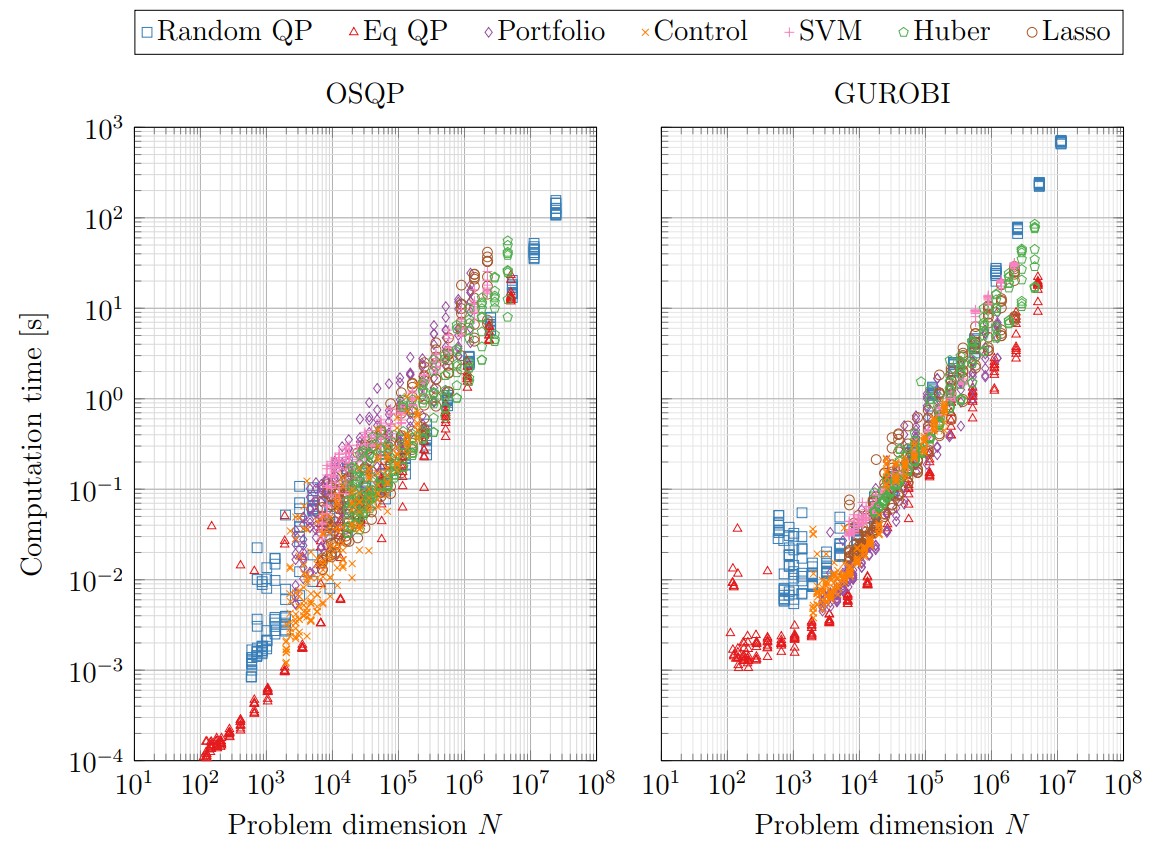
\includegraphics[scale=0.4]{fig/benchmark_osqp.png}
    \caption{Computation time vs problem dimension for OSQP and GUROBI for the 7 benchmark problem classes \cite{osqp}, page 20}
    \label{fig:osqp_benchmark}
\end{figure}

Figure \ref{fig:osqp_benchmark}, taken from \cite{osqp}, demonstrates the computation time of the OSQP-solver and the GUROBI-solver for 7 benchmark problems, and clearly demonstrates OSQP has a clear advantage in most of the problem. Specifically, the optimal control problem which is similar to the online problem for \acrshort{mpc}, performs slightly better with OSQP. 


\section{Simulink Model}

The basis for the Simulink model is the model already written for the helicopter, written by Andreas Flåten for the course TTK4135. 

See appendix \ref{sec:simulink_model_pic} for pictures of the Simulink model.

The helicopter interface \ref{fig:simulink_heli_interface}, pitch and elevation controller \ref{fig:simulink_pitch_contr}, \ref{fig:simulink_elev_contr} and voltage conversion block \ref{fig:simulink_Vd_Vs_block} were taken from the Simulink model used for the Helicopter Lab in TTK4135. 

The additions, are the \acrshort{mpc}-block \ref{fig:MPC} and the estimator \ref{fig:simulink_estimator} which were developed specifically for this project. 

The estimator-block is a Luenberger observer, implemented to estimate the disturbance affecting the system.

was implemented and can be seen here \ref{figure 3}. And the S-Function Builder which contains the \acrshort{mpc} implementation, in C code. 


The S-Function Builder generates the code for the main function of the implementation, and uses the problem description in the file 'workspace.h'. 

It was quickly realized that although the original quadratic program was generated in C code, because of the use of \acrshort{mpc}, this problem changes for every iteration. Both the linear cost $q$ and the upper bound $ub$ depend on the current state of the system $x_0$.

To recalculate the linear cost and the upper bound online, the matrices $bin, cin$ and $f$ had to be defined in C code. Therefore, a simple MATLAB script is used to define the datastructures \verb|c_float bindata[]| as strings in MATLAB and add these to the bottom of the file 'workspace.h', so they can be used by the \acrshort{mpc}-block.

For the version with inequality constraints, $ub$ and $lb$ are the constraints that must be updated. 


\subsection{S-Functions}
MATLAB 2015b is the version of MATLAB used in this project, and the corresponding Simulink version.

S-Functions are one of the functionalities of Simulink that is compatible with QUARC and code generation, so this was used to incorporate OSQP into the Simulink model. 


An S-Function is a Simulink block described in a computer language, in this case,  C. It is documented that S-Functions written in C/C++ are compatible with QUARC, with given known limitations \cite{quarc-s-function}. 

In this project the \textit{S-Function Builder} was used. This Simulink-block automatically generate the C-code necessary for an S-Function, with existing C-code supplied to it. The block generates a wrapper, which is in turn invokes when the model is run. The builder also generates a \verb|.tlc|-file, that describes how to inline the C-code during code generation. 



\section{Hardware In The Loop}

The hardware in the lab is supplied, ready made, by Quanser. 

%https://www.quanser.com/products/3-dof-helicopter/#overview 

The helicopter is a 3 DOF helicopter and is produced and sold by Quanser. along with all the other hardware in the lab. It is a bench top model of a Tandem rotor helicopter %\cite{https://www.quanser.com/products/3-dof-helicopter/#overview}. 
It has two propellers in parallel driven by DC-motors. The helicopter is equipped with three high-resolution encoders to measure the pitch angle between the propellers, the elevation angle, and the travel angle. 

\cite{user_manual_q8_board}
The helicopter is mounted in a slip ring which allows for 360 degree movement in the travel angle.

The hardware controlling the helicopter consists of the Q8-USB 8 Channel USB Data Acquisition Board and the VoltPAQ-X2 2 Channel Linear Voltage Amplifier from Quanser.

The board is an I/O card made for prototyping and Hardware-In-The-Loop development, and receives the signals from the helicopter, which is equipped with sensors. The amplifier receives the system inputs from the written control software supplied by the user and applies voltage to the propellers.


\begin{figure}
    \centering
    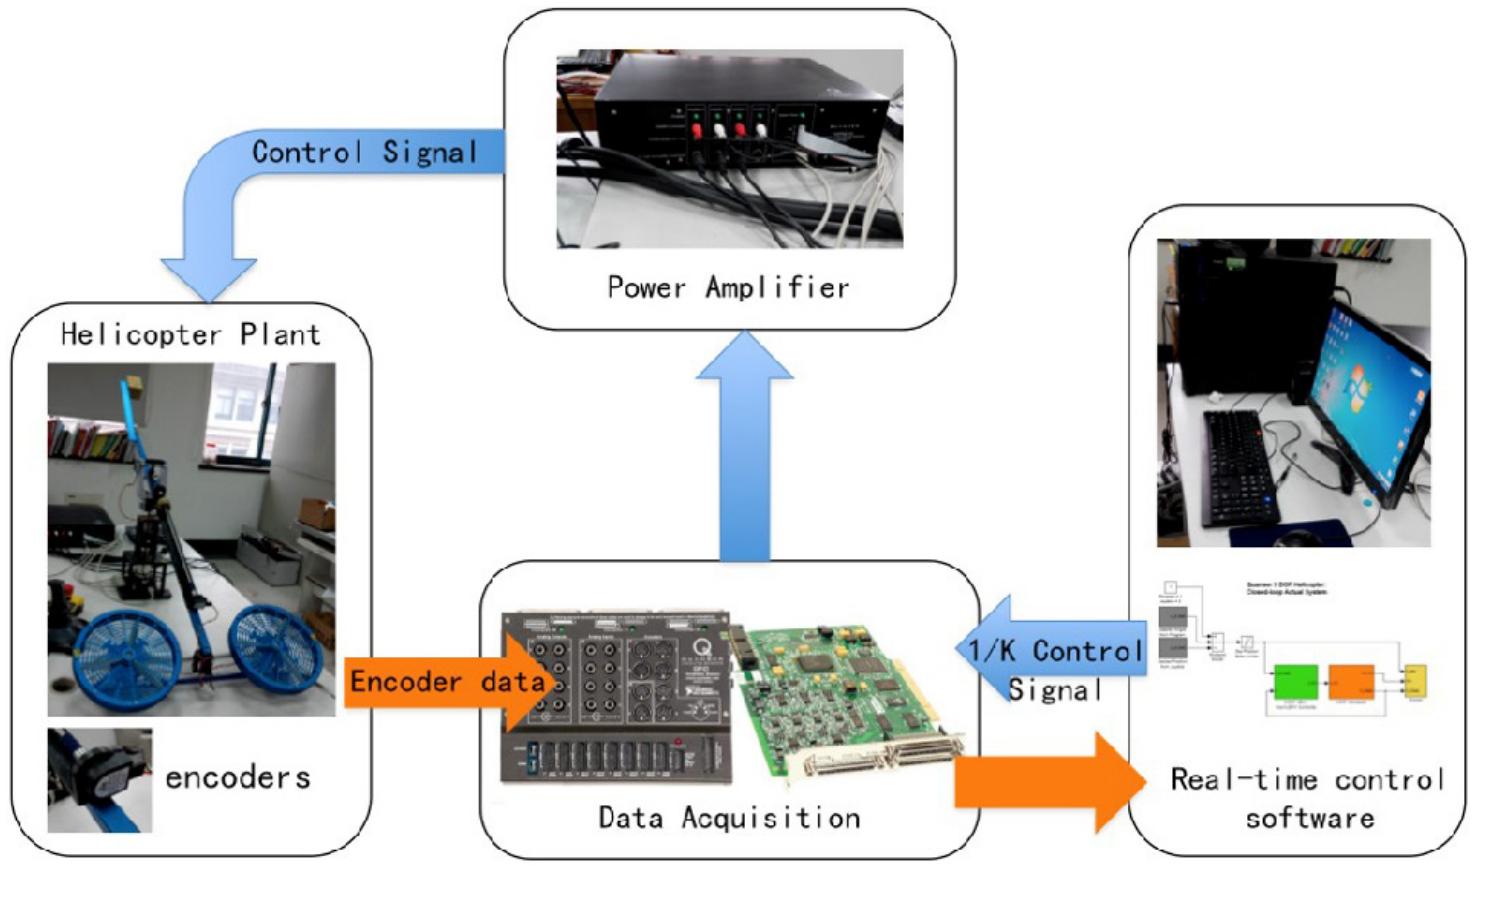
\includegraphics[scale=0.3]{fig/HIL_figure.png}
    \caption{Figure of HIL architecture, stand in}
    \label{fig:hil_architecture}
\end{figure}

Figure \ref{fig:hil_architecture} shows a diagram of the Hardware In The Loop setup. 

\textbf{QUARC}

In addition to the hardware described above, Quanser's 3 DOF helicopter package also comes with QUARC Real-Time Control Software for MATLAB and Simulink. 

"It extends the code generation capabilities of Real-Time Workshop (now called Simulink Coder). It adds a new set of targets the can change the source code generated by Real-Time Workshop to suit the particular platform. QUARC then compiles and links this code with relevant libraries and downloads the code on to the target, which is the Q8 Board. QUARC also has External Mode Communications that allows for connection to the target in Simulink and seeing the signals in real time. 

QUARC has Hardware-In-The-Loop functionality. It has numerous HIL blocks for Simulink, that allows one to use the signals from the board in the Simulink model.

The Simulink blocks written by QUARC that are used in the Simulink model are 
\begin{itemize}
    \item HIL Initialize 
    \item HIL Read Encoder Timebase 
    \item HIL Write Analog
\end{itemize}

There are first for initialization, writing voltage data to the I/O card and reading sensor information from the helicopter so it can be utilized in the Simulink model.

The reading encored block allows for an online visual of all the system signals. Which is why this software is designed for prototyping and testing.


\section{Multi-threading - different sampling times}

\begin{figure}
\centering
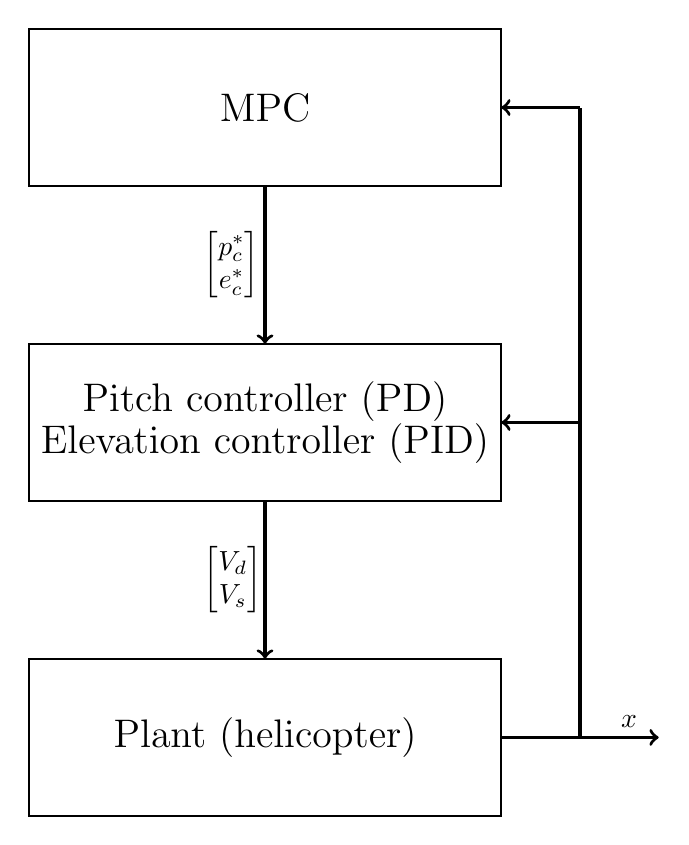
\begin{tikzpicture}[every text node part/.style={align=center}]

\draw[black, very thick, ->] (3,1) -- (5,1); %x
\draw[black, very thick, ->] (0,4) -- (0,2); %V_d V_s
\draw[black, very thick, ->] (0,8) -- (0,6); %*u
\draw[black, very thick] (4,1) -- (4,9); %bended arrow 1
\draw[black, very thick, ->] (4,5) -- (3,5); %bended arrow 1
\draw[black, very thick, ->] (4,9) -- (3,9); %bended arrow 2

\draw[black, thick] (-3,0) rectangle (3,2) node[pos=.5] {\Large {Plant (helicopter)}};
\draw[black, thick] (-3,4) rectangle (3,6) node[pos=.5] {\Large{Pitch controller (PD)} \\ \Large{Elevation controller (PID)}};
\draw[black, thick] (-3,8) rectangle (3,10) node[pos=.5] {\Large{MPC}};

\node[anchor=east, text width=4.4] (note1) at (4.8,1.2) {$x$};
\node[anchor=east, text width=4.4] (note2) at (-0.5, 3) {$\m{V_d \\ V_s}$};
\node[anchor=east, text width=4.4] (note2) at (-0.5, 7) {$\m{p_c^* \\ e_c^*}$};
\end{tikzpicture}
\caption{Diagram of system control architecture} \label{fig:system_arch}
\end{figure}

Figure \ref{fig:system_arch} shows a diagram of the system architecture. The highest level of control, the \acrshort{mpc}, should have a lower frequency than the rest of the system, so the lower level controllers have time to reach the given reference value before a new one is calculated.

In a Simulink simulation, a model cannot have modules that are running at different sampling intervals, as Simulink does not support this feature. QUARC, however, does. 

QUARC supports multi-threading, so blocks running on different sampling intervals are simply split into multiple threads, grouped together by sampling rate.  \cite{http://quanser-update.azurewebsites.net/quarc/documentation/quarc_multithreading.html}

When dealing with numerous levels of control, the higher levels of control should run at a lower frequency then the lower levels. 

The \acrshort{mpc} inputs reference values for the lower levels of control, so giving the system a little time to reach the reference before a new one is given, is desirable. 

In this simulation, the lower levels of control have a sampling time of 0.02 seconds, which is 50 Hz. The \acrshort{mpc} is run with 10 Hz, 5 Hz and 2 Hz.

An issue that is encountered when changing the frequency of the \acrshort{mpc} block, is the fact that the model used for the calculation is relatively inaccurate. As mentioned, it is linearized about the equilibrium point, so the inaccuracy increases further away from this point. 

When the frequency of the \acrshort{mpc}-calculations are lower, the system has longer time to develop this inaccuracy before the new state is fed back to the \acrshort{mpc}. This causes an oscillation in both the system and the optimal first state at each timestep. A suggested solution to this problem is using nonlinear model predictive control. This would lead to more accurate control without needing to run the higher level of control at such a high frequency. This is discussed further in chapter \ref{ch:discussion}, after the results from this phenomenon are presented.  



\section{Generating the \acrshort{mpc} problem}

The constraints for $x \in \mathbb{R}^n$ and $u \in \mathbb{R}^m$ are implemented as 
\begin{equation}
    \begin{split}
        Cx + Du \leq e \: \: , \\
        G x_n \leq h \: \: , \\
        C, G \in \mathbb{R}^{a\times n}, \: \: D \in \mathbb{R}^{a \times m} \: \: ,
    \end{split}
\end{equation}
with $a$ being the number of constraints.

With the constraint of the form $\bar C \bm x + \bar D \bm \leq \bar e$, this becomes
\begin{equation}
    \begin{split}
        &\m{C & & & \\
            & C & &   \\
             & & \ddots  & \\
             &  & & C \\
             & & & G} \bm x + \m{D & & & \\
            & D & &  \\
             & & \ddots &  \\
             &  & & D \\
             0 & 0 & \hdots & 0} \bm u \leq \m{e \\ e \\ \vdots\\ e \\ h}\: \: .
    \end{split}
\end{equation}

Inserting $x = S_u u + S_x x_0$, results in 
\begin{equation}
    \begin{split}
        &\bar C(S_u u + S_x x_0) + \bar D u \leq e \: \: , \\
        &\bar C S_u u + \bar C S_x x_0 + \bar D u \leq e \: \: , \\
        &(\bar C S_u + \bar D) u \leq \bar e - \bar C S_x x_0 \: \: .
    \end{split}
\end{equation}

Since $x_0$ is a variable, in the sense that it changes for every timestep, therefore for every call of the online calculations, the constraints are split up as follows,

\begin{equation}
    A_{in} x \leq b_{in} + c_{in} \cdot x_0 \: \: ,
\end{equation}
where
\begin{equation}
    A_{in} = \bar C S_u + \bar D\: \: , b_{in} = \bar e \: \: , c_{in} = -\bar C S_x \: \: .
\end{equation}



The MATLAB implementation of this can be found in listing \ref{lst:gen_mpc}. 


\subection{Calculating the terminal constraint}

The theory for terminal constraints was presented in \ref{sec:terminal_constraint}. There are many ways of approximating this, depending on the complexity of the system. In this implementation, the maximal control invariant set was used for the terminal constraint. 


\begin{equation}
    \m{1 & 0 & 0 & 0 & 0 & 0 & 0 & 0 \\
       -1 & 0 & 0 & 0 & 0 & 0 & 0 & 0 \\
       0 & 0 & 1 & 0 & 0 & 0 & 0 & -1 \\
       0 & 0 & -1 & 0 & 0 & 0 & 0 & -1 \\
       0 & 0 & 0 & 0 & 0 & 1 & 0 & 0\\
       0 & 0 & 0 & 0 & 0 & -1 & 0 & 0 \\
       0 & 0 & 0 & 0 & 0 & 0 & 0 & 1 \\
       1.3 & 3.9 & -2 & -0.6 & 0 & 0 & 0 & 0 \\
       -1.3 & -3.9 & 2 & 0.6 & 0 & 0 & 0 & 0 \\
       1 & 0.08 & 0 & 0 & 0 & 0 & 1 & 0 \\
       -1 & -0.08 & 0 & 0 & 0 & 0 & -1 & 0 \\
       0 & 0 & 1 & 0.08 & 0 & 0 & 0 & 0 \\
       0 & 0 & -1 & -0.08 & 0 & 0 & 0 & 0 \\
       0 & 0 & 0 & 0 & -0.03 & 0.9 & 0 & 0 \\
       0 & 0 & 0 & 0 & 0.03 & -0.9 & 0 & 0 \\
       1.1 & 3.3 & -1.6 & -0.5 & 0 & 0 & 1.3 & 0 \\
       -1.1 & -3.3 & 1.6 & 0.5 & 0 & 0 & -1.3 & 0} \m{\lambda \\ \dot \lambda \\ p \\ \dot p \\ e \\ \dot e \\ d \\ \epsilon_p} \leq \m{3.7 \\ 3.7 \\ 0.5 \\ 0.5 \\ 10000 \\ 10000 \\ 0 \\ 0.4 \\ 0.4 \\ 3.7 \\ 3.7 \\ 0.5 \\ 0.5 \\ 1000 \\ 1000 \\ 0.4 \\ 0.4}
\end{equation}

\section{MATLAB Simulation}

%SOFTWARE IMPLEMENTATION
%\chapter{Software Implementation}

%RESULTS
\chapter{Results}\label{ch:results}

The results from both a simulation in MATLAB and a simulation on the actual helicopter are presented here.


\section{Helicopter simulation in MATLAB}

The plots from the simulation in MATLAB are presented here. 


Below are plots of the helicopter equations simulated in MATLAB.

The system is simulated with a generated disturbance sequence, which is described in section \ref{sec:methodology}. The values are $10 \: deg \leq w \leq 12\:  deg.$


The finite horizon for the \acrshort{mpc} is $N = 15$.

First, the simulation without a terminal cost or terminal constraint.

\begin{figure}[h!]
    \centering
    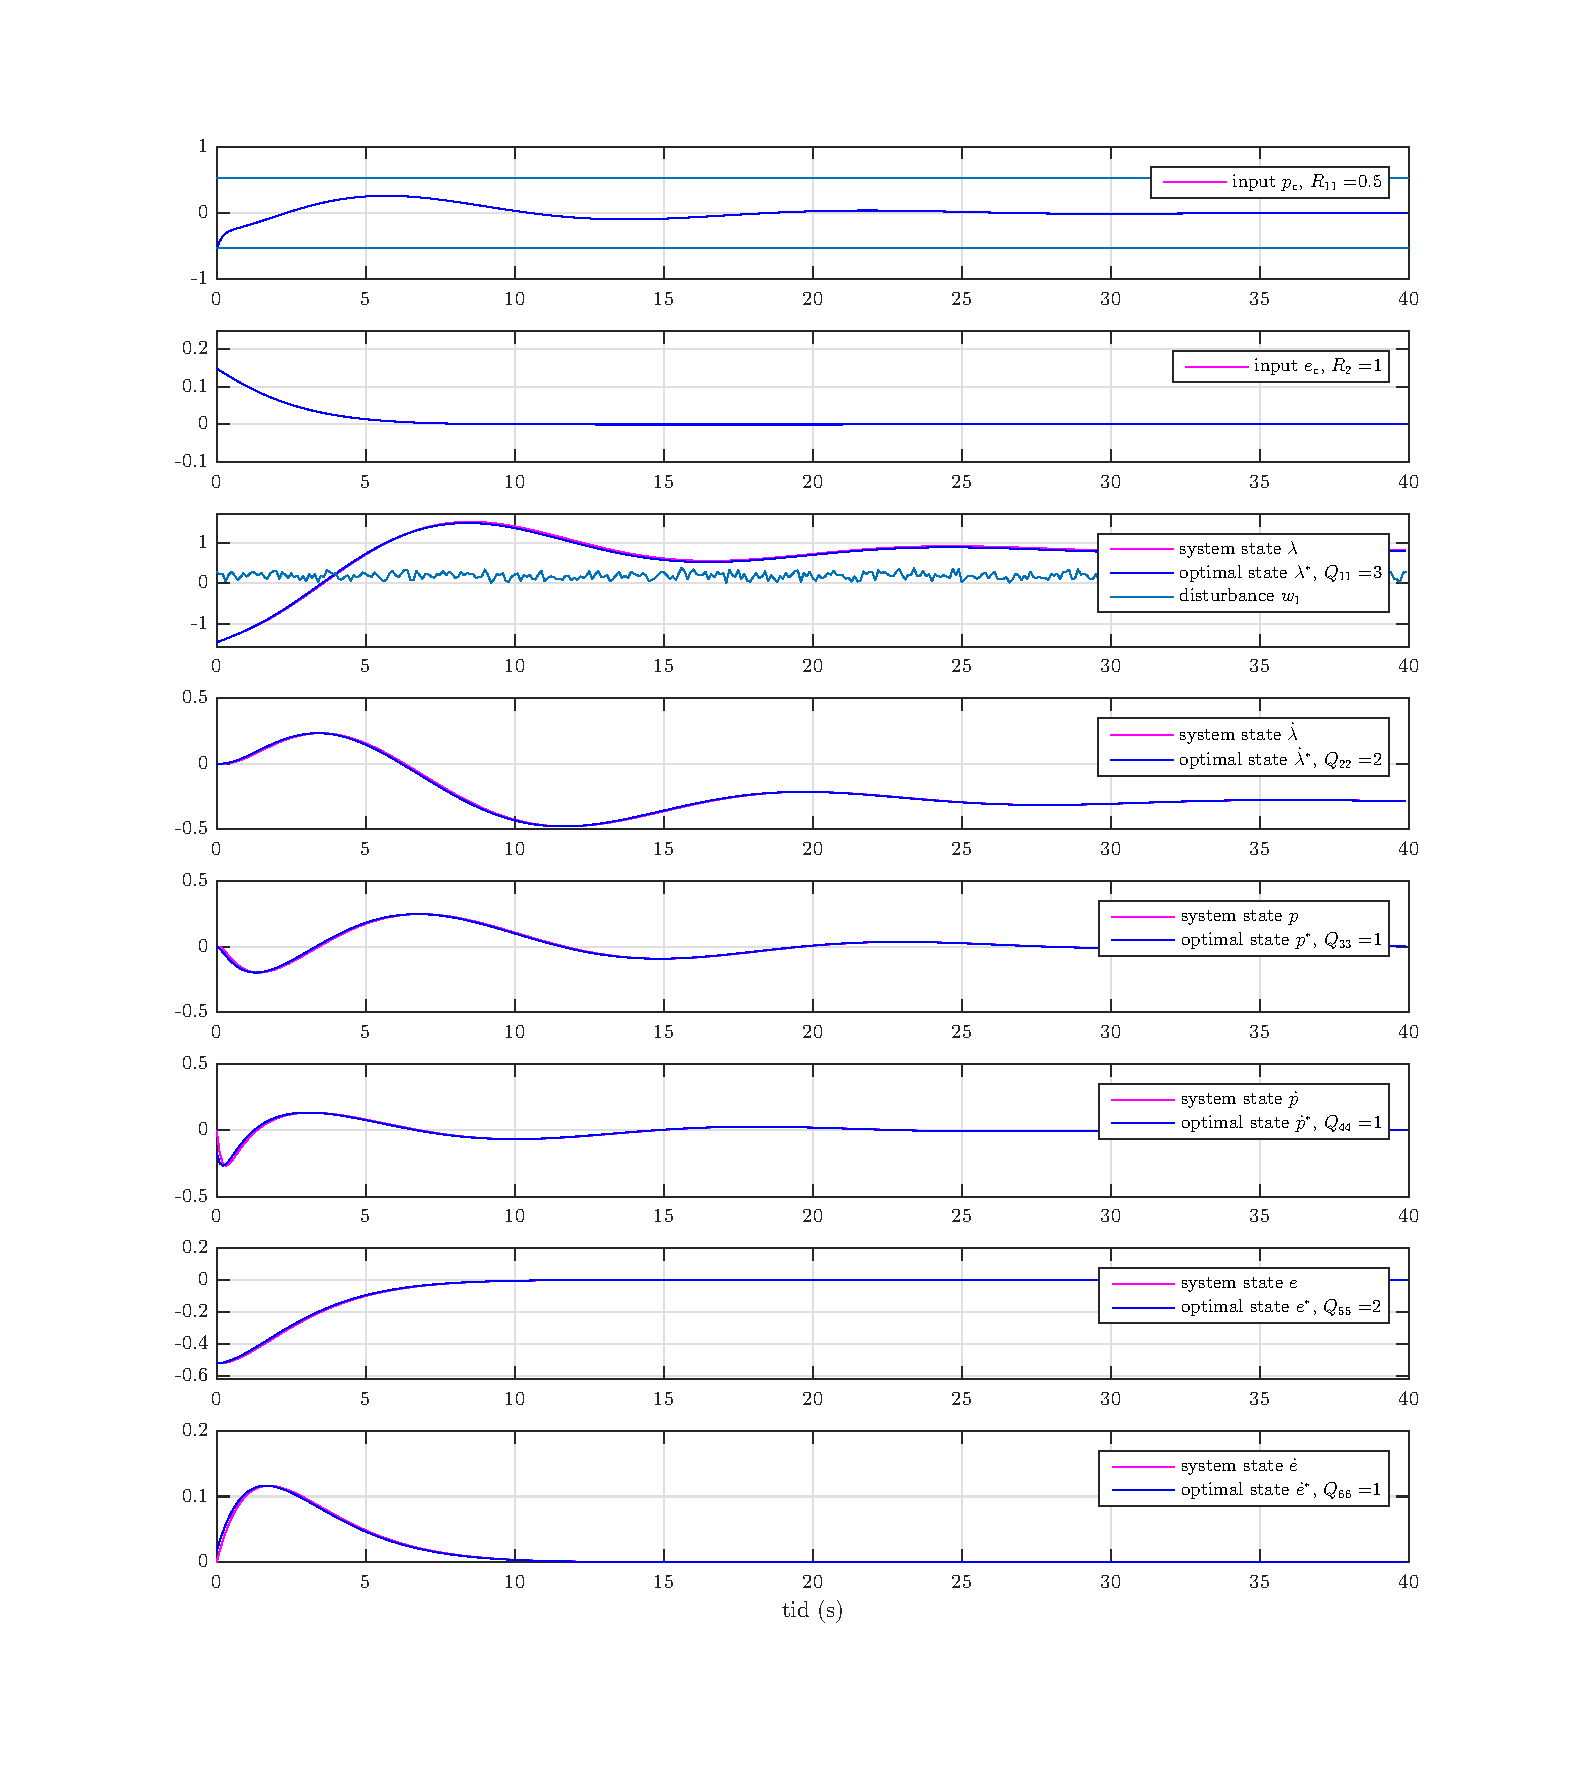
\includegraphics[scale=0.4]{fig/heli_sim_no_est_not_stable_extended_horizon.eps}
    \caption{Simulation in MATLAB with nominal \acrshort{mpc}}
    \label{fig:my_label}
\end{figure}

The travel $\lambda$, after 30 seconds, varies between $[0.7778, 0.8282]$. 

Further, the estimator described in section \ref{sec:estimator} is implemented. The goal is to model the disturbance applied, to try to remove the constant deviation in $\lambda$. 

\begin{figure}[h!]
    \centering
    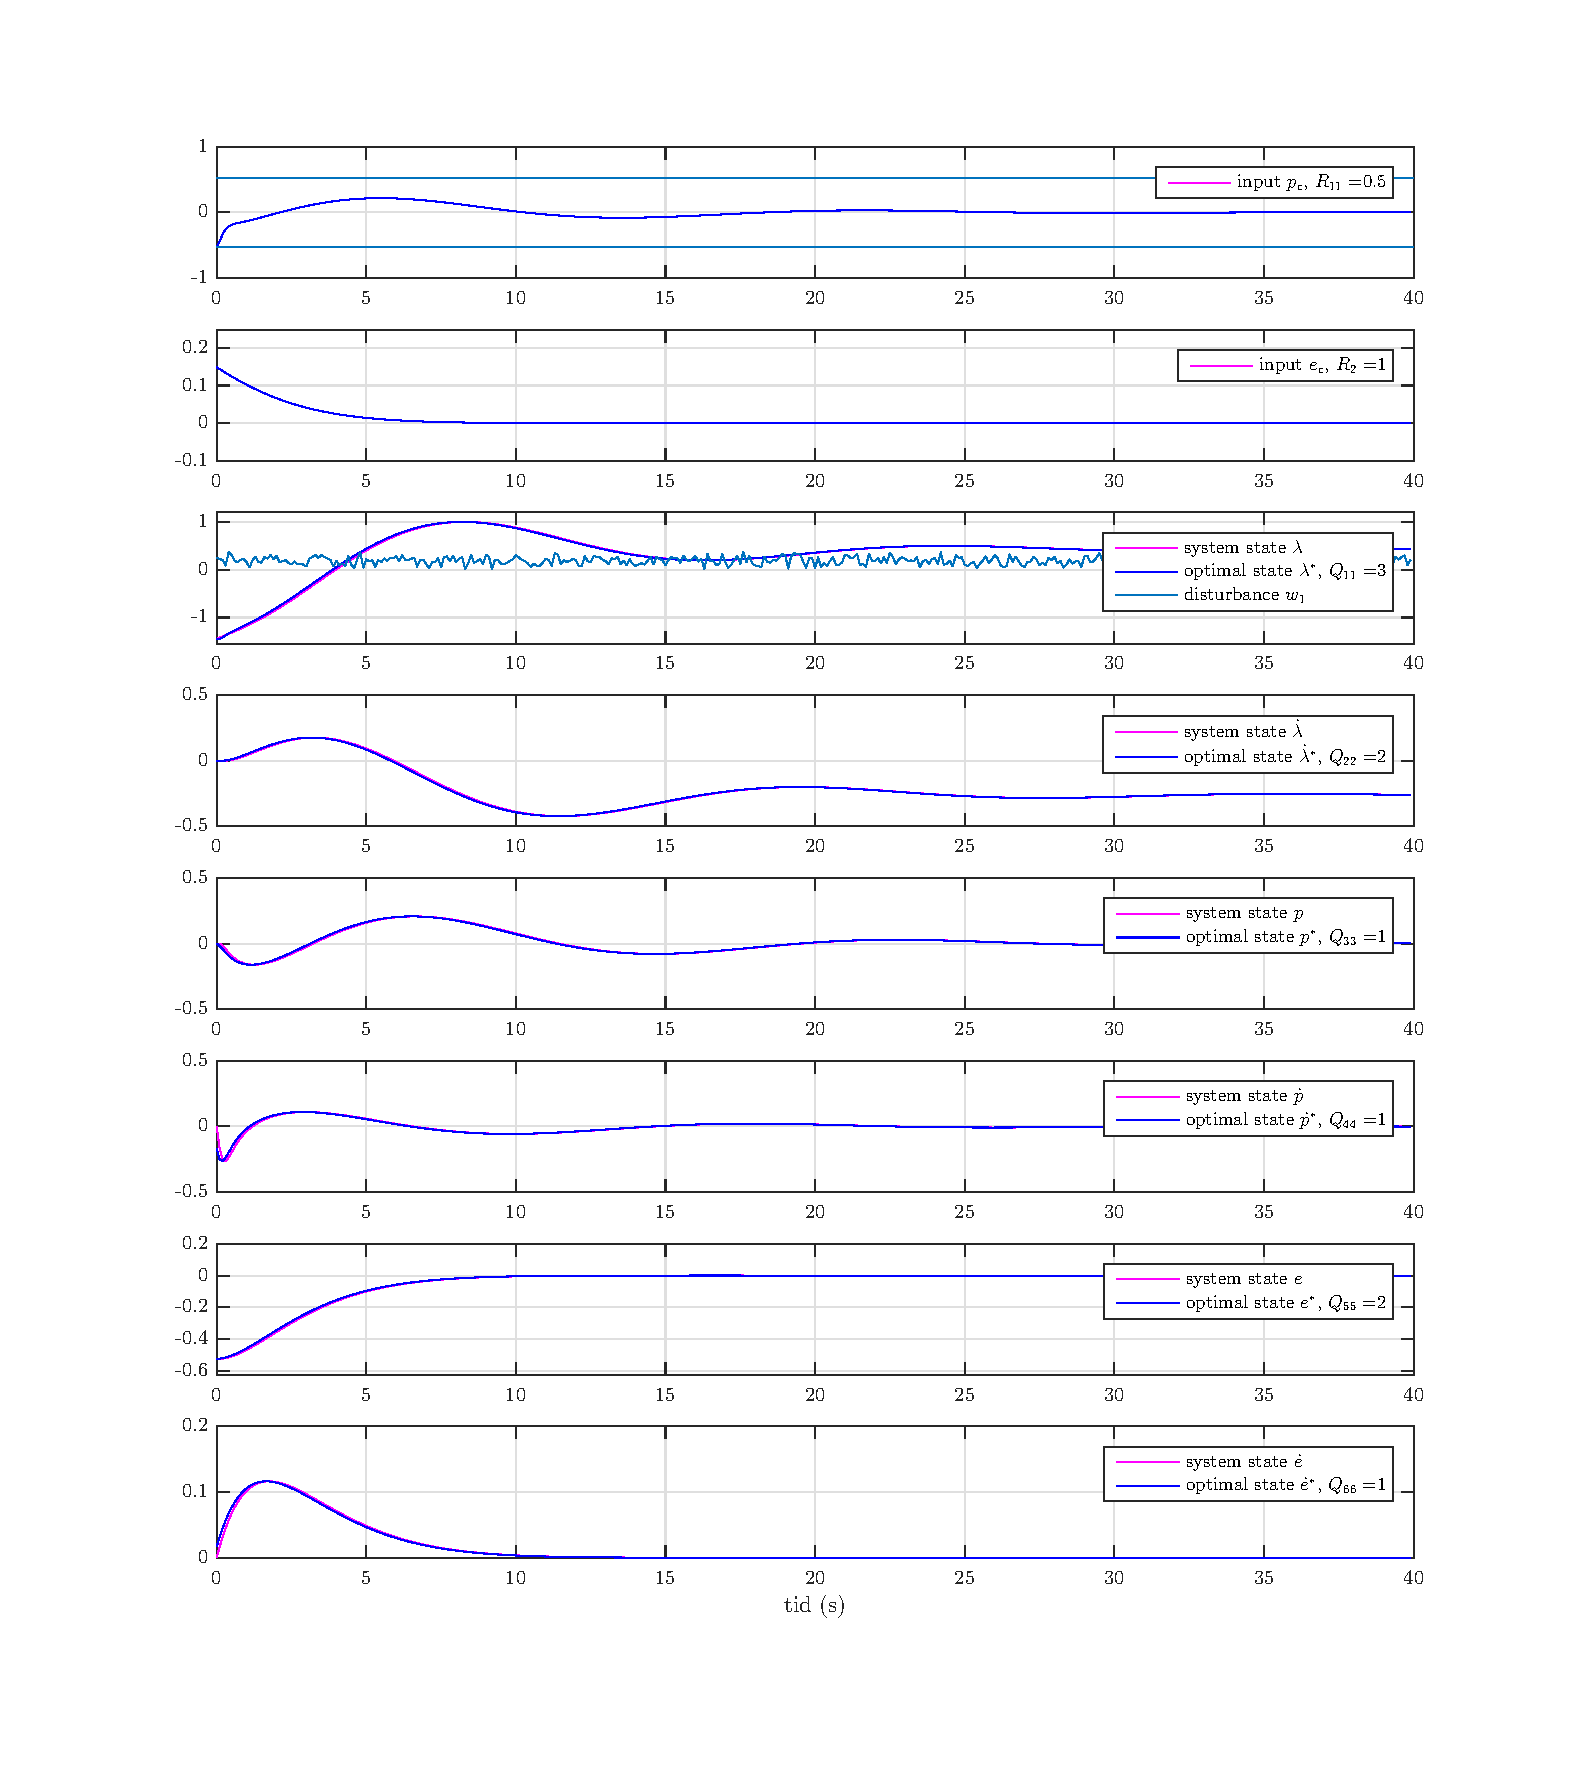
\includegraphics[scale=0.4]{fig/heli_sim_est_not_stable_extended_horizon.eps}
    \caption{Simulation in MATLAB with nominal \acrshort{mpc} and estimator}
    \label{fig:my_label}
\end{figure}

The travel $\lambda$, after 30 seconds, varies between $[0.3752, 0.4175]$. 

A plot of the error dynamics of the estimator is also shown, in addition to the estimator disturbance.

\begin{figure}[h!]
    \centering
    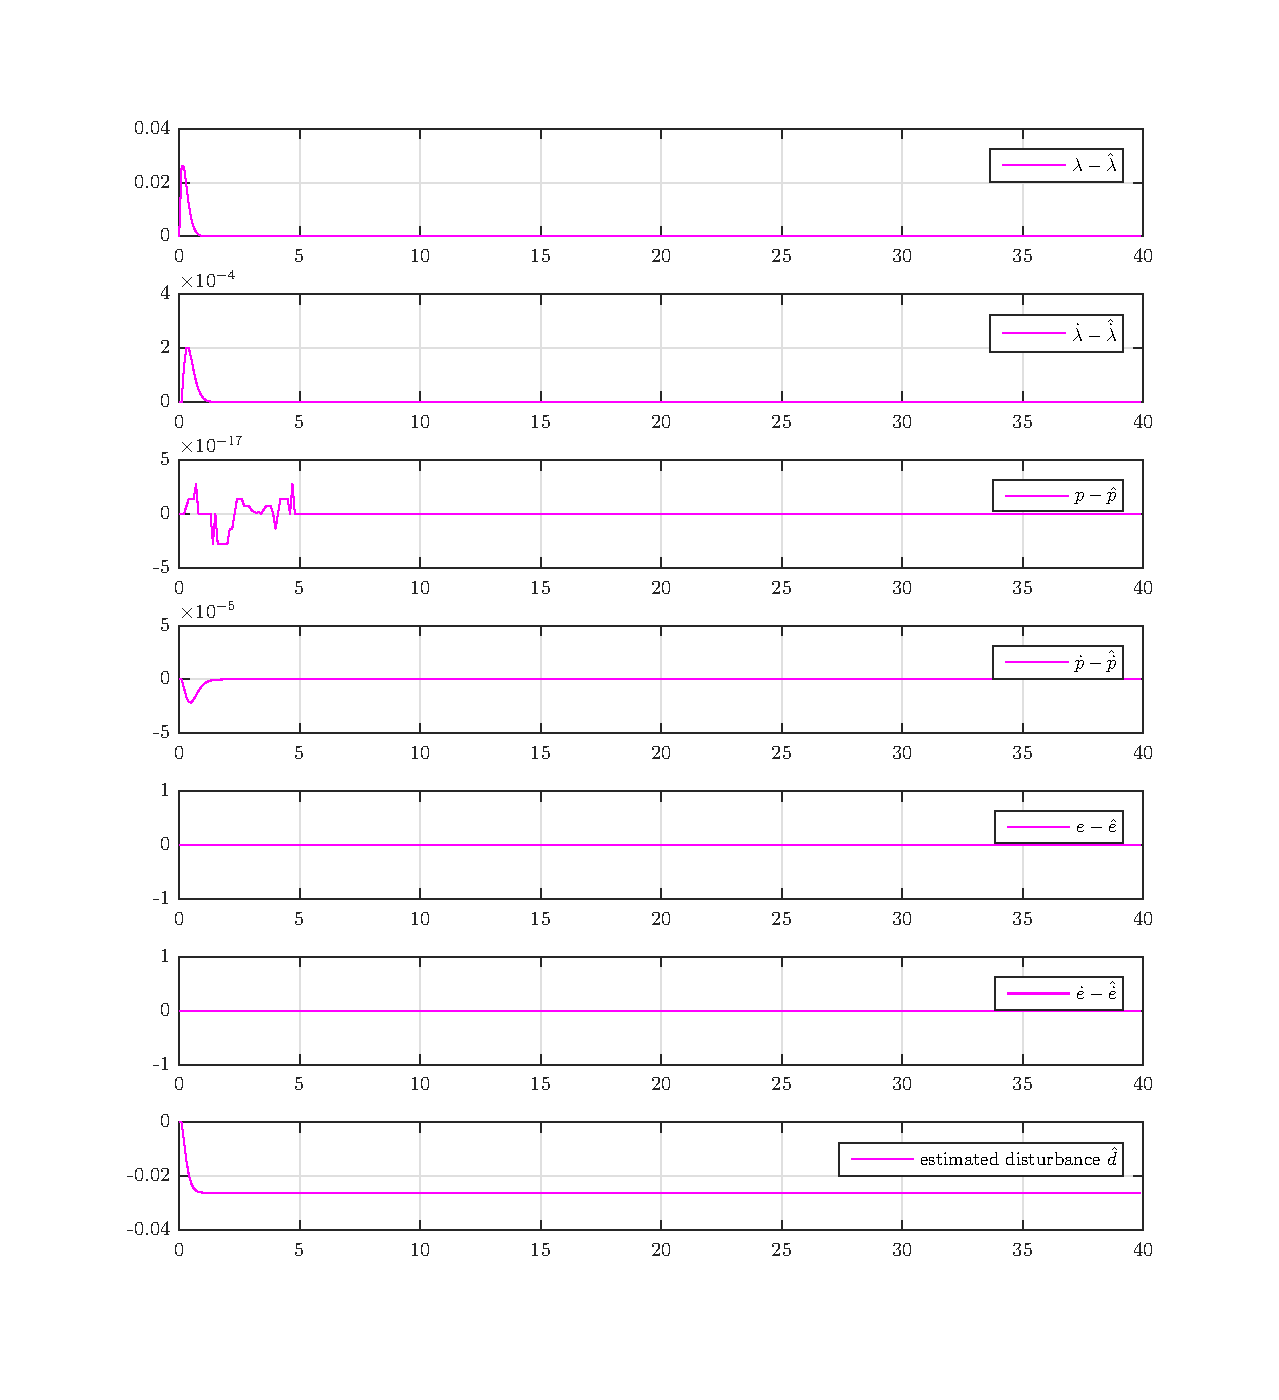
\includegraphics[scale=0.5]{fig/heli_sim_est_not_stable_extended_horizon_error_plot.eps}
    \caption{Error dynamics of estimator with nominal \acrshort{mpc}}
    \label{fig:my_label}
\end{figure}

Now, a terminal constraint and a terminal cost is added to the \acrshort{mpc}. These are described in section \ref{sec:MPC}. 

Firstly, the simulation without an estimator.

The simulation time is halved, because the helicopter tends towards the equilibrium point much faster. 

\begin{figure}[h!]
    \centering
    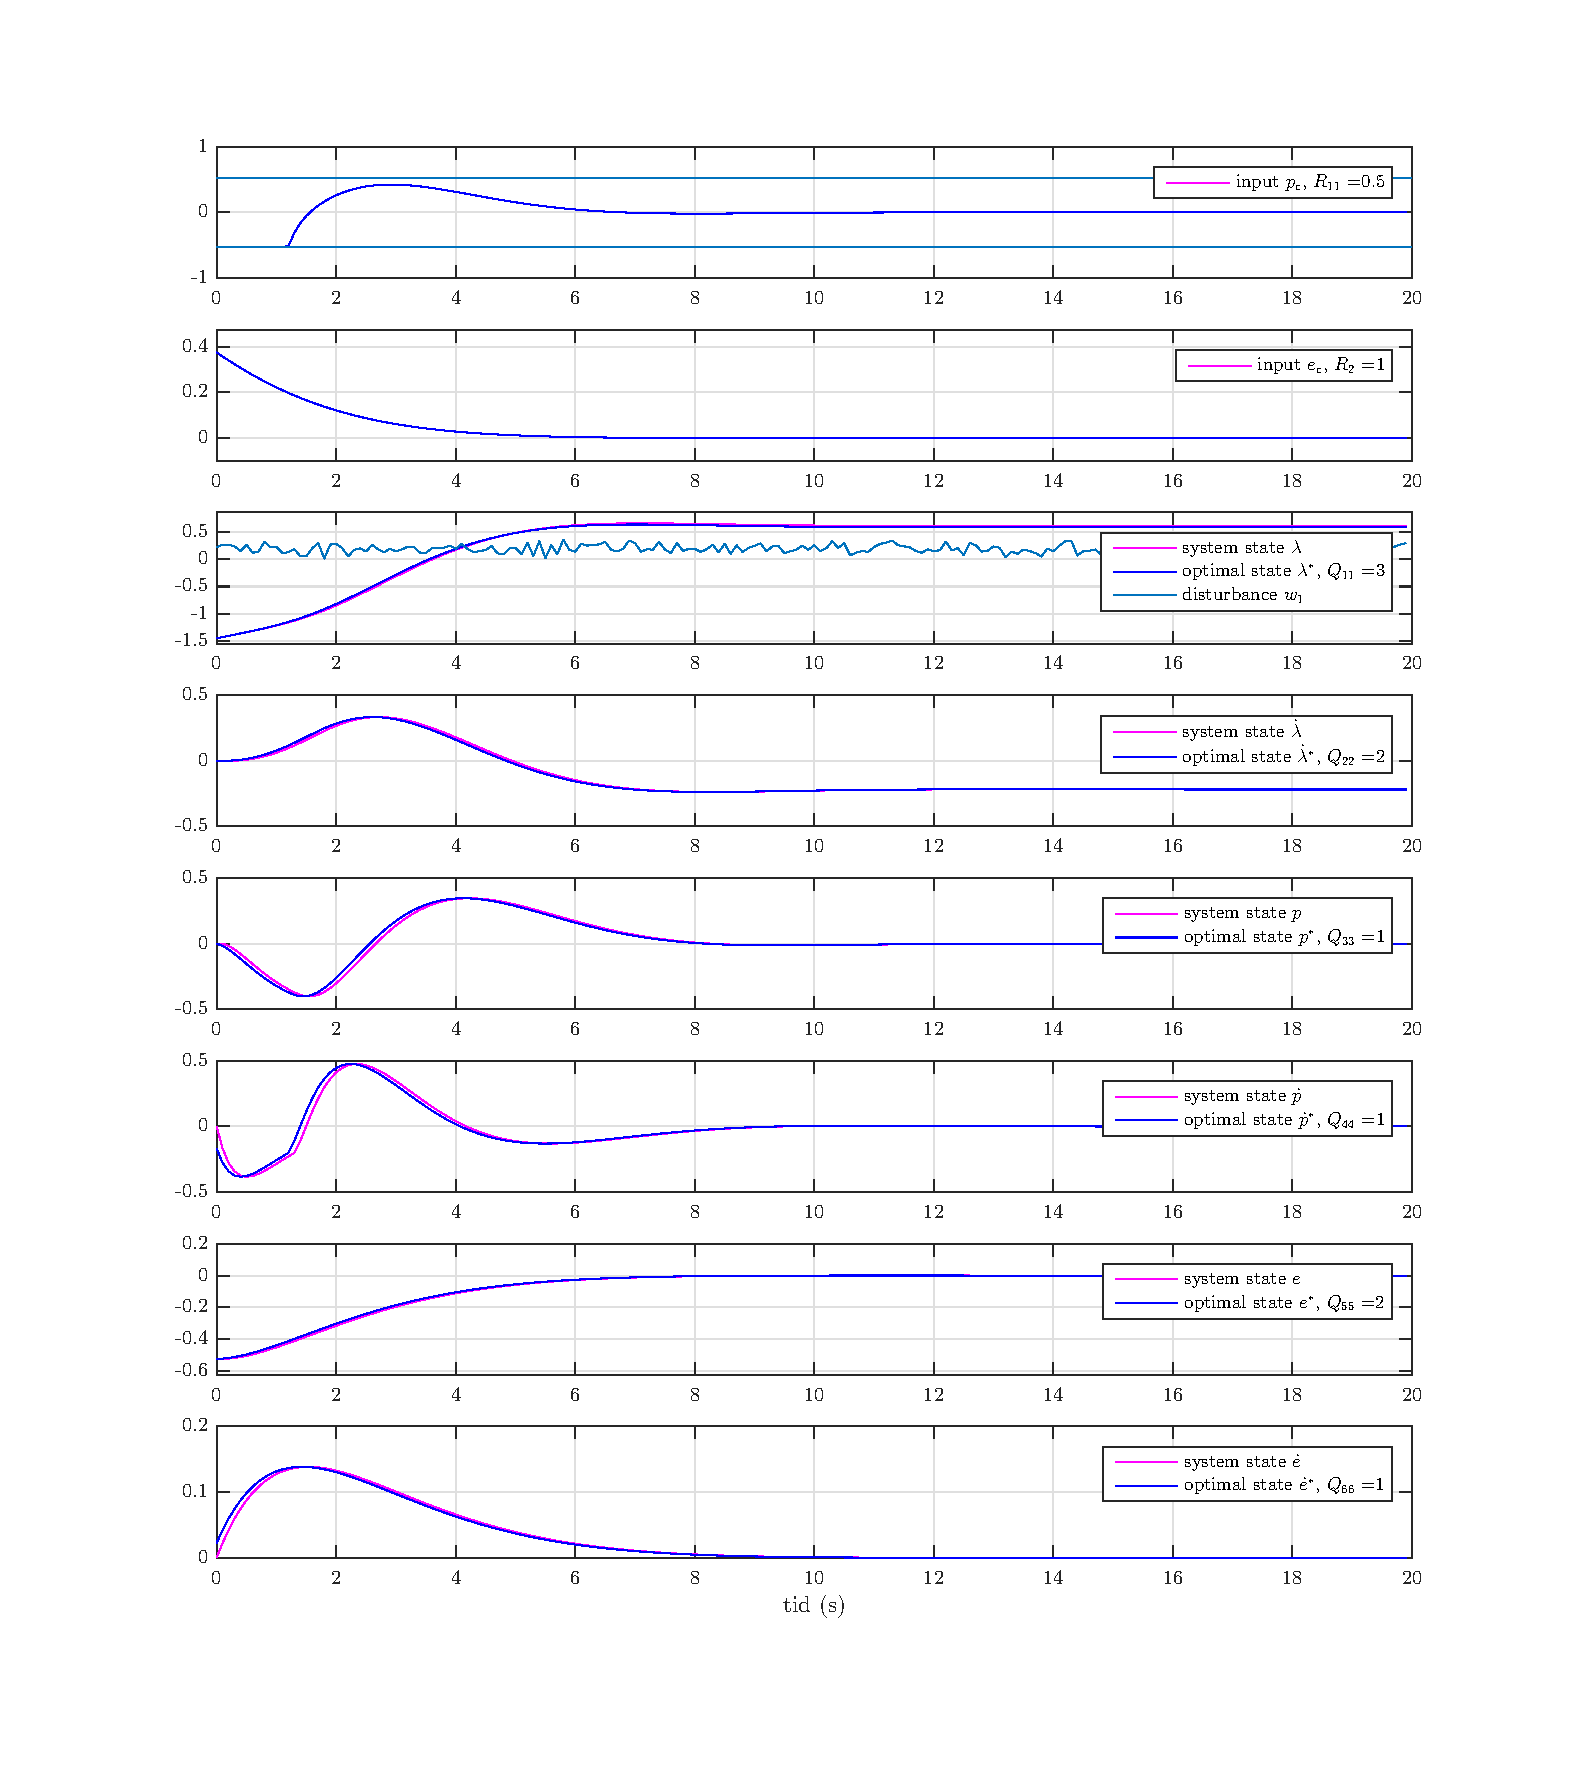
\includegraphics[scale=0.4]{fig/heli_sim_no_est_stable.eps}
    \caption{Simulation in MATLAB with stable \acrshort{mpc}}
    \label{fig:my_label}
\end{figure}

The value of $\lambda$ after 15 seconds, tends towards $[0.6133, 0.6137]$.


Then the same simulation and \acrshort{mpc}, but with an estimator to estimate the constant disturbance to remove the deviation in travel.

\begin{figure}[h!]
    \centering
    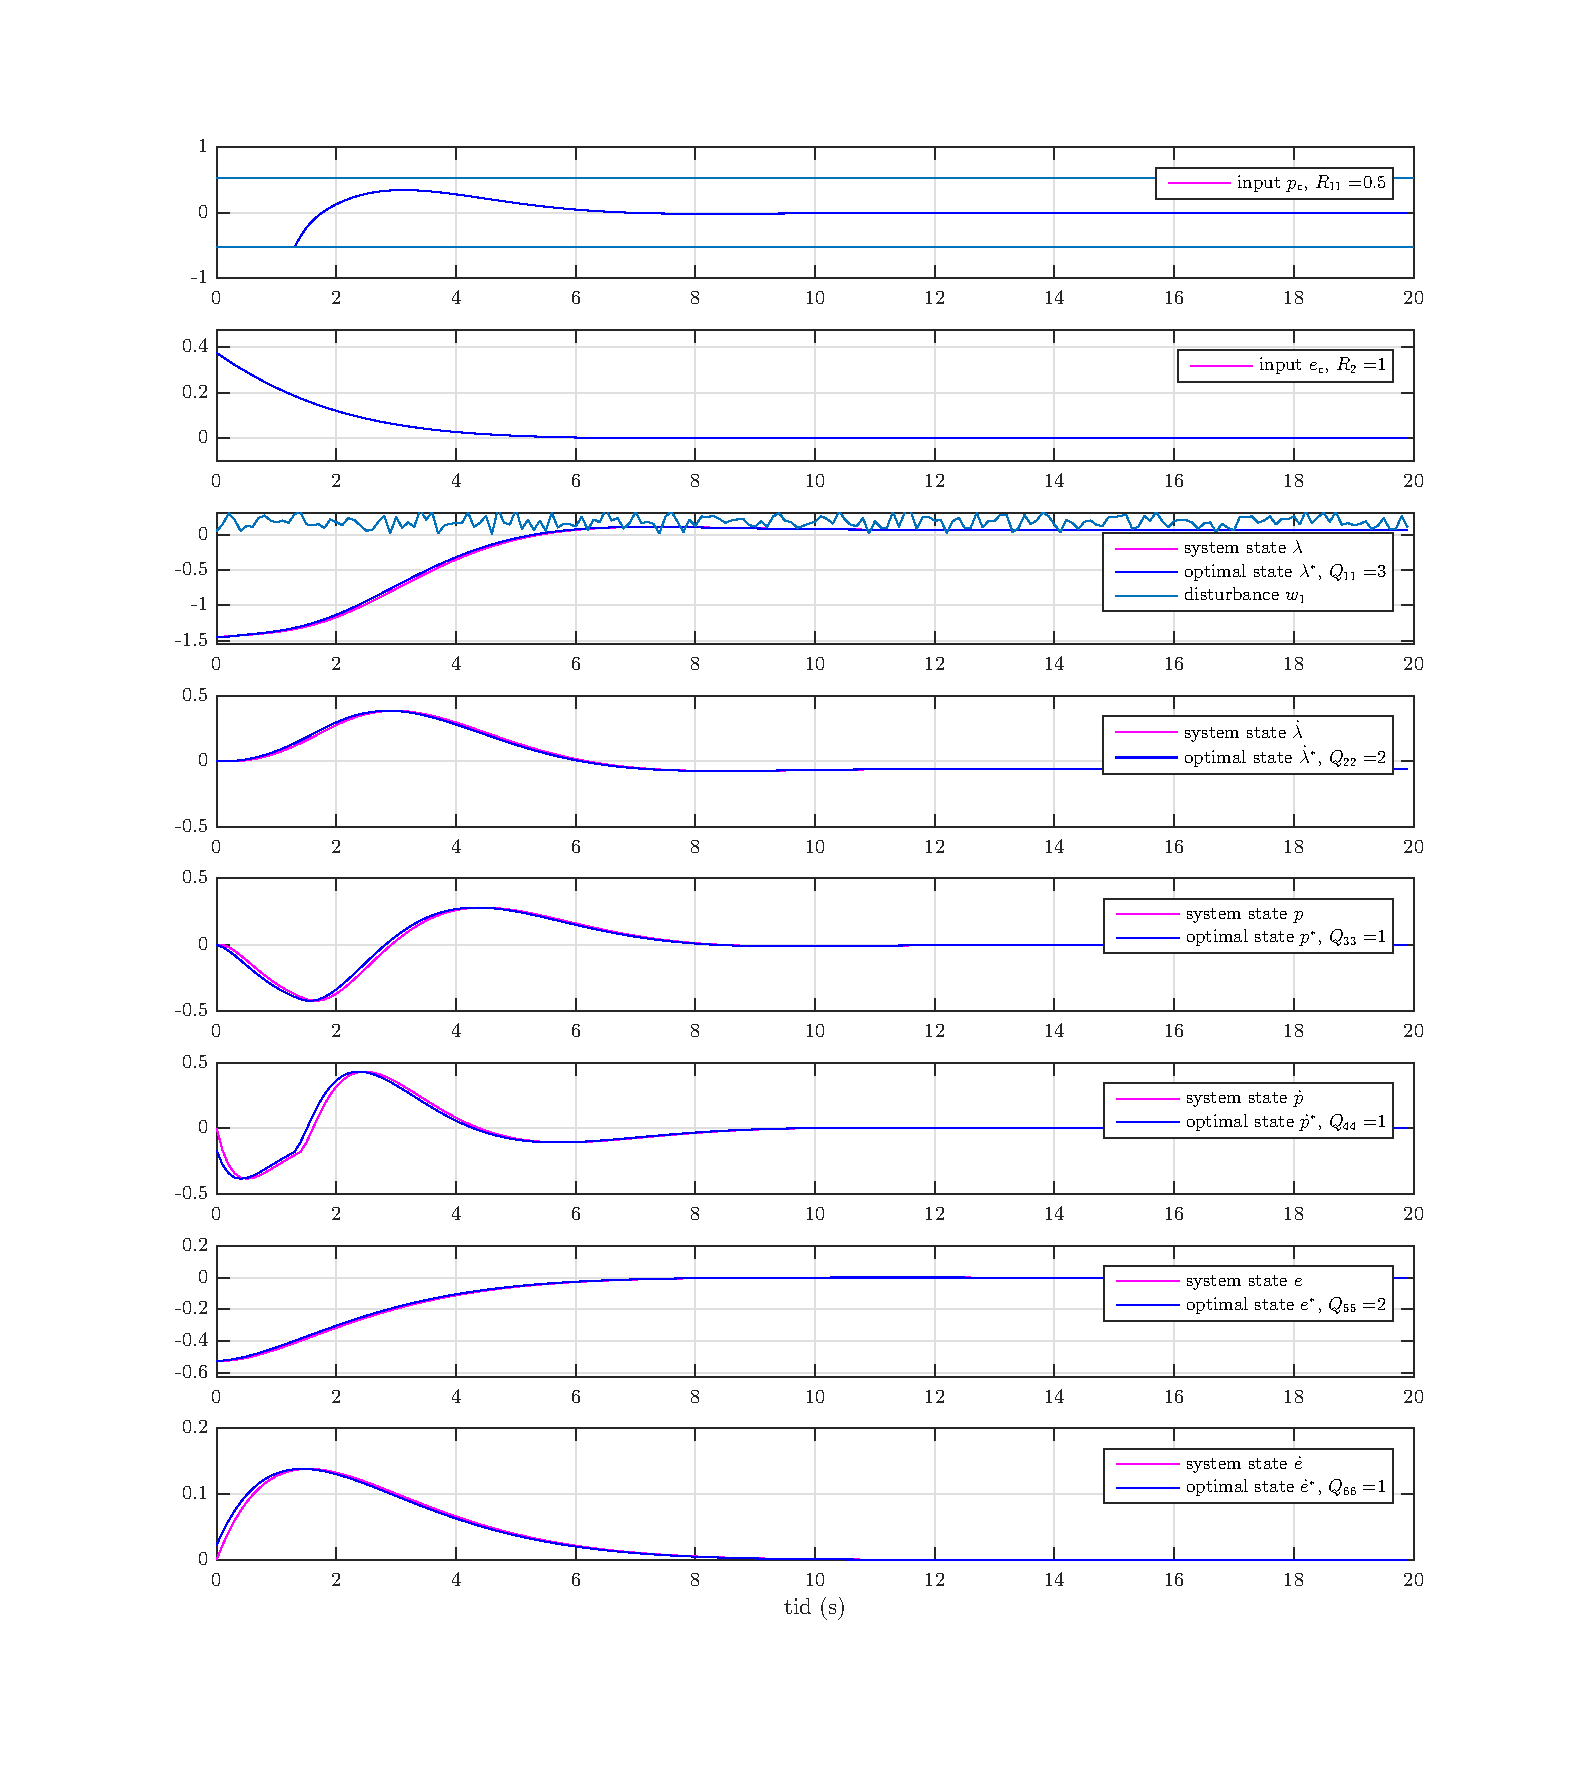
\includegraphics[scale=0.4]{fig/heli_sim_est_stable.eps}
    \caption{Simulation in MATLAB with stable \acrshort{mpc}}
    \label{fig:my_label}
\end{figure}

The value of $\lambda$ tends towards $[0.079]$.

%0.0787, 0.0791

Below is a plot of the error dynamics of the estimator, as well as the estimated disturbance $d$. 

\begin{figure}[h!]
    \centering
    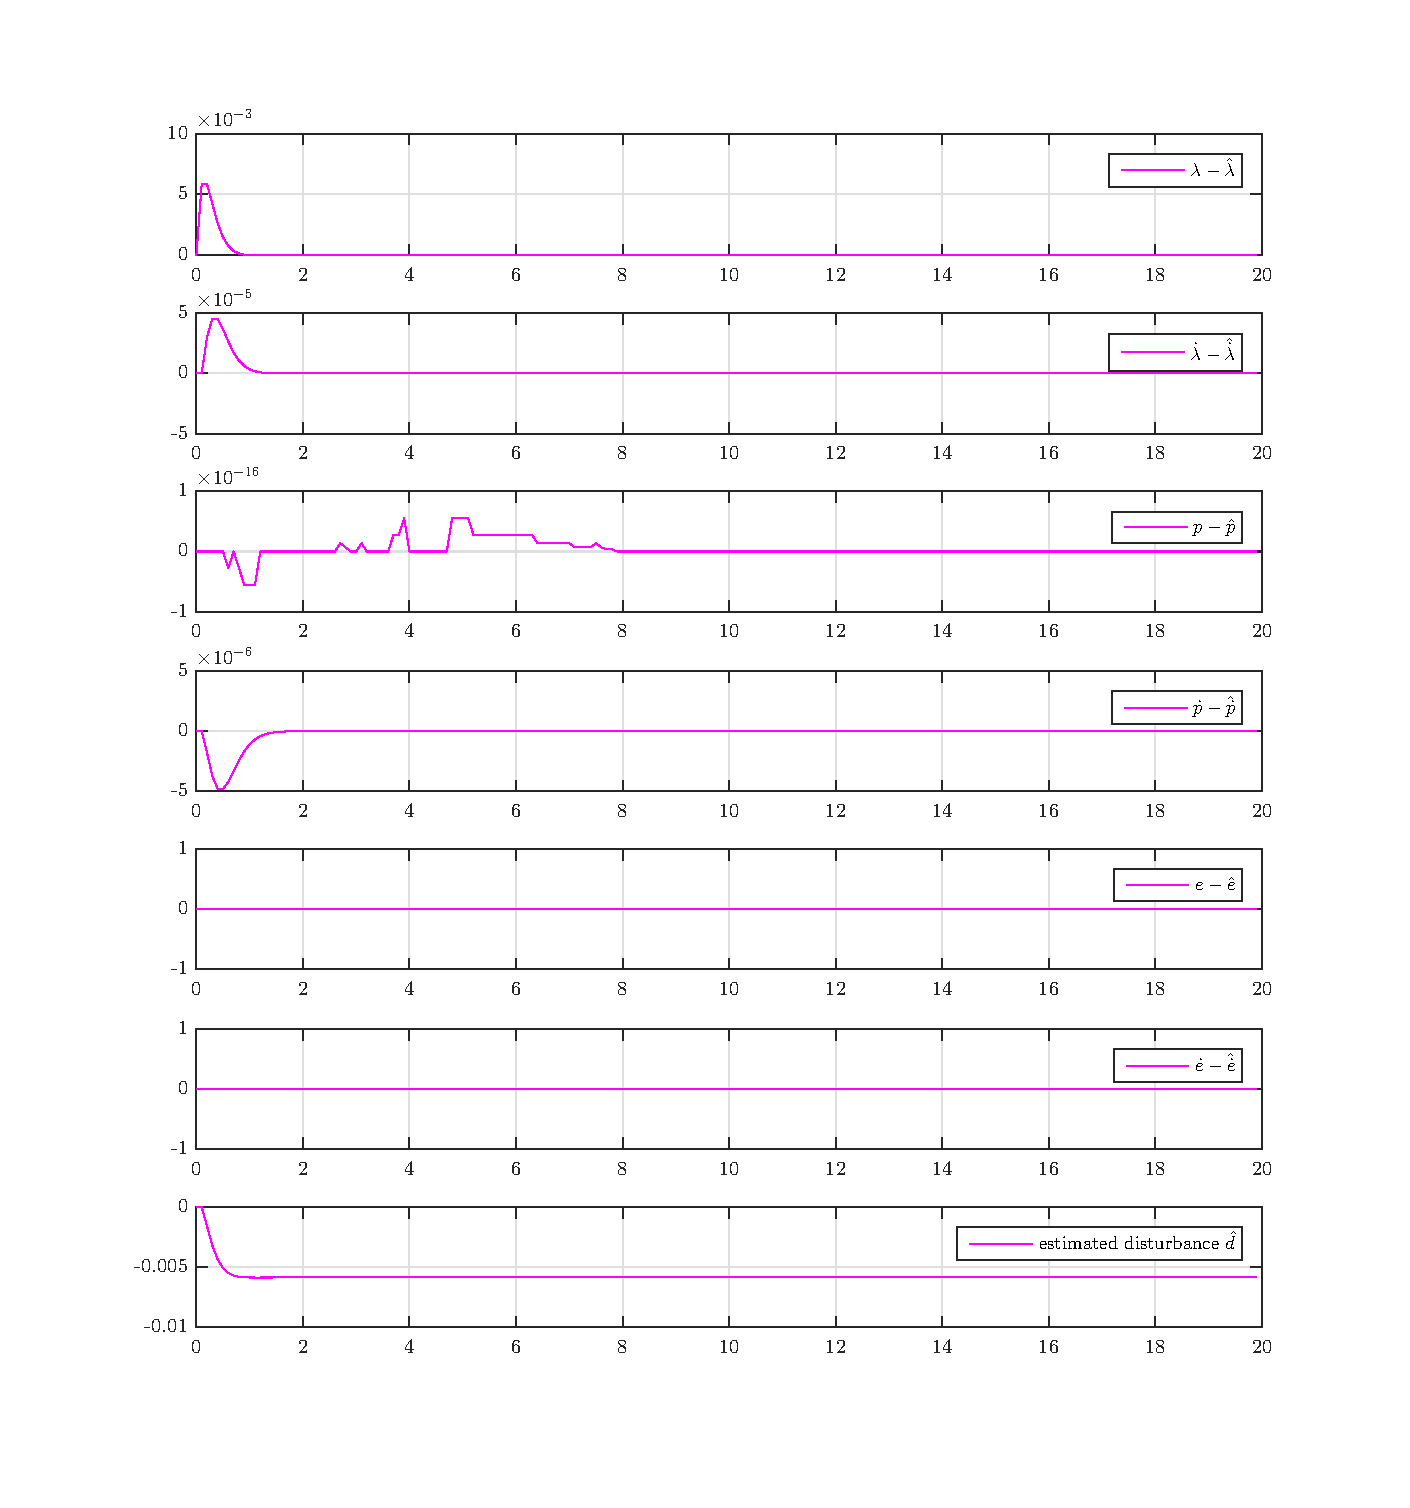
\includegraphics[scale=0.5]{fig/heli_sim_est_stable_error_plot.eps}
    \caption{Error dynamics of stable \acrshort{mpc}}
    \label{fig:my_label}
\end{figure}



\section{Helicopter performance in real time }



Both stable \acrshort{mpc} and unstable \acrshort{mpc}

And no offset as well

This section will demonstrate the effect the frequency of the \acrshort{mpc} has on the performance of the system, and how the frequency was selected. 

What factors come in to play when choosing the optimal frequency for the \acrshort{mpc} to run at.

The model will be run with a frequency of 12.5 Hz, 10 Hz and 5 Hz while the rest of the system will remain on 50 Hz. 

The optimization horizon is 15 in all of these. 
 intervals. 

\begin{figure}
    \centering
    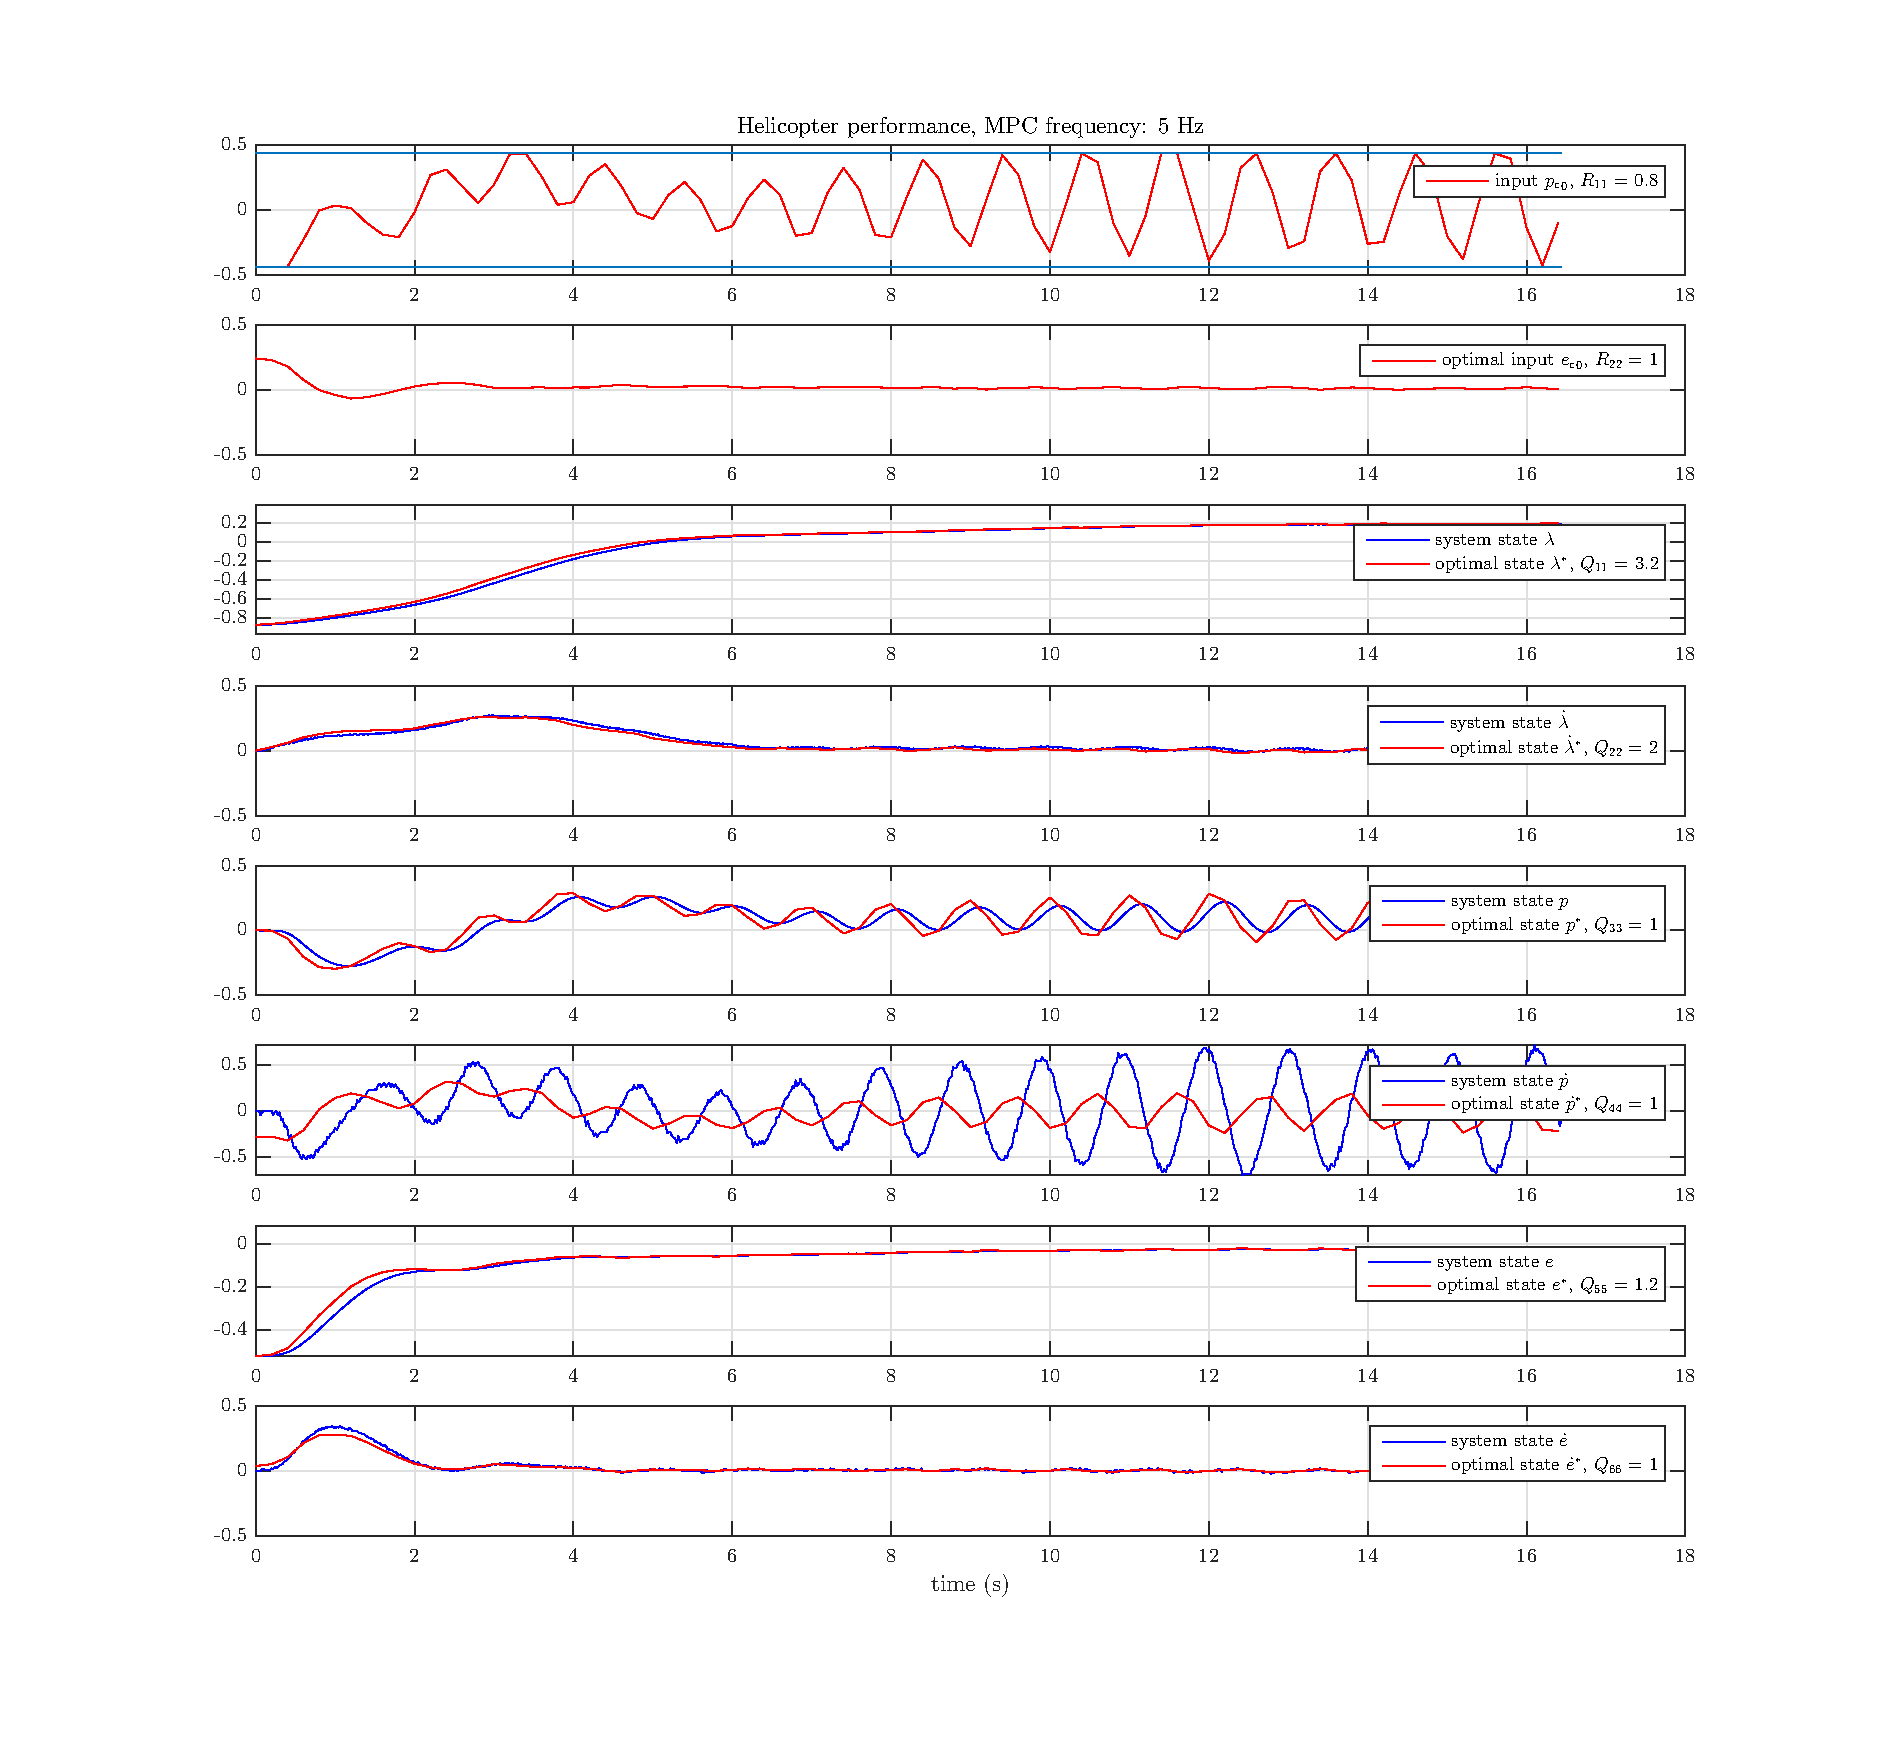
\includegraphics[scale=0.43]{fig/heli_sim_5_15_tune_2.eps}
    \caption{Helicopter performance with \acrshort{mpc} frequency 5 Hz}
    \label{fig:heli_sim_5_1}
\end{figure}


\begin{figure}
    \centering
    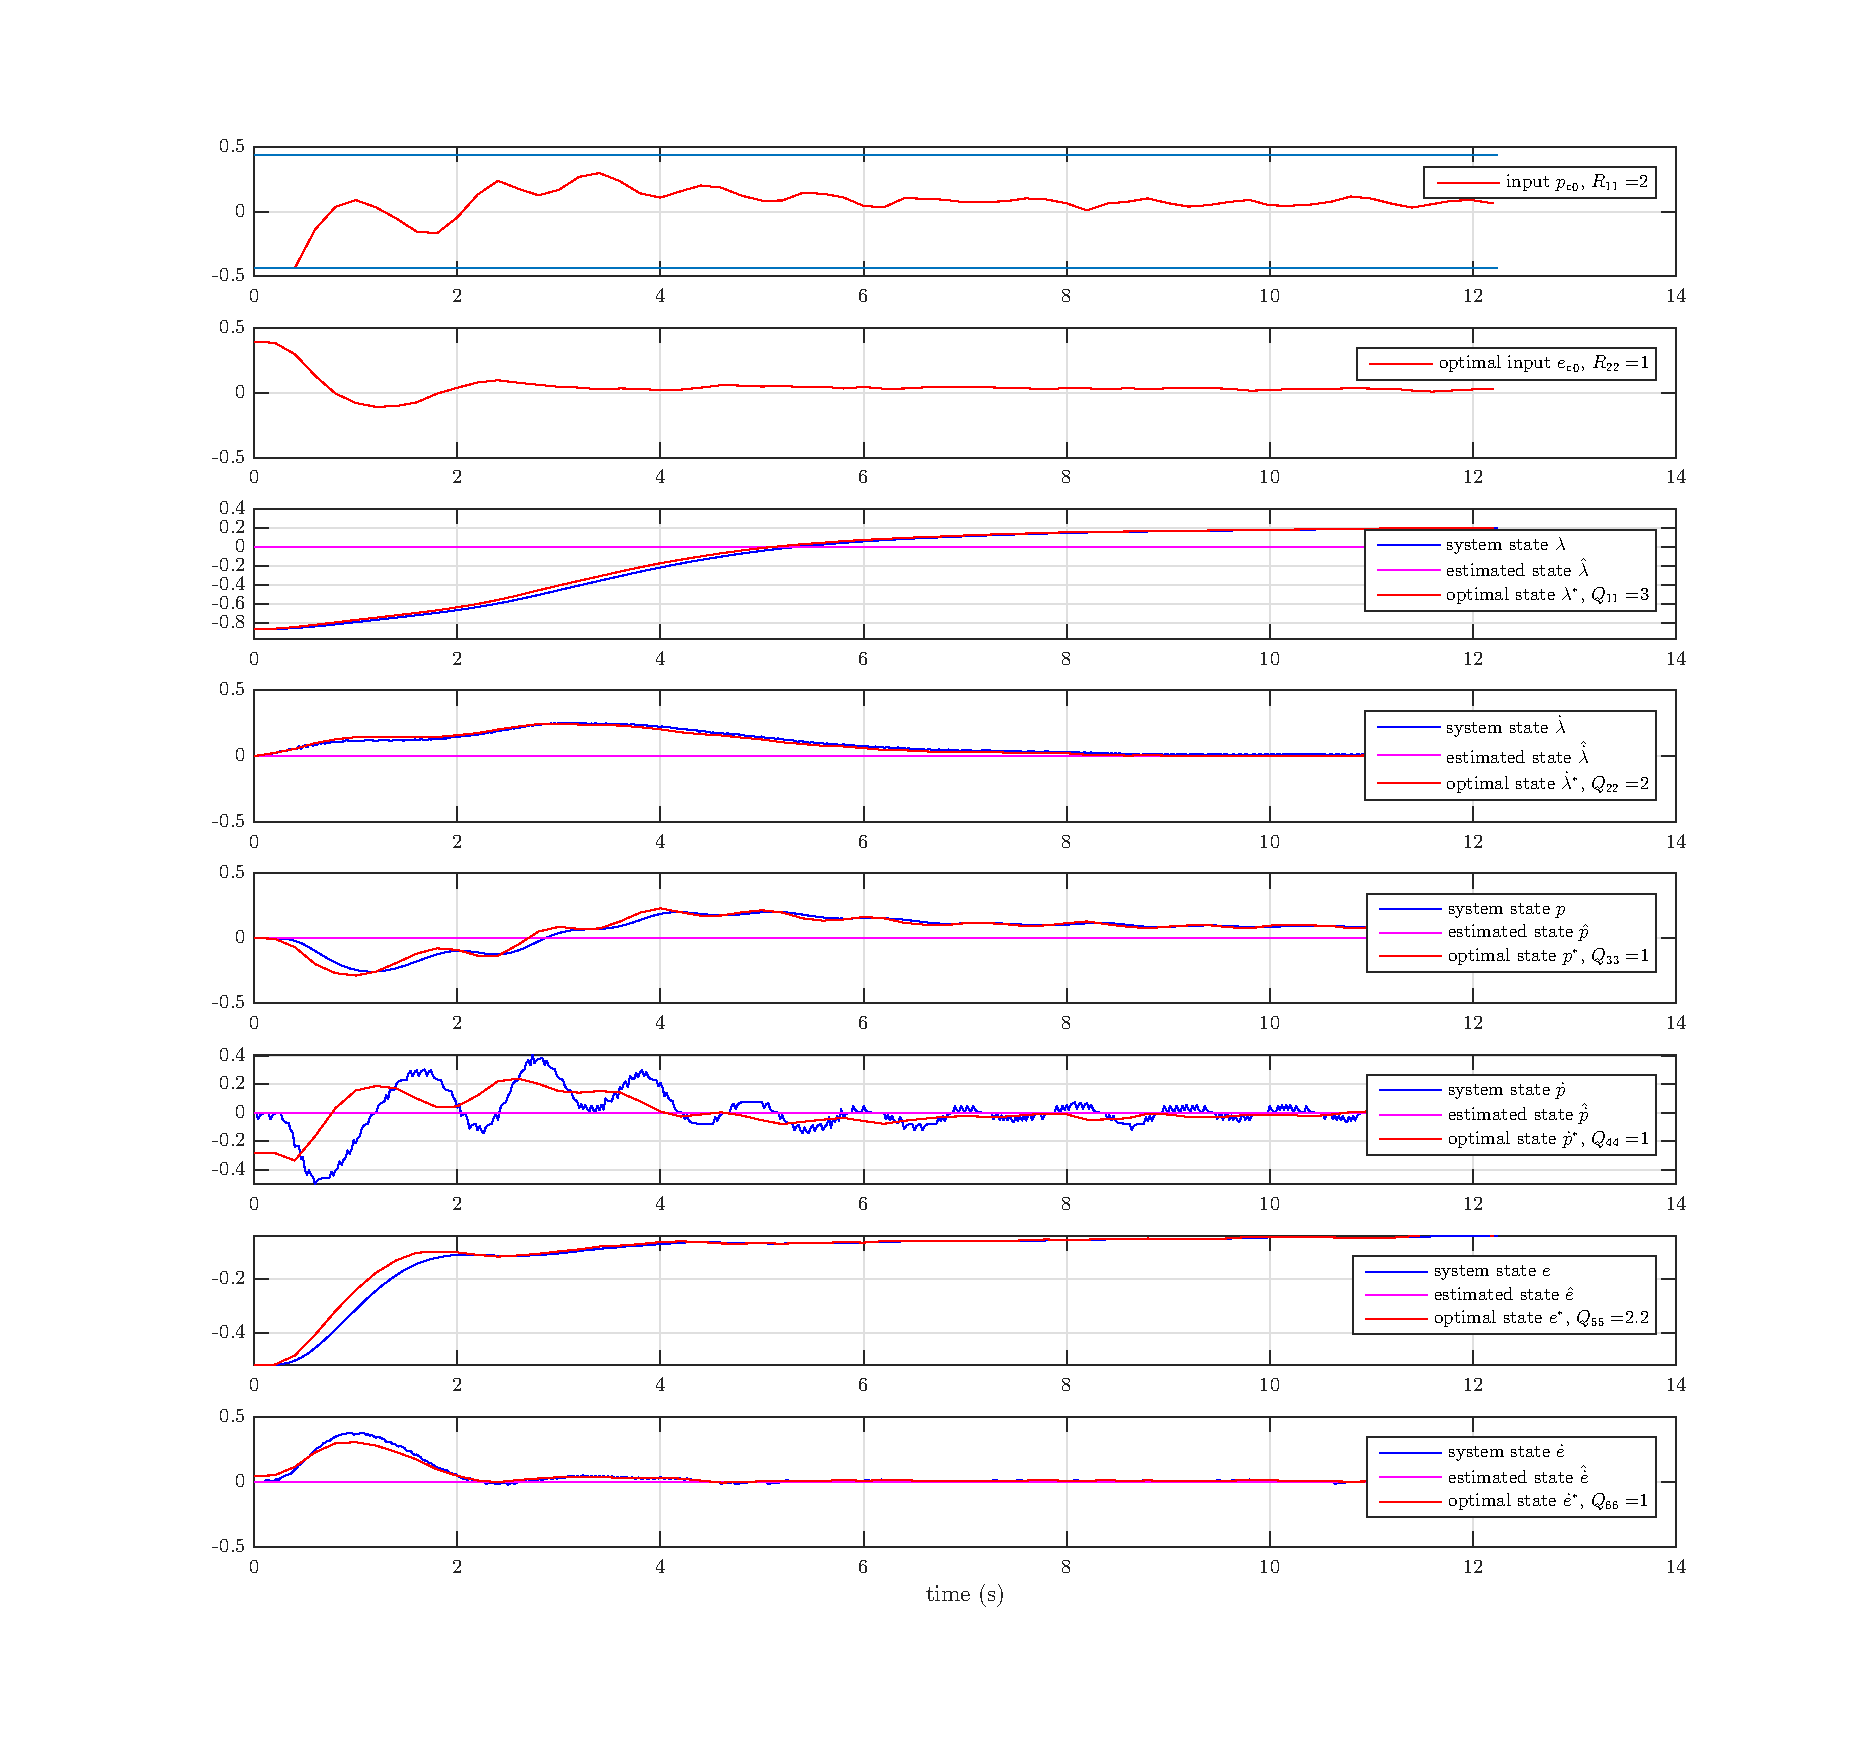
\includegraphics[scale=0.43]{fig/heli_sim_5_15.eps}
    \caption{Helicopter performance with \acrshort{mpc} frequency 5 Hz}
    \label{fig:heli_sim_5_2}
\end{figure}

\begin{figure}
    \centering
    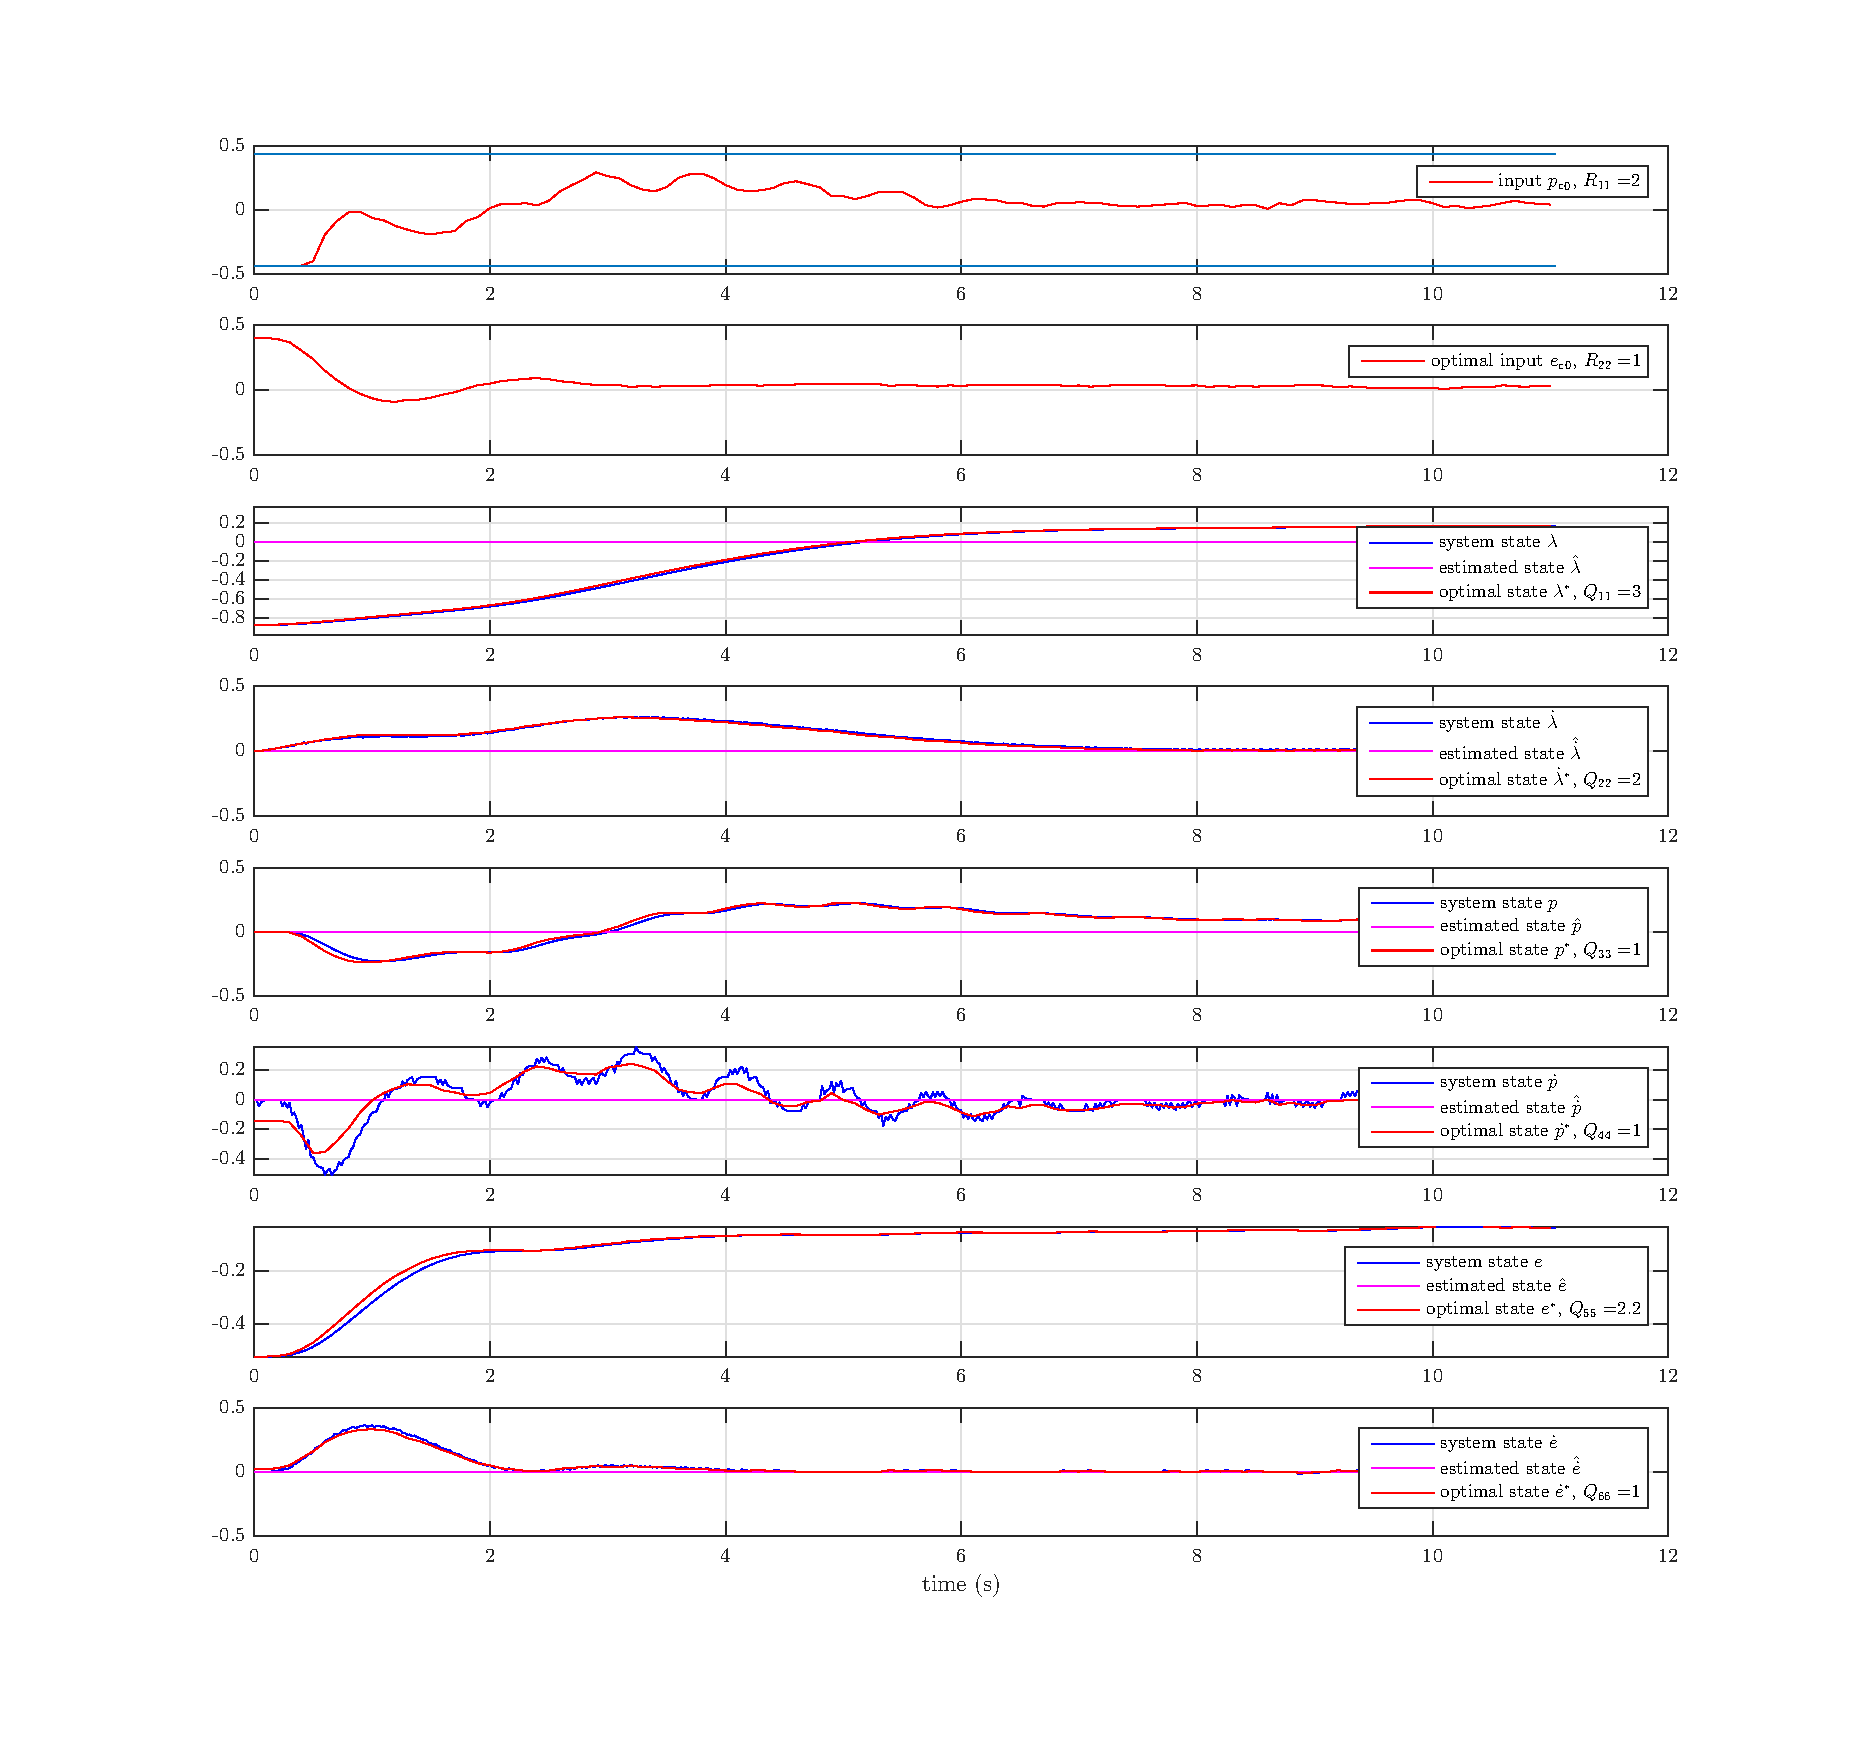
\includegraphics[scale=0.43]{fig/heli_sim_10_15.eps}
    \caption{Helicopter performance with \acrshort{mpc} frequency 10 Hz}
    \label{fig:heli_sim_10_1}
\end{figure}

\begin{figure}
    \centering
    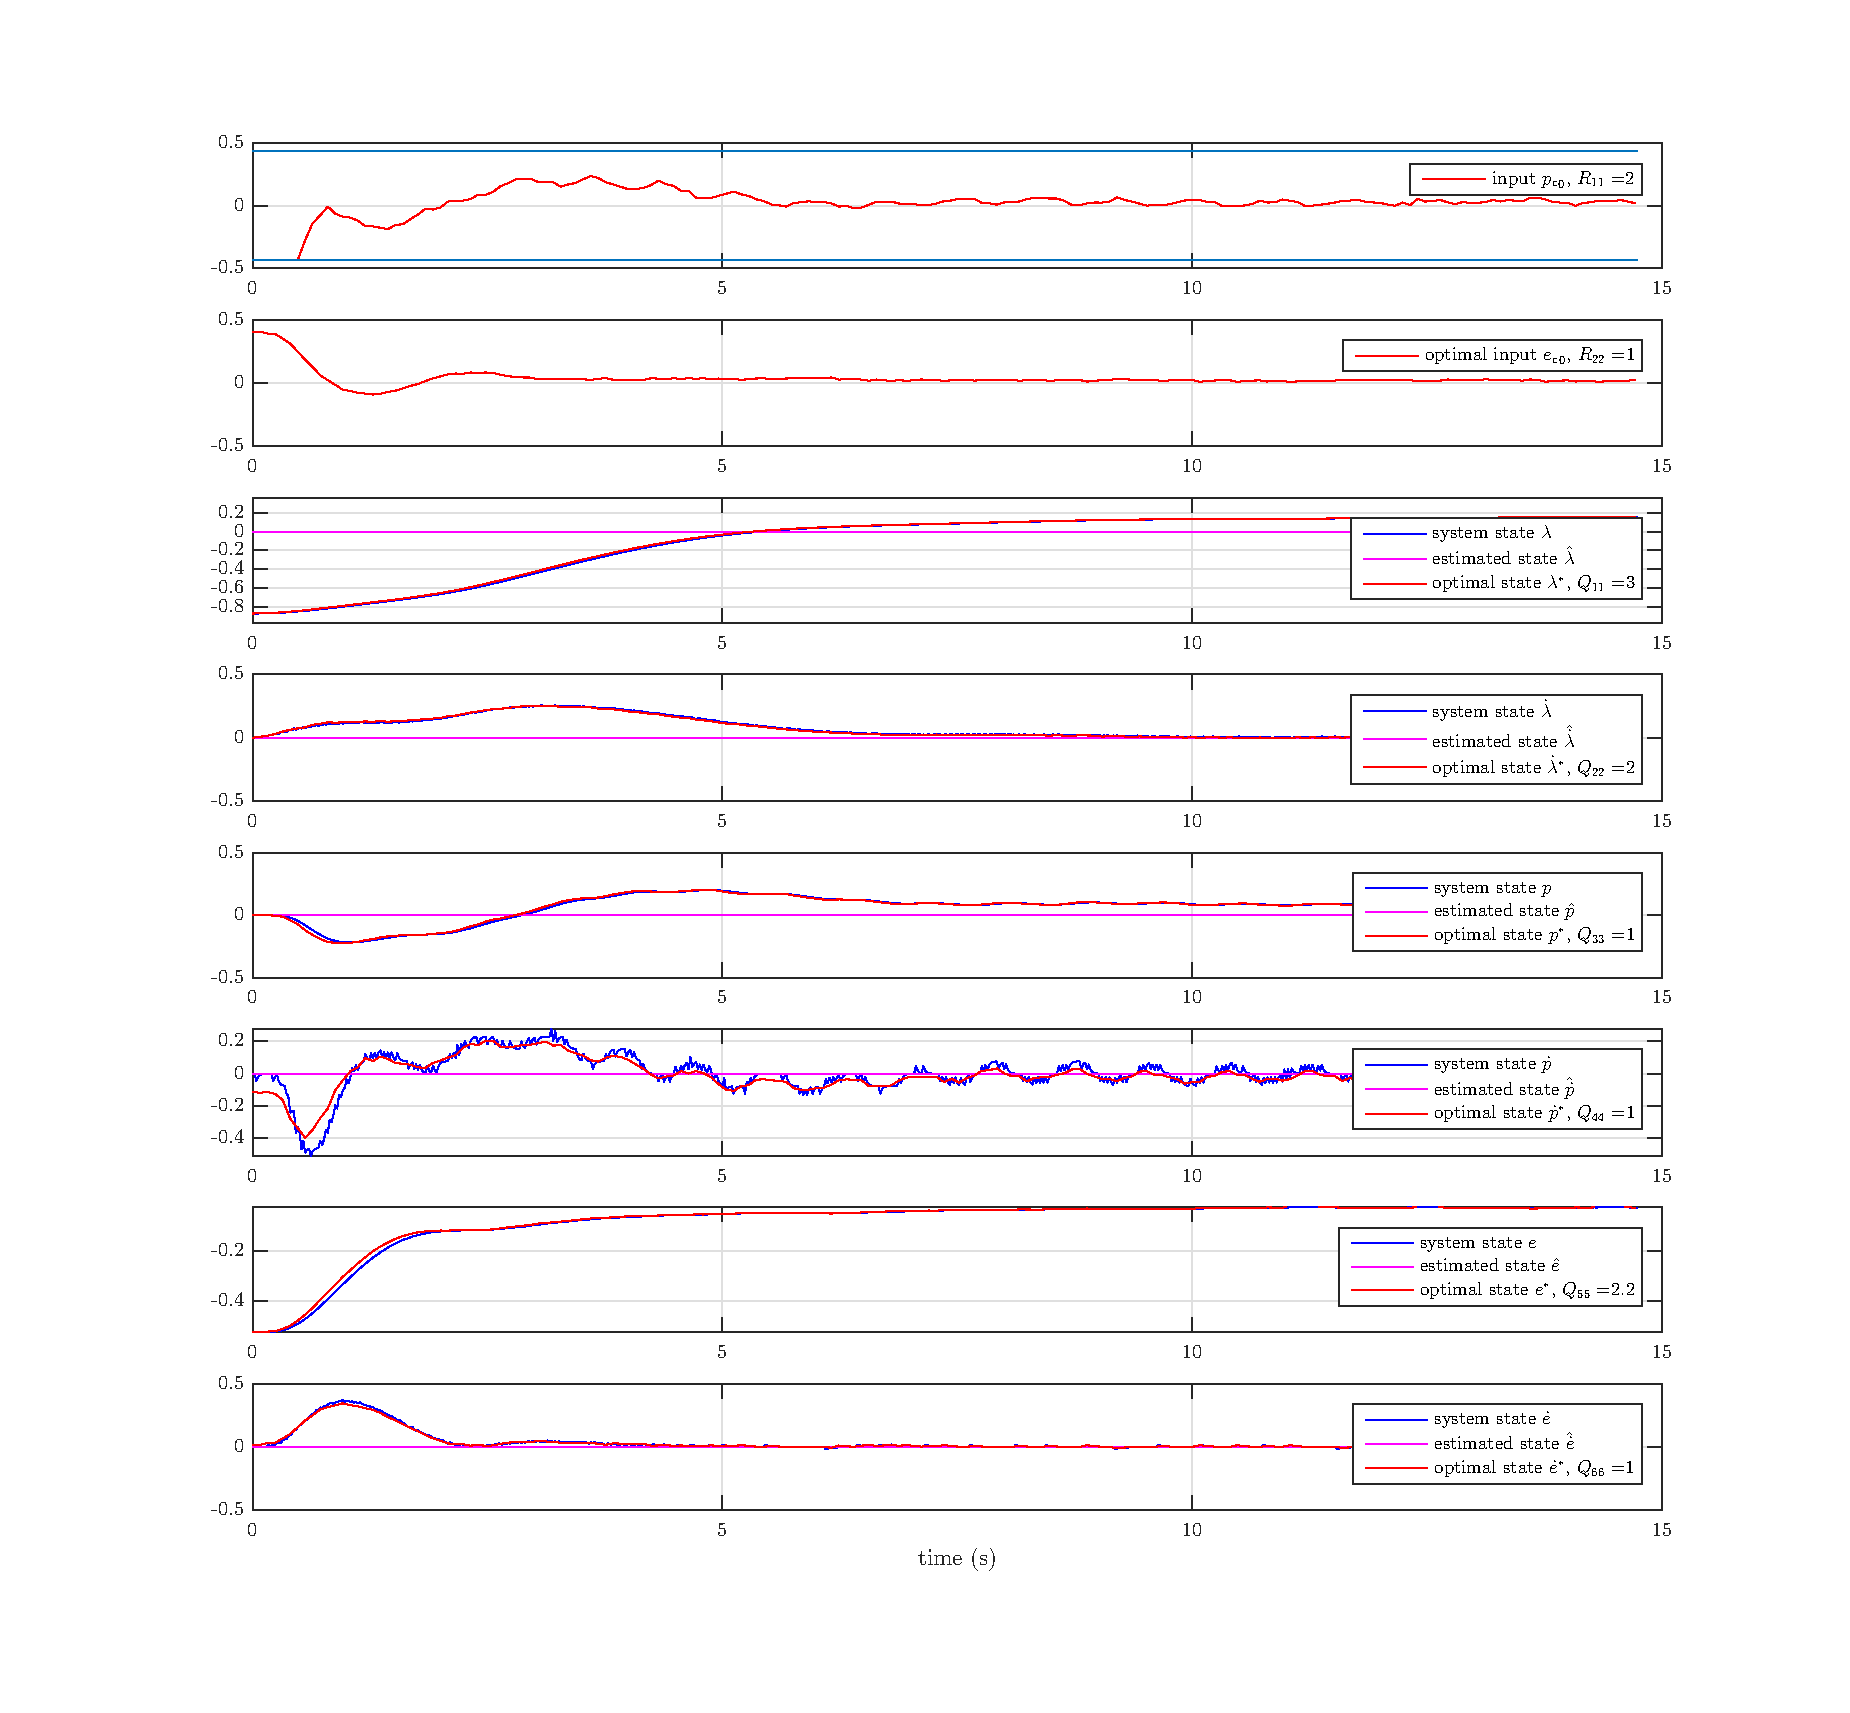
\includegraphics[scale=0.43]{fig/heli_sim_125_15.eps}
    \caption{Helicopter performance with \acrshort{mpc} frequency 12.5 Hz}
    \label{fig:heli_sim_125_1}
\end{figure}

\begin{figure}
    \centering
    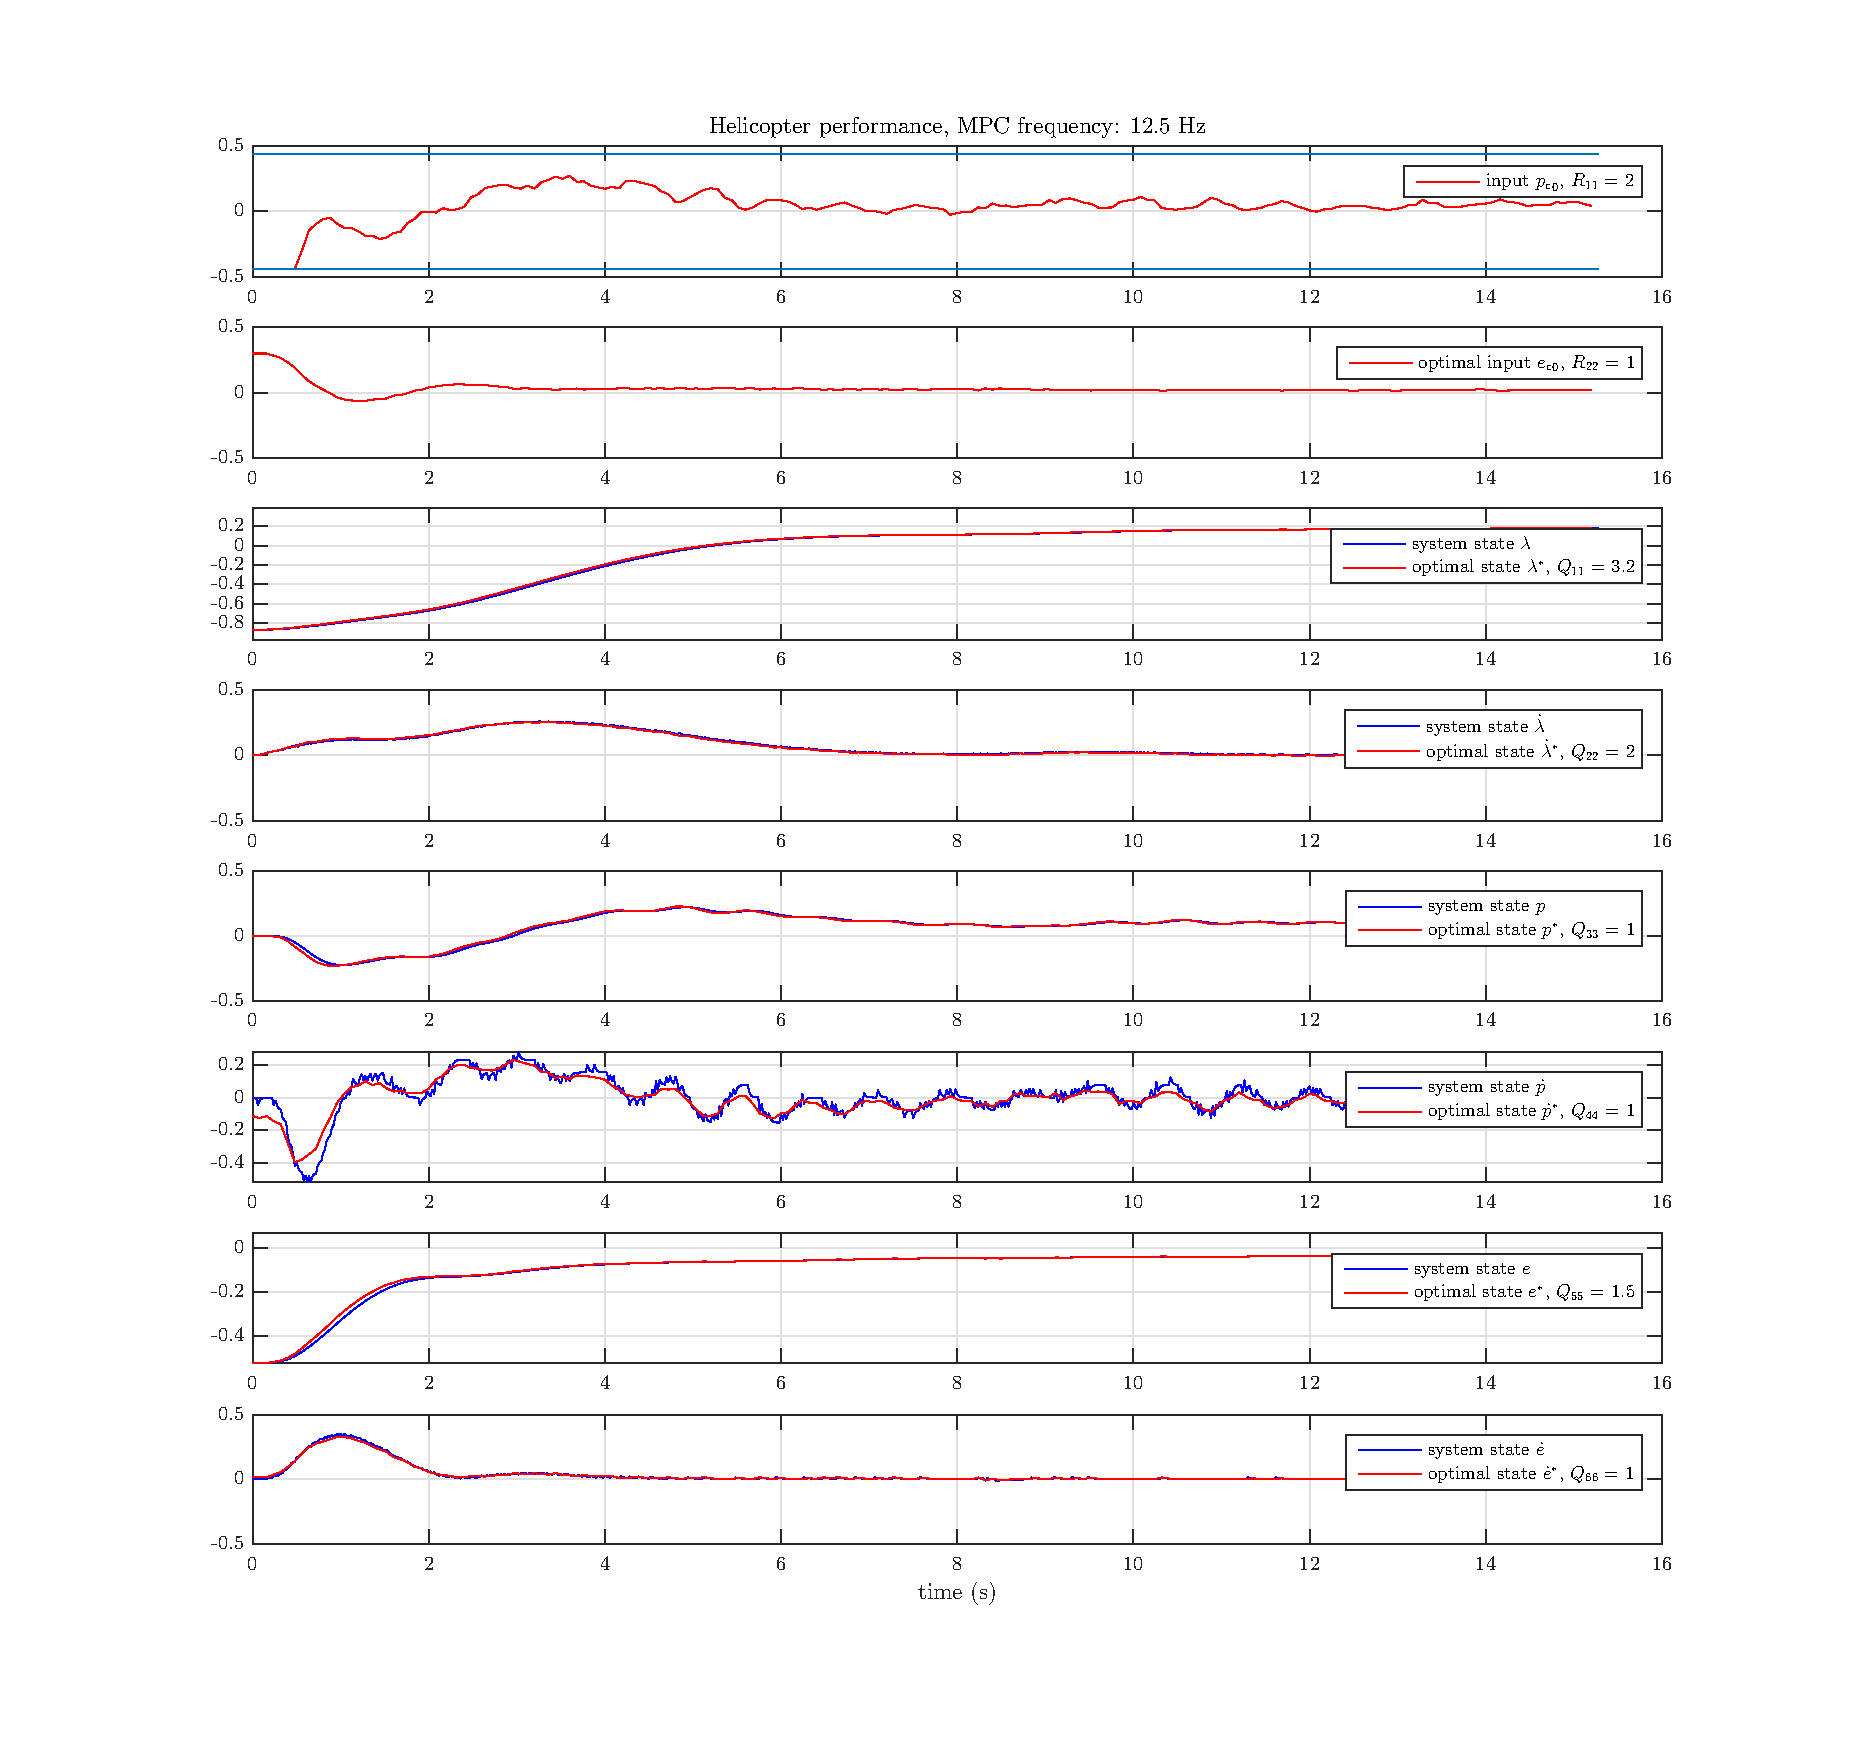
\includegraphics[scale=0.43]{fig/heli_sim_125_15_tune_3.eps}
    \caption{Helicopter performance with \acrshort{mpc} frequency 12.5 Hz}
    \label{fig:heli_sim_125_2}
\end{figure}


\section{OSQP performance}






%DISCUSSION
\chapter{Discussion}\label{ch:discussion}

The effects of adding a terminal cost and terminal constraint are clearly demonstrated from the performance of the simulation. The system is much more stable, and approaches the equilibrium point much faster. In addition, the constant deviation that is present because of the disturbance is not as large when controlled with stable \acrshort{mpc}. 

\section{Performance of nominal MPC}

It is beneficial for the \acrshort{mpc} to have a low frequency, as this results in a computationally inexpensive system because the optimization problem has to be solved less often. However, there is a trade-off. A lower frequency gives any model discrepancies or any disturbances time to develop before the \acrshort{mpc} receives a new state and calculates a new control input. 

Consider the unconstrained \acrshort{mpc}, which is just an \acrshort{lqr} regulator, much like a \acrshort{pd}-controller. The low frequency equates to a higher time delay. 

For this case, a highly non-linear system has been linearized about the equilibrium point, so non-linearities will occur when the states move away from this point. 

The first run of the helicopter, shown in figure \ref{fig:heli_sim_5_1} shows this very well. Because the feedback to the helicopter is at a much lower rate than the rest of the system (ten times slower), the non-linearities on the system have time to develop before the \acrshort{mpc} receives updated information and calculates a new input. This explains the heavy oscillations one can see in both the pitch reference, the pitch and pitch rate. 

An attempted solution to this problem, seen in figure \ref{fig:heli_sim_5_2} is too tune the \acrshort{mpc} by increasing the oscillating control inputs weight. It is apparent that this works to some degree, the oscillation nearly disappears.

However, to decrease the time it takes for the helicopter to reach its designated target one might consider just increasing the frequency of the \acrshort{mpc}. 

Figure \ref{fig:heli_sim_10_2} shows this. 

Another consideration point when choosing the frequency is the fact that the system model used in the \acrshort{mpc} has to be discretized with the sampling interval $T = \frac{1}{f_{\text{MPC}}}$, where $f_{\text{MPC}}$ is the frequency for the \acrshort{mpc}. This means that for larger frequencies the same control horizon $N = 15$, becomes shorter in the mind of the \acrshort{mpc}. This leads to infeasibility problems.

Consider the system starting at $\lambda = 180 deg$ and trying to move to $0$. The terminal constraint imposed on the last state of the optimal state trajectory requires the system being able to be near the equilibrium point in 15 steps. When the actual time of these 15 steps decreases, because the system model is discretized with a smaller value, the starting point of the system yields an infeasible control problem. 

So larger frequency limits the initial values of the system. 

\section{Performance of stable MPC}
Discuss first the effect of adding the P and the terminal constraint.

\subsection{With state estimation}
Discuss the effect of modeling the disturbance

It is clear from the Simulation in MATLAB that modelling the disturbance was successful in removing the constant offset in the travel. However, when running the same on the helicopter, the results varied.



\section{Performance of OSQP}

Discuss the OSQP performance. Compare it to other popular embedded \acrshort{qp}-solvers (fast gradient method?)

\section{Future work}

The potential extensions to this project are endless. Upgrading the estimator from a Luenberger observer to a Kalman filter is a good start. This requires some testing of the system, to find the covariance value of the disturbance. However, it is obvious that the better estimation of the disturbance, the easier it is to account for.

Some other exciting this that can be done is adding a reference signal into the \acrshort{mpc} block. Potentially a time-varying signal such as the sinus curve, which is a block in Simulink. 

The other obvious extension to this project is using nonlinear model predictive control. Obviously the system in question is highly non-linear so implementing a nonlinear controller would yield much more accurate results. 

Another potential improvement, is implementing a form of \acrshort{mpc} that accounts for disturbance such as for example tube-based \acrshort{mpc}. This will help with the offset in travel, and could also help with the inaccurate model if one can find a way to model the non-linearities as disturbances. However, most likely, nonlinear \acrshort{mpc} is the best solution.




%CONCLUSION
\chapter{Conclusion}

The research question for this thesis was in short \textit{What are the effects of controlling a 3 DOF helicopter using linear \acrlong{mpc}?}

Conclusively, using \acrshort{mpc} to control a propeller under-actuated system such as the Quanser's 3 DOF Helicopter is both a useful area of research, and it also showed a few things. 

The performance difference between linear \acrlong{mpc} with and without the terminal cost and constraint was very apparent in this system. In addition, the attempt to remove the offset by modelling the constant disturbance was relatively successful. 

The work done on this piece of equipment is extensive, and the work presented here will only add to that. 

Going forward, adding trajectory tracking would be a natural next step. Nonlinear \acrlong{mpc} could also have some interesting application, both academically and for application to larger, more complex systems. In addition, it is apparent that robust control of the system is needed, as there a many disturbances that are not modelled here. Robust linear control would be less complex than non-linear control, where there would still be disturbances that are not modelled. 

\newpage

%ACRONYMS
\printglossary[title=Acronyms, toctitle=Acronyms, type=\acronymtype]

%BIBLIOGRAPHY

\addcontentsline{toc}{chapter}{Bibliography}

\bibliographystyle{elsarticle-harv}
\bibliography{mylib}

\cleardoublepage

\pagenumbering{gobble}

%APPENDIX
\begin{appendices}
\appendixpagenumbering


\chapter{System parameters}

\begin{table}[tbp]
	\centering
	\caption{Parameters and values.}
	\begin{tabular}{llll}
		\toprule
		Symbol & Parameter & Value & Unit \\
		\midrule
		$l_a$ & Distance from elevation axis to helicopter body & $0.63$  & m               \\
		$l_h$ & Distance from pitch axis to motor               & $0.18$  & m               \\
		$K_f$ & Force constant motor                            & $0.25$  & N / V            \\
		$J_e$ & Moment of inertia for elevation                 & $0.83$  & kg ${\text{m}^2}$ \\
		$J_t$ & Moment of inertia for travel                    & $0.83$  & kg ${\text{m}^2}$ \\
		$J_p$ & Moment of inertia for pitch                     & $0.034$ & kg ${\text{m}^2}$\\
		$m_h$ & Mass of helicopter                              & $1.05$  & kg              \\
		$m_w$ & Balance weight                                  & $1.87$  & kg              \\
		$m_g$ & Effective mass of the helicopter                & $0.05$  & kg              \\
		$K_p$ & Force to lift the helicopter from the ground    & $0.49$  & N               \\
		\bottomrule
	\end{tabular}
\label{tab:parameters}
\end{table}


\chapter{Simplification of helicopter model}\label{ch:linear_heli_model}


The linear approximation of the function $y = f(x,u)$ about $(x^*, u^*)$ using the first-order Taylor series and defining the new states $\Delta x = (x - x^*), \Delta u = (u-u^*)$ is defined as, 

\begin{equation}\label{eq:lin_approx}
    \begin{split}
        y &\approx f(x^*, u^*) + \frac{\partial f }{\partial x}|_{(x^*, u^*)} \Delta x + \frac{\partial f}{\partial u}|_{(x^*, u^*)} \Delta u \: \: .\\
    \end{split}
\end{equation}

Given the non-linear equations of motions of the helicopter system,
\begin{equation}
    \begin{split}
        \ddot \lambda &= -\frac{1}{J_{\lambda}}(L_3 V_s \cos e \sin p) \: \: , \\
        \ddot p &= \frac{L_1 V_d}{J_p} \: \: , \\
        \ddot e &= -\frac{1}{J_e}(L_2 \cos e + L_3 V_s \cos p) \: \: ,\\ 
    \end{split}
\end{equation}

the linear approximation described above can be used to obtain a linear approximation, which is needed for the \acrshort{mpc}-problem. 

In addition, the resulting linear system should be a first-order system, so let the states be 
\begin{equation}
    x^\top = \m{\lambda & \dot \lambda & p & \dot p & e & \dot e} \: \: ,
\end{equation}
while the inputs are 
\begin{equation}
    u^\top = \m{V_s & V_d} \: \: .
\end{equation}



\begin{equation}
    \dot x = f(x,u) = \m{\dot \lambda \\ -\frac{1}{J_{\lambda}}(L_3 V_s \cos e \sin p) \\ \dot p \\ \frac{L_1 V_d}{J_p} \\ \dot e \\ -\frac{1}{J_e}(L_2 \cos e + L_3 V_s \cos p } \: \: .
\end{equation}

The equilibrium point of the system $x^* = 0, \dot x^* = 0, \ddot x^* = 0$. This results in the input $V_s^* = -\frac{L_2}{L_3}, V_d^* = 0$. The resulting linearization becomes

\begin{equation}
    \begin{split}
        \dot x &= Ax + Bu \: \:  \\
         A &= \m{0 & 1 & 0 & 0 & 0 & 0 \\
              0 & 0 & \frac{L_2}{J_{\lambda}} & 0 & 0 & 0 \\
              0 & 0 & 0 & 1 & 0 & 0 \\
              0 & 0 & 0 & 0 & 0 & 0 \\
              0 & 0 & 0 & 0 & 0 & 1 \\
              0 & 0 & 0 & 0 & 0 & 0}, \: \: B = \m{0 & 0 \\
              0 & 0 \\
              0 & 0 \\
              0 & \frac{L_1}{J_p} \\
              0 & 0 \\
              \frac{L_3}{J_e} & 0} \: \: .
    \end{split}
\end{equation}

This is the lowest level of control. On top of this, a PD and a PID controller are added to control the pitch and elevation respectively.

\begin{equation}
    \begin{split}
        V_d = K_{pp} (p_c - p) - K_{pd} \dot p \\
        V_s = K_{ep}(e_c - e)  - K_{ed} \dot e
    \end{split}
\end{equation}

Let $u^\top = \m{p_c & e_c}$, and the  resulting first order \textit{discrete} linear system with time step $h$ is,
\begin{equation}
    \begin{split}
        \dot x &= Ax + Bu \: , \; \; \\
        A &= \m{1 & h & 0 & 0 & 0 & 0 \\
                0 & 1 & -hK_2 & 0 & 0 & 0 \\
                0 & 0 & 1 & h & 0 & 0 \\
                0 & 0 & -hK_1 K_{pp} & 1-hK_1 K_{pd} & 0 & 0 \\
                0 & 0 & 0 & 0 & 1 & h \\
                0 & 0 & 0 & 0 & -hK_3 K_{ep} & 1-hK_3 K_{ed}}, \\
        B &= \m{0 & 0 \\ 0 & 0 \\ 0 & 0 \\
                hK_1 K_{pp} & 0 \\ 0 & 0 \\ 0 & h K_3 K_{ep}} \: \: .
    \end{split}
\end{equation}


$J_e \ddot e = l_a K_f V_s - T_g.$
Mens jeg har 
$J_e \ddot e = -L_2 \cos e + L_3 V_s \cos p$




\chapter{MATLAB Code}

\begin{lstlisting}[caption={init.m}]]
% Updated spring 2018, Andreas L. Fl\r{a}ten
% Updated Spring 2019, Joakim R. Andersen

travel_gain = 1; %

%% Physical constants
m_h = 0.4; % Total mass of the motors.
m_g = 0.03; % Effective mass of the helicopter.
l_a = 0.65; % Distance from elevation axis to helicopter body
l_h = 0.17; % Distance from pitch axis to motor

% Moments of inertia
J_e = 2 * m_h * l_a *l_a;         % elevation
J_p = 2 * ( m_h/2 * l_h * l_h);   % pitch
J_t = 2 * m_h * l_a *l_a;         % travel

% Identified voltage sum and difference
V_s_eq = 6.3; % Identified equilibrium voltage sum.
V_d_eq = 0.35; % Identified equilibrium voltage difference.

% Model parameters
K_p = m_g*9.81; % Force to lift the helicopter from the ground.
K_f = K_p/V_s_eq; % Force motor constant.
K_1 = l_h*K_f/J_p;
K_2 = K_p*l_a/J_t;
K_3 = K_f*l_a/J_e;
K_4 = K_p*l_a/J_e;

%% Pitch closed loop syntesis
% Controller parameters
w_p = 1.8; % Pitch controller bandwidth.
d_p = 1.0; % Pitch controller rel. damping.
K_pp = w_p^2/K_1;
K_pd = 2*d_p*sqrt(K_pp/K_1);
Vd_ff = V_d_eq;

% Closed loop transfer functions
Vd_max = 10 - V_s_eq; % Maximum voltage difference
deg2rad = @(x) x*pi/180;
Rp_max = deg2rad(15); % Maximum reference step
s = tf('s');
G_p = K_1/(s^2);
C_p = K_pp + K_pd*s/(1+0.1*w_p*s);
L_p = G_p*C_p;
S_p = (1 + L_p)^(-1);

%% Elevation closed loop analysis
% Controller parameters
w_e = 0.5; % Elevation controller bandwidth.
d_e = 1.0; % Elevation controller rel. damping.
K_ep = w_e^2/K_3;
K_ed = 2*d_e*sqrt(K_ep/K_3);
K_ei = K_ep*0.1;
Vs_ff = V_s_eq;

% Closed loop transfer functions
Vs_max = 10 - V_s_eq; % Maximum voltage sum
Re_max = deg2rad(10); % Maximum elevation step
G_e = K_3/(s^2);
C_e = K_ep + K_ed*s/(1+0.1*w_e*s) + K_ei/s;
L_e = G_e*C_e;
S_e = (1 + L_e)^(-1);
\end{lstlisting}




\begin{lstlisting}[caption={data.m}]]
% system: x+ = Ax + Bu + Ew
% constraints: Z = {x, u | Cx + Du \leq e }
% disturbance parameters: Mw \leq g

%horizon
system.N = 15;

% system 
system.h=0.08;
A = [0 1    0        0       0        0;
     0 0 -K_2        0       0        0;
     0 0    0        1       0        0;
     0 0 -K_1*K_pp -K_1*K_pd 0        0;
     0 0    0        0       0        1;
     0 0    0        0  -K_3*K_ep -K_3*K_ed];
B =    [0           0;
        0           0;
        0           0;
        K_1*K_pp    0;
        0           0;
        0        K_3*K_ep];

%disturbance
E = [1;0;0;0;0;0;0;0];    

A_d = [1;0;0;0;0;0];

A_e = [0;0;0;0;0;0;0];

%discretize helicopter equations   
system.A_heli = system.h * A + eye(size(A,1));
system.B_heli = system.h * B;    
system.E = system.h * E;

%system with offset
system.A_offset = [system.A_heli A_d; ...
            zeros(1,size(A,1)) 1];
system.B_offset = [system.B_heli; 0 0];    
system.A = [system.A_offset A_e; ...
            zeros(1, size(system.A_offset,1)+1)];
system.B = [system.B_offset; 0 0];

system.n = size(system.A,2);
system.m = size(system.B,2);

% for estimator
system.C_offset = [eye(system.n-2) zeros(system.n-2, 1)];
system.C = [system.C_offset zeros(system.n-2, 1)];
system.D = zeros(system.n, system.m);


%constraints
lambda_lim = 210 * DEGTORAD;
lambda_rate_lim = 1000000;
p_lim = 30 * DEGTORAD;
p_rate_lim = 1000000;
e_lim = 1000000;
e_rate_lim = 10000;
u_1_lim = 25 * DEGTORAD;
u_2_lim = 1000000;
constraints.C = [1 0 0 0 0 0 0 0; 
                 -1 0 0 0 0 0 0 0; 
                 0 1 0 0 0 0 0 0;  
                 0 -1 0 0 0 0 0 0;
                 0 0 1 0 0 0 0 -1; %slack - soft constraint
                 0 0 -1 0 0 0 0 -1;  %slack - soft constraint
                 0 0 0 1 0 0 0 0; 
                 0 0 0 -1 0 0 0 0;
                 0 0 0 0 1 0 0 0; 
                 0 0 0 0 -1 0 0 0; 
                 0 0 0 0 0 1 0 0; 
                 0 0 0 0 0 -1 0 0;
                 0 0 0 0 0 0 0 -1;
                 0 0 0 0 0 0 0 0; 
                 0 0 0 0 0 0 0 0;
                 0 0 0 0 0 0 0 0; 
                 0 0 0 0 0 0 0 0];
constraints.D = [0 0; 
                 0 0; 
                 0 0; 
                 0 0; 
                 0 0; 
                 0 0; 
                 0 0; 
                 0 0; 
                 0 0; 
                 0 0; 
                 0 0; 
                 0 0; 
                 0 0;
                 1 0; 
                 -1 0; 
                 0 1; 
                 0 -1];
constraints.e = [lambda_lim; 
                 lambda_lim; 
                 lambda_rate_lim; 
                 lambda_rate_lim;
                 p_lim; 
                 p_lim; 
                 p_rate_lim;
                 p_rate_lim;
                 e_lim; 
                 e_lim; 
                 e_rate_lim; 
                 e_rate_lim;  
                 0; %slack
                 u_1_lim; 
                 u_1_lim; 
                 u_2_lim;
                 u_2_lim];
             
% disturbance
% used when simulating the disturbance
disturbance.E = [1; -1];
dist_low_bd = 1.1459;
dist_up_bd = 1.4324;
disturbance.g = [dist_up_bd * DEGTORAD; -dist_low_bd * DEGTORAD];
\end{lstlisting}



\begin{lstlisting}[caption={exe\_sim.m}, label={lst:exe_sim}]
set(groot, 'defaultAxesTickLabelInterpreter','latex'); set(groot, 'defaultLegendInterpreter','latex');
set(0,'defaultTextInterpreter','latex'); %trying to set the default

clear x u v z
%% loading
system.Nsim = 400;
%system.stable = 1;
%with_estimator = 1;
%slack_var = 1;
DEGTORAD = pi/180;
init;
data;
%% tune MPC
% cost
%cost of slack
s = 0.3;
Q_vec = [3 2 1 1 2 1];
cost.Q_heli = diag(Q_vec);
cost.Q = diag([Q_vec 0 s]); %slack weight
cost.R = diag([1.5 1]);

offline_calc_osqp;

%% disturbance
% problem.system.w_sequence = generate_disturbance(problem);
w_sequence = generate_disturbance(problem);
problem.system.w_sequence = w_sequence;

travel_offset = 50;
elevation_offset = 30;
system.x0 = [-travel_offset*DEGTORAD; 0; 0; 0; -elevation_offset * DEGTORAD; 0; 0; 0];

%clear z u x v
x(:,1) = system.x0;
x_est(:,1) = system.x0;
%% 
gen_code_osqp;
gen_code_params;

%qc_build_model('helicopter_mpc')

%%
sim = 0;
if(sim)
for i = 1:system.Nsim
    %state estimator
   
    % Return optimal u for horizon
    if (with_estimator==1)
        if (slack_var)
            optimal(i) = online_calc(problem,x_est(:,i));
        else
            optimal(i) = online_calc_osqp(problem,x_est(:,i));
        end
        v(:,i) = optimal(i).v(:,1);
        z(:,i) = optimal(i).z(:,1);
        e(i) = optimal(i).e;
        u(:,i) = v(:,i);
        x_est(:,i+1) = problem.system.A * x_est(:,i) + problem.system.B * u(:,i) + L' * system.C * (x(:,i) - x_est(:,i));
    else
        if (slack_var)
            optimal(i) = online_calc(problem,x(:,i));
        else
            optimal(i) = online_calc_osqp(problem,x(:,i));
        end
        v(:,i) = optimal(i).v(:,1);
        z(:,i) = optimal(i).z(:,1);
        e(i) = optimal(i).e;
        u(:,i) = v(:,i);        
    end
    
    if ~(i == system.Nsim)
        x(:,i+1) = problem.system.A * x(:,i) + problem.system.B * u(:,i) ...
            + problem.system.E * problem.system.w_sequence(:,i);
    end
end
end


%% PLOTTING
close all 

%plot_sim;

% if (with_estimator)
%     plot_error;
% end
% plot_heli;
\end{lstlisting}

\begin{lstlisting}[caption={offline\_calc.m}, label={lst:offline_calc}]
% state feedback and terminal cost
[K, P] = dlqr(system.A_heli, system.B_heli, cost.Q_heli, cost.R);

% extend to add system state d
system.K = [-K zeros(system.m, 2)];
cost.P = [P zeros(size(P,1), 2) ;
          zeros(2, size(P,1)+2)];
cost.P(system.n, system.n) = 1;      
      
system.A_K = system.A + system.B * system.K; 
constraints.C_K = constraints.C + constraints.D * system.K;
% generate matrices for MPC without eq.constr.
[Sx, Su] = genMPCprob(system.A,system.B,system.N);
system.Sx = Sx;
system.Su = Su;

%terminal constraint set 
[X_tc , d_index] = terminal_constraint(system,constraints);
%[X_tc_3 , d_index_3] = terminal_constraint_3(system,constraints, system.N);
%X_tc = terminal_constraint_2(system,constraints);
constraints.G = X_tc.A;
constraints.h = X_tc.b;
   
% generate state estimator gain L
%these are randomly selected

p = [0.3; 
     0.4; 
     0.5 + 0.15i; 
     0.5 - 0.15i; 
     0.52 + 0.05i; 
     0.52 - 0.05i; 
     0.6];

L_offset = place(system.A_offset', system.C_offset', p);

L = [L_offset zeros(system.n-2, 1)];

%assign to problem
problem.system = system;
problem.constraints = constraints;
problem.cost = cost;
problem.disturbance = disturbance;

% generate mpc matrices
if (slack_var)
    [problem.mpc_cost, problem.mpc_constraints] = generate_mpc_matrices(problem);
else    
    [problem.mpc_cost, problem.mpc_constraints] = generate_mpc_matrices_osqp(problem);
end   
\end{lstlisting}

\begin{lstlisting}[caption={generate\_mpc\_matrices.m}, label={lst:gen_mpc}]
function [mpc_cost, mpc_constraints] = generate_mpc_matrices(problem)

N = problem.system.N;
n = problem.system.n;
m = problem.system.m;
% Inequality constraints

% Cx + Du \leq e
% Gx_N \leq h
C_bar = kron(eye(N), problem.constraints.C);
D_bar = kron(eye(N), problem.constraints.D);
e_bar = kron(ones(N,1),problem.constraints.e);
G_bar = [zeros(size(problem.constraints.G,1) , n * (N-1)) problem.constraints.G ];

a = [C_bar; 
     G_bar];
b = [D_bar; zeros(size(problem.constraints.G,1) , m * N) ];
c = [e_bar; problem.constraints.h];

if (problem.system.stable)
    mpc_constraints.Ain = [a b];
    mpc_constraints.bin = [c];
else
    mpc_constraints.Ain = [C_bar D_bar];
    mpc_constraints.bin = [e_bar];
end
% Equality constraints

mpc_constraints.Aeq = gen_aeq(problem.system.A, problem.system.B, N, n, m);
mpc_constraints.beq = [problem.system.A; zeros((N-1)*n, n) ];

% Cost
if (problem.system.stable)
    H = blkdiag(kron(eye(problem.system.N-1), problem.cost.Q), problem.cost.P, ...
            kron(eye(problem.system.N), problem.cost.R));
else        
    H = blkdiag(kron(eye(problem.system.N), problem.cost.Q), ...
            kron(eye(problem.system.N), problem.cost.R));
end        
mpc_cost.H = 2*H;
mpc_cost.f = zeros(size(H,1), 1);
\end{lstlisting}

\begin{lstlisting}[caption={generate\_mpc\_matrices\_osqp.m}, label={lst:gen_mpc_osqp}]
function [mpc_cost, mpc_constraints] = generate_mpc_matrices_osqp(problem)

N = problem.system.N;
n = problem.system.n;
m = problem.system.m;
Sx = problem.system.Sx;
Su = problem.system.Su;
%x = Su * u + Sx * x0


% Inequality constraints

% Cx + Du \leq e
C_bar = kron(eye(N), problem.constraints.C);
D_bar = kron(eye(N), problem.constraints.D);
a1 = C_bar * Su + D_bar;
b1 = kron(ones(N,1),problem.constraints.e);
c1 =  -C_bar * Sx;

% GzN \leq h

a2 = problem.constraints.G * Su((N-1)*n+1:end, 1:end);
b2 = problem.constraints.h;
c2 = -problem.constraints.G * Sx((N-1)*n+1:end,1:n);

if (problem.system.stable)
    mpc_constraints.Ain = [a1; a2];
    mpc_constraints.bin = [b1; b2];
    mpc_constraints.cin = [c1; c2];
else
    mpc_constraints.Ain = a1;
    mpc_constraints.bin = b1;
    mpc_constraints.cin = c1;
end
% Cost

if(problem.system.stable)
    Q_big = blkdiag(kron(eye(N-1), problem.cost.Q), problem.cost.P);
else
    Q_big = blkdiag(kron(eye(N), problem.cost.Q));
end    

R_big = kron(eye(problem.system.N), problem.cost.R);
H = Su' * Q_big * Su + R_big;
f = 2 * Sx' * Q_big * Su;

mpc_cost.H = 2 * H;
mpc_cost.f = f;
\end{lstlisting}

\begin{lstlisting}[caption={online\_calc.m}, label={online_calc}]
function optimal = online_calc_osqp(problem,x)

N = problem.system.N;
n = problem.system.n;
m = problem.system.m;

% get optimal decision variable and optimal value
% OSQP: min 0.5 x' * H * x + (x_0' * f)' * x
%      s.t Ain \leq bin + cin * x0
%          [C C C ... C] X + [D D D ... D] U \leq [e e e ... e]'
%          [C C C ... C] (Su * U + Sx * x0) + [D D D ... D] U \leq [e e e ... e]'
%          G x_N \leq h

H = problem.mpc_cost.H;
f = problem.mpc_cost.f;
q = (x' * f)';
A = problem.mpc_constraints.Ain;
bin = problem.mpc_constraints.bin;
cin = problem.mpc_constraints.cin;

ub = bin + cin * x;
lb = -Inf * ones(size(ub,1),1); 

qp_problem = osqp;
settings = qp_problem.default_settings();
settings.eps_abs = 1e-04;
settings.eps_rel = 1e-04;
settings.verbose = 0;

qp_problem.setup(H, ...
                 q, ...             
                 A, lb, ub, ...
                 settings);             
output = qp_problem.solve();

% x^+ = Su u * Sx * x0

z = zeros(n,N);
v = zeros(m,N);
%display(output.x(1));
z_tmp = problem.system.Su * output.x + problem.system.Sx * x;
v_tmp = output.x;
for i = 1:problem.system.N
    z(:,i) = z_tmp((i-1)*n + 1:i*n);
    v(:,i) = v_tmp((i-1)*m + 1:i*m);
end    

optimal.z = z;
optimal.v = v;
optimal.e = output.info.status_val;

\end{lstlisting}

\begin{lstlisting}[caption={genMPCprob.m}, label={lst:genMPCprob}]
function [Sx Su] = genMPCprob(A,B,N)

% Generate reduced space matrices for MPC QP problem
% Inputs: 
%   A, B        System matrices in discrete time system: x+ = A x + B u
%   N           Control horizon length (degrees of freedom)
% 
% Outputs:
%   Sx          State predictions: 
%   Su              [x_1 x_2 ... x_N] = Sx*x_0 + Su*[u_0 u_1 ... u_N-1]

% 12/02/2018 Lars Imsland

% Define predictions:
% [x_1 x_2 ... x_N] = Sx*x_0 + Su*[u_0 u_1 ... u_N-1]

nx = size(A,1);
nu = size(B,2);

Sx = [eye(nx);A];
Su = zeros(N*nx,N*nu);
Su(1:nx,1:nu) = B;
for i = 2:N,
    Sx = [Sx;Sx((i-1)*nx+1:i*nx,:)*A];
    for j=1:i,
        Su((i-1)*nx+1:i*nx,(j-1)*nu+1:j*nu) = ...
            Sx((i-j)*nx+1:(i-j+1)*nx,1:nx)*B;
    end
end
Sx = Sx(nx+1:end,:); % remove first I
\end{lstlisting}

\begin{lstlisting}[caption={gen\_aeq.m}, label={lst:gen_aeq}]
function A = gen_aeq(A1,B1,N,mx,mu)
% Function to build a matrix representing equality constraints for a 
% linear discrete time dynamical system. The resulting matrix has the form                            
%      -                    -                                   
%      |I        |-B1       |                                   
%  A = |-A1 I    |  -B1     |                                   
%      |   . .   |     .    |                                   
%      |   -A1 I |      -B1 |                                   
%      -                    -                                   
%                                                               
% A1 - Discrete time system matrix                          
% B1 - Discrete time input matrix                       
% N  - Time horizon, assumes M = N
% mx - Number of states                               
% mu - Number of inputs                                     
%                                                               
% 08.03.2001 Geir Stian Landsverk
% January 2018, Andreas L. Fl\r{a}ten (translation to English)
                                                              

A 	= zeros(N*mx,N*mx+N*mu);
b1 = diag_repeat(-B1, N);
a1	= eye(N*mx);
for i=1:(N-1)
  a1([(i*mx+1):((i+1)*mx)],[((i-1)*mx+1):(i*mx)])=-A1;
end
A	= [a1 b1];
\end{lstlisting}

\begin{lstlisting}[caption={diag\_repeat.m}, label={lst:diag_repeat}]
function y = diag_repeat(varargin)

% BLKDIAG2  Block diagonal concatenation of input arguments.
%
%                                   |A 0 .. 0|
%   Y = diag_repeat(A,N)  produces  |0 A .. 0|
%                                   |0 0 .. A|
%   where 	size(A) = [m,n]
%			size(Y) = [N*m,N*n]
%
%   See also DIAG, HORZCAT, VERTCAT

% Wes Wang 9/9/94, 9/30/95.  Greg Wolodkin 1/30/98
% Copyright (c) 1984-98 by The MathWorks, Inc.
% $Revision: 1.2 $

% Modified version of blkdiag.m
% Geir Stian Landsverk 3/8/01


x = varargin{1};
[p2,m2] = size(x);
y = [];
for k = 1:varargin{2}
  [p1,m1] = size(y); 
  y = [y zeros(p1,m2); zeros(p2,m1) x];
end
\end{lstlisting}



\chapter{Simulink model}%\label{sec:simulink_model_pic}

\begin{figure}
    \centering
    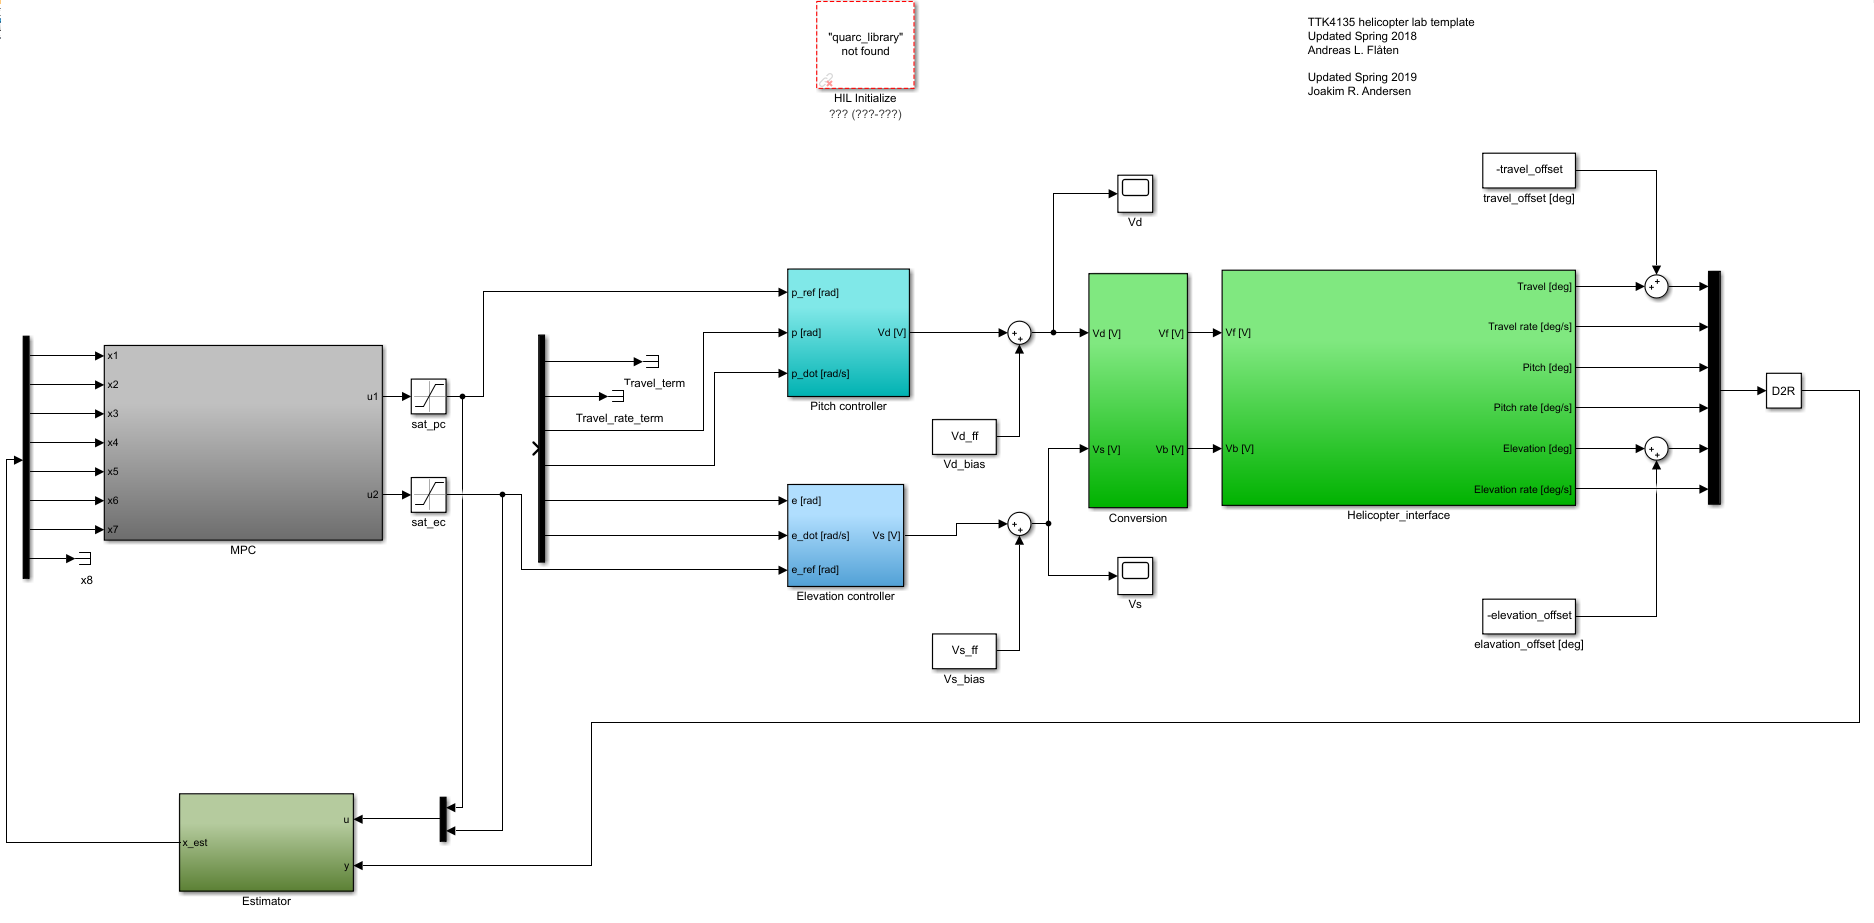
\includegraphics[angle=90,origin=c, scale=0.4]{fig/simulink/system.png}
    \caption{Simulink model}
    \label{fig:simulink_system}
\end{figure}

\begin{figure}
    \centering
    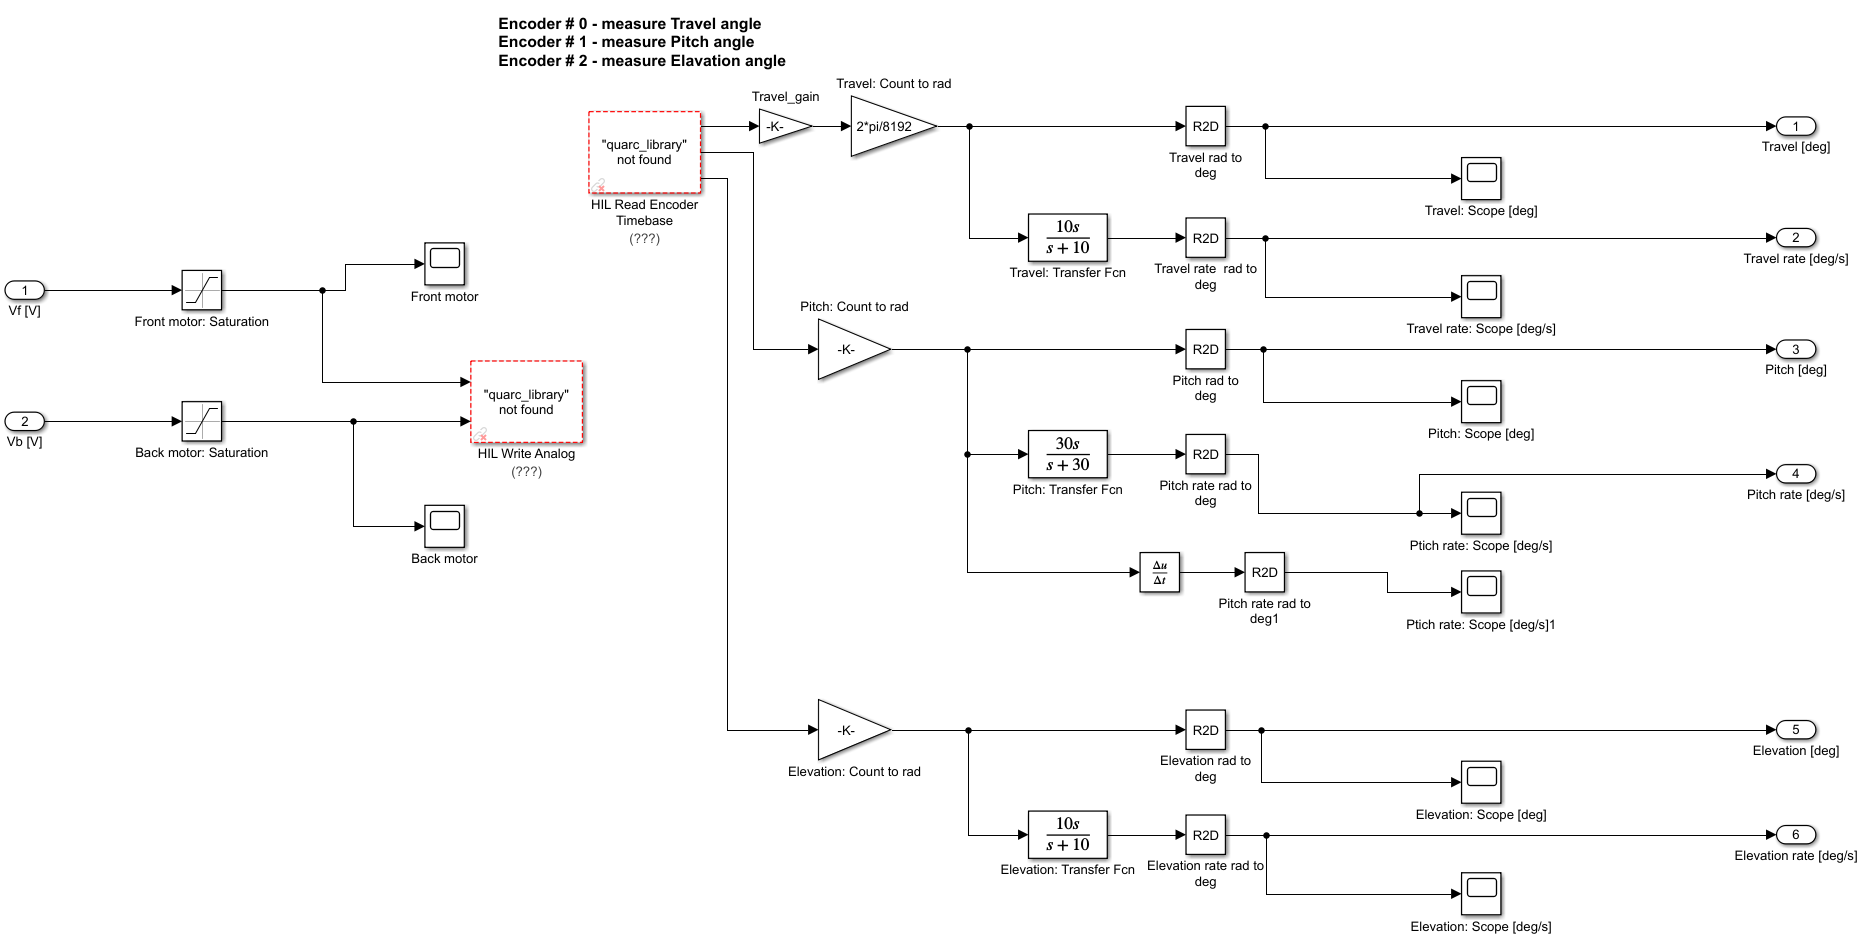
\includegraphics[scale=0.20]{fig/simulink/heli_interface.png}
    \caption{Helicopter interface}
    \label{fig:simulink_heli_interface}
\end{figure}

\begin{figure}
    \centering
    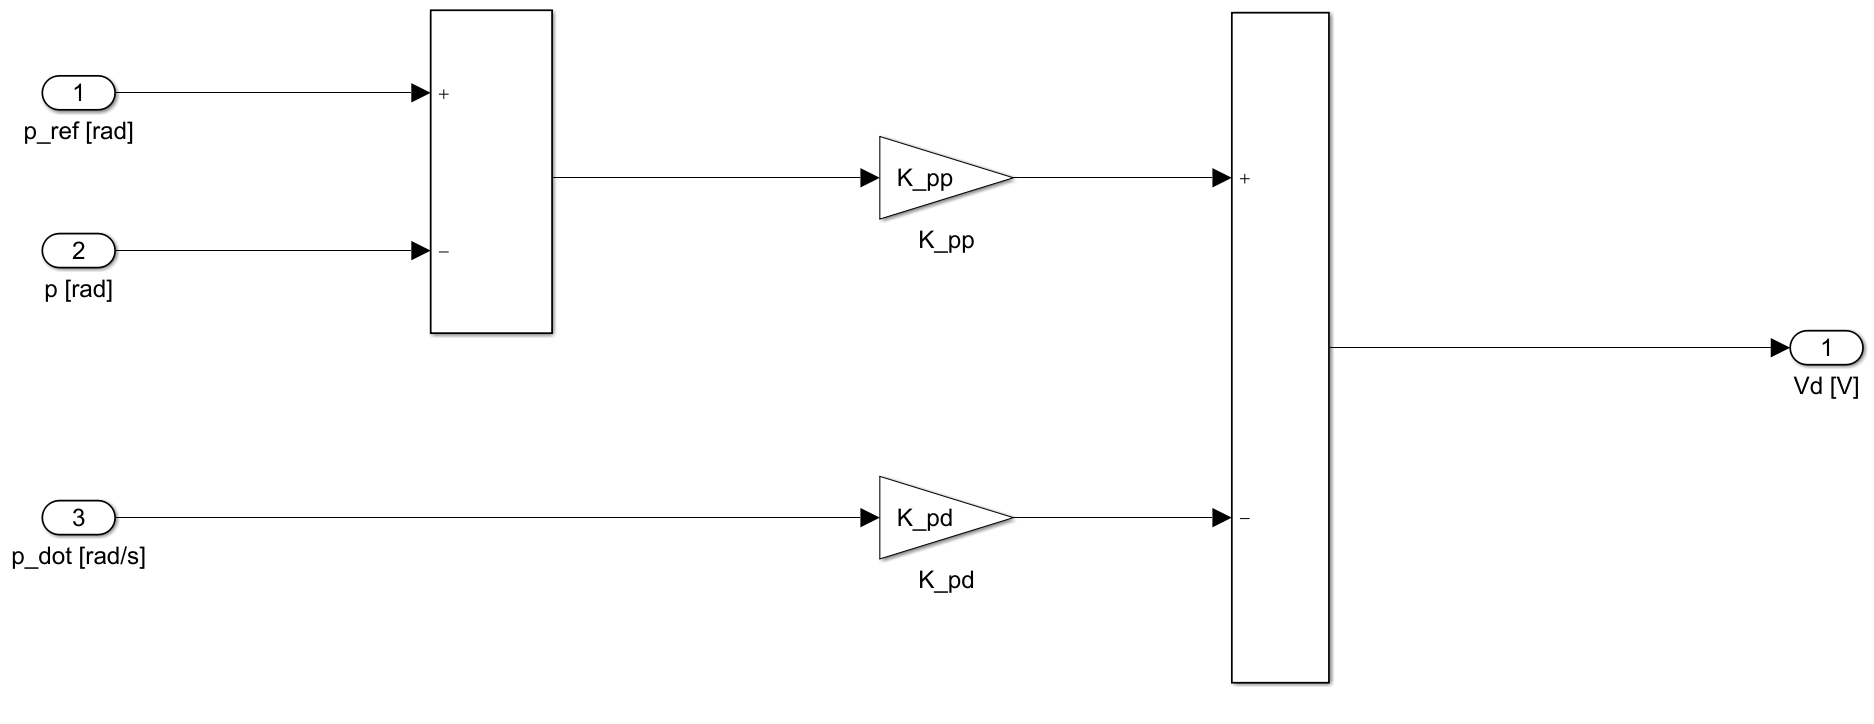
\includegraphics[scale=0.2]{fig/simulink/pitch_controller.png}
    \caption{Pitch controller}
    \label{fig:simulink_pitch_contr}
\end{figure}

\begin{figure}
    \centering
    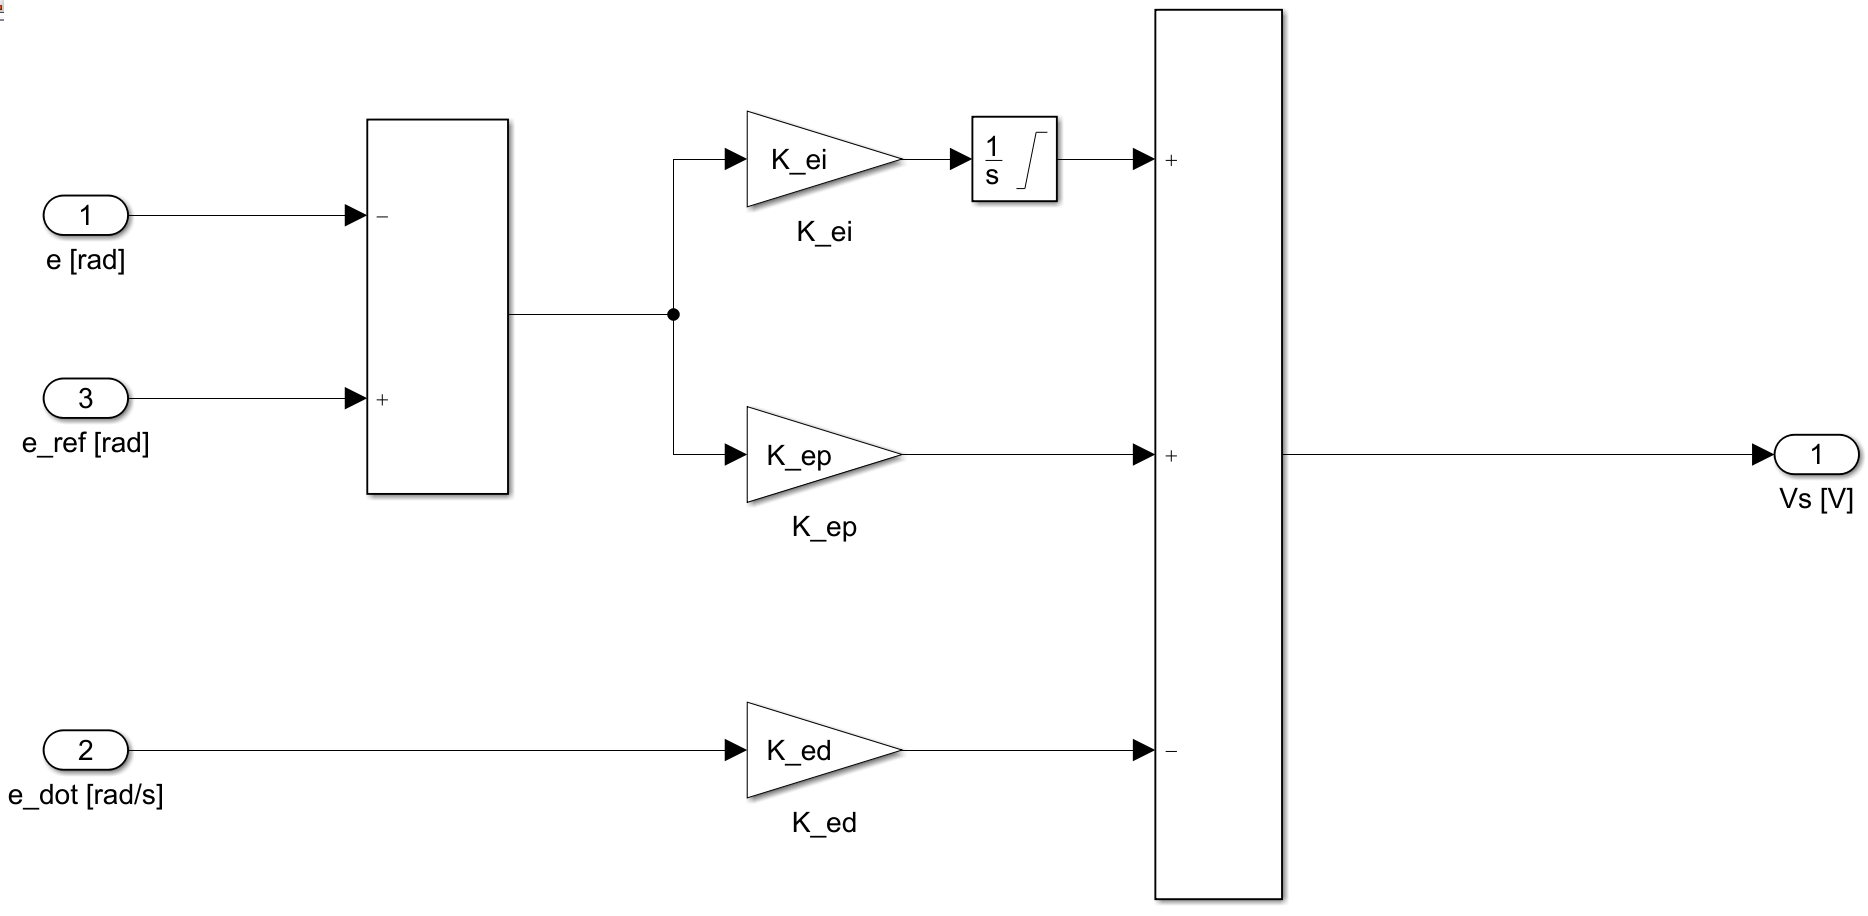
\includegraphics[scale=0.2]{fig/simulink/elevation_controller.png}
    \caption{Elevation controller}
    \label{fig:simulink_elev_contr}
\end{figure}

\begin{figure}
    \centering
    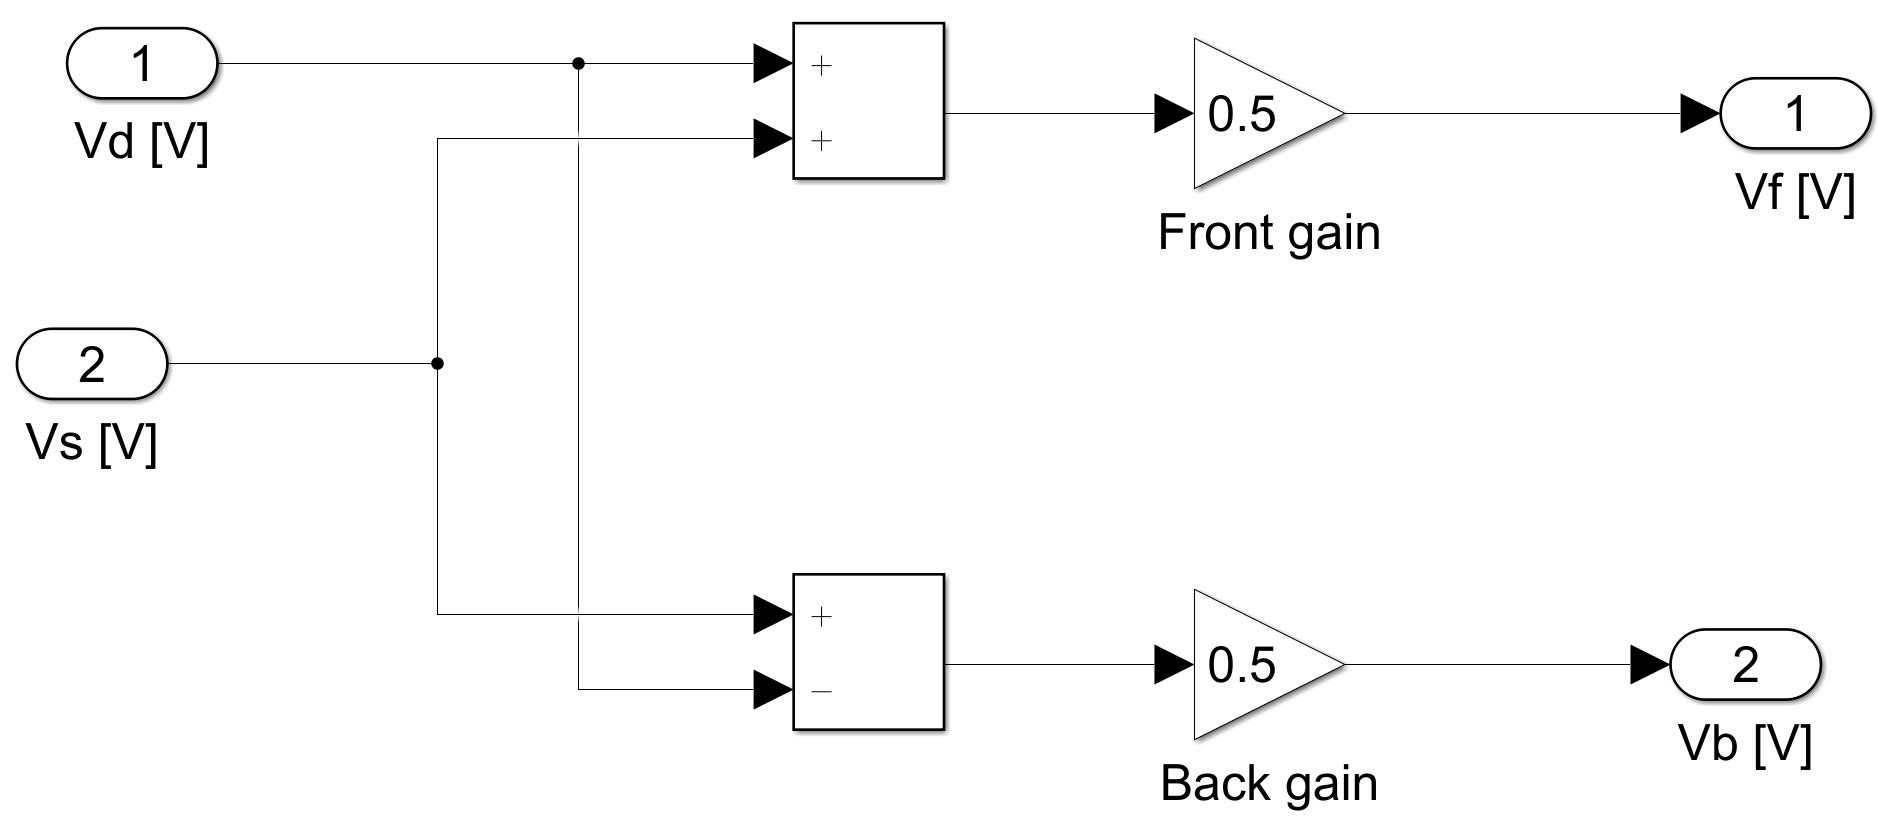
\includegraphics[scale=0.2]{fig/simulink/Vd_Vs_block.png}
    \caption{Voltage conversion block}
    \label{fig:simulink_Vd_Vs_block}
\end{figure}

\begin{figure}
    \centering
    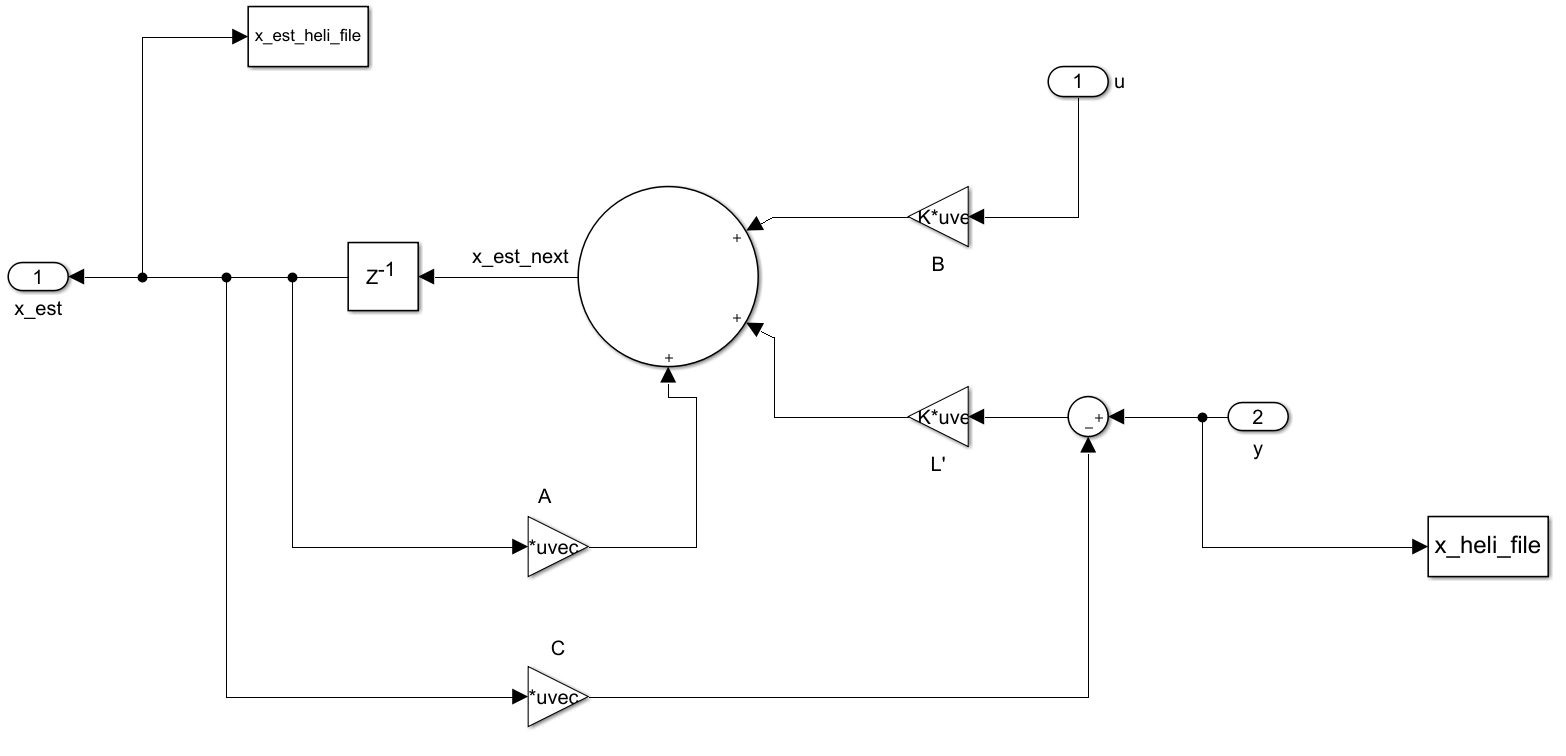
\includegraphics[scale=0.2]{fig/simulink/estimator.png}
    \caption{Estimator}
    \label{fig:simulink_estimator}
\end{figure}
\end{appendices}

\end{document}